\documentclass[12pt,oneside]{book}

% Extra functionality for command parsing, colouring elements, and commentary
\usepackage{xparse}
\usepackage[table,dvipsnames]{xcolor}
\usepackage{comment}

% Make \today only show month and year
\usepackage[en-CA]{datetime2}
\DTMlangsetup[en-CA]{showdayofmonth=false}

% Manifest data
%------------------------------------------------------------------------------
% Your Information
%------------------------------------------------------------------------------

\newcommand{\thesisType}{Thesis}

\newcommand{\thesisTitle}{My Thesis Title}
\newcommand{\thesisHalfTitle}{\thesisTitle}

\newcommand{\thesisAuthorName}{Johnny Appleseed}
\newcommand{\thesisAuthorNameShort}{J.\ Appleseed}
\newcommand{\thesisAuthorCredentials}{B.Sc.}
\newcommand{\thesisSupervisor}{Dr.\ Supervisor}

\newcommand{\thesisTargetDegreeNameShort}{M.Sc.}
\newcommand{\thesisTargetDegreeName}{Master of Science}

\newcommand{\thesisTargetDegreeFocus}{Computer Science}
\newcommand{\thesisTargetDegree}{\thesisTargetDegreeName{} in \thesisTargetDegreeFocus{}}

\newcommand{\thesisInstitutionDepartmentShort}{Computing and Software}
\newcommand{\thesisInstitutionGraduateStudies}{School of Graduate Studies}
\newcommand{\thesisInstitutionDepartment}{Department of \thesisInstitutionDepartmentShort{}}
\newcommand{\thesisInstitution}{McMaster University}
\newcommand{\thesisCityProvince}{Hamilton, Ontario}

\newcommand{\thesisSubmissionYear}{\the\year{}}
\newcommand{\thesisSubmissionMonthYear}{\DTMtoday{}}

%------------------------------------------------------------------------------
% Metadata
%------------------------------------------------------------------------------

% The label placed on the last page of the front matter is used to find how many
% pages belong in the front matter (which are numbered with roman numerals
% instead of the traditional arabic numbering system). You only need to update
% this label value IF the "Declaration of Academic Achievement" is not the last
% page of your front matter.
\newcommand{\thesisLastPageOfFrontMatterLabel}{chap:declaration_of_academic_achievement}

%------------------------------------------------------------------------------
% Options
%------------------------------------------------------------------------------

% - COMPILE FOR PRINTING THE PDF                              (default = false)
%   If enabled, 'porthref'* links will appear in footnotes to assist readers.
\newif\ifcompilingforprinting
% \compilingforprintingtrue % Enable
\compilingforprintingfalse % Disable

% - DOUBLE SPACING                                            (default = 2x)
% \newcommand{\thesisSpacing}{\doublespacing}
% \newcommand{\thesisSpacing}{\singlespacing}
\newcommand{\thesisSpacing}{\linespread{1}}

% - QUESTION-DIRECTED WRITING & TO-DOS SWITCH                 (default = true)
%   If enabled, "writing directive" boxes will be displayed in the PDF
\newif\ifshowwritingdirectives
\showwritingdirectivestrue % Show questions and to-do notes
% \showwritingdirectivesfalse % Don't show questions and to-do notes

% - RESET FOOTNOTE NUMBERING FOR EACH PAGE                    (default = false)
%   If enabled, the footnote numbering will reset to 1 on each new page
\newif\ifresetfootnotecounter
% \resetfootnotecountertrue % Reset footnote numbering on each page
\resetfootnotecounterfalse % Don't reset footnote numbering on each page

% - MARGIN SIZES
\newcommand{\thesisMarginTop}{3.8cm}                        % ("official" = 3.8cm)
\newcommand{\thesisMarginBottom}{2.5cm}                     % ("official" = 2.5cm)
\newcommand{\thesisMarginInner}{3.8cm}                      % ("official" = 3.8cm, recommended = 2.5cm)
\newcommand{\thesisMarginOuter}{2.5cm}                      % ("official" = 2.5cm)
\newcommand{\thesisMarginHeadheight}{15pt}                  % (default = 15pt)
\newcommand{\thesisTODOMarginSize}{3.5cm}                   % (default = 3.5cm, recommended = 2.25cm)


% Configure font and file encodings, and language as Canadian English
\usepackage{fontspec}
\setmainfont{Latin Modern Roman}
\usepackage[canadian]{babel}
\usepackage{lmodern}
\usepackage{anyfontsize}

% Math-related, but also generally helpful
\usepackage{proof}
\usepackage{amsmath}
\usepackage{amsfonts}
\usepackage{amsthm}
\usepackage{amssymb}
\usepackage{mathrsfs}
\usepackage{graphicx}
\usepackage{longtable}
\usepackage{svg}
\usepackage{mathpartir}
\usepackage{braket}

\usepackage{makecell, tabularx}
\renewcommand\theadalign{cc}
\renewcommand\theadfont{\bfseries}
\renewcommand\tabularxcolumn[1]{m{#1}}
\renewcommand{\arraystretch}{1.2}
\usepackage{pdflscape}
\usepackage{tablefootnote}

% Since LaTeX doesn't, and many fonts rarely, fully support unicode, we need to
% manually create characters to replace missing glyphs.
\usepackage{newunicodechar}
% At times, if you use raw unicode characters, you'll come across the following error:
% Missing character: There is no • (U+2022) in font ec-lmtt12!

% More, generally,
% Missing character: There is no `X` (U+`Y`) in font `Z`!

% To solve this  issue, we may manually replace instances of them with re-built
% copies of them. They may look a bit out of place because they don't follow the
% same font, but you can make them look decent if you replace them with simpler
% variants within the font. Try your best!

% For example, to resolve the above issue, we may use:
% \newunicodechar{•}{\(\cdot{}\)}

\newunicodechar{•}{\(\cdot{}\)}
\newunicodechar{‘}{\textquoteleft{}}
\newunicodechar{’}{\textquoteright{}}
\newunicodechar{≠}{\(\neq\)}


% Tiny package for easily grabbing the page count of the "main matter"
\usepackage{lastpage}

% For quotes, I wanted to put the "left bar" style. For implementation, Gonzalo
% Medina was very kind to create an example. It is based on:
% https://tex.stackexchange.com/a/50623
\usepackage{framed}
\usepackage[framemethod=TikZ]{mdframed}
\newmdenv[topline=false, rightline=false, bottomline=false,%
  linewidth=2pt, innerrightmargin=0pt, leftmargin=0pt,%
  innerleftmargin=5pt, skipabove=8pt, skipbelow=8pt]{mdleftbar}

\newmdenv[linewidth=2pt, linecolor=green, backgroundcolor=green!8, roundcorner=10pt,
  skipabove=8pt, skipbelow=8pt]{mdwritingdirectives}

% For nice captions and floating environments, such as for my code snippets
\usepackage{caption}
\usepackage{float}

% For inline-able list environments
\usepackage{paralist}

% Extra features for changing page widths ("adjustwidth" is a helpful environment!)
\usepackage{changepage}

% For code highlighting
\usepackage[newfloat,outputdir=build]{minted}
% Credits to Arash Esbati (https://tex.stackexchange.com/a/254177) for the
% listings-related component of minted usage.

\usemintedstyle{colorful}

% Configure page shape
\usepackage[
  a4paper,
  top=\thesisMarginTop{},
  bottom=\thesisMarginBottom{},
  inner=\thesisMarginInner{},
  outer=\thesisMarginOuter{},
  headheight=\thesisMarginHeadheight{},
]{geometry}

\usepackage{afterpage}

% Allow labelling enum items: Credits to: https://texblog.org/2012/03/21/cross-referencing-list-items/
\usepackage{enumitem}
\makeatletter
\def\namedlabel#1#2{\begingroup
    \textbf{#2}%
    \def\@currentlabel{#2}%
    \phantomsection\label{#1}\endgroup
}
\makeatother

\ifresetfootnotecounter
  % Make footnote counter reset for each new page.
  \usepackage{footnpag}
\fi

% Set spacing according to manifest
\usepackage{setspace}
\thesisSpacing{}

% Required for biblatex, but also adds functionality for quotation
\usepackage{csquotes}

% Jason's bibliography format
% % Credit to Gabriel Devenyi for this bibliography cfg:
% % github.com/gdevenyi/mcmaster.latex
% \usepackage[
%   style=numeric-comp,
%   backend=biber,
%   sorting=none,
%   backref=true,
%   maxnames=99,
%   alldates=iso,
%   seconds=true
% ]{biblatex} % bibliography
% \addbibresource{references.bib}
\usepackage[round]{natbib}
\bibliographystyle{plainnat}
\defcitealias{ISTQB}{Hamburg and Mogyorodi, 2024}

% Fancy Headers
\usepackage{fancyhdr}

% Allow more line breaks in URLs
\usepackage{xurl}

% Enable links within the document
\usepackage{hyperref}
\hypersetup{
  colorlinks=true,
  linkcolor=red,
  urlcolor=red,
  breaklinks=true,
  pdftitle={\thesisTitle{}},
  pdfauthor={\thesisAuthorName{}}
}
\urlstyle{rm} % Make URL styled fonts match hyperref's hrefs
\usepackage[nameinlink]{cleveref} % Fixes capitalization of internal references

\usepackage{nameref}

% For abbreviations, we use "acro" package, and mfirstuc to help capitalize long
% versions normally
\usepackage{array}
\usepackage{mfirstuc}
\MFUhyphentrue % tell mfirstuc to capitalize hyphenated words

% Acronyms
\usepackage{acro}
% For one-offs,
% \DeclareAcronym{acronym}{short=short-version,long=long-version}

\newcommand{\newacr}[2]{\DeclareAcronym{#1}{short=\uppercase{#1},long=#2}}
\newcommand{\newacrs}[3]{\DeclareAcronym{#1}{short=#2,long=#3}}

% Alphabetically sorted list of acronyms
\newacr{aop}{Aspect-Oriented Programming}
\newacr{api}{Application Programming Interface}
\newacr{ast}{Abstract Syntax Tree}
\newacr{cms}{Content Management System}
\newacr{cpu}{Central Processing Unit}
\newacr{csv}{Comma-Separated Values}
\newacr{dsl}{Domain-Specific Language}
\newacr{ffi}{Foreign Function Interface}
\newacr{gui}{Graphical User Interface}
\newacr{html}{HyperText Markup Language}
\newacr{href}{Hypertext REFerence}
\newacr{ide}{Integrated Development Environment}
\newacr{json}{JavaScript Object Notation}
\newacr{jvm}{Java Virtual Machine}
\newacr{mop}{MetaObject Protocol}
\newacr{nasa}{National Aeronautics and Space Administration}
\newacr{pdf}{Portable Document Format}
\newacr{sst}{Skeleton Syntax Tree}
\newacr{wysiwyg}{What You See Is What You Get}

% Case Studies 
%   (note: I'm grouping these together and forcing "newacrs" usage, even when
%    seemingly unneeded because, otherwise, they won't group together at the 
%    bottom of the complete "acronyms" list.)
\newacrs{glassbr}{GlassBR}{Glass Breaking}
\newacrs{projectile}{Projectile}{Projectile}
\newacrs{sglpend}{SglPend}{Single Pendulum}
\newacrs{dblpend}{DblPend}{Double Pendulum}
\newacrs{gamephysics}{GamePhysics}{Game Physics}
\newacrs{hghc}{HGHC}{Heat Transfer Coefficients between Fuel and Cladding in Fuel Rods}
\newacrs{pdcontroller}{PDController}{Proportional Derivative Controller}
\newacrs{swhs}{SWHS}{Solar Water Heating System}
\newacrs{nopcm}{SWHSNoPCM}{Solar Water Heating System Without PCM}
\newacrs{ssp}{SSP}{Slope Stability analysis Program}


%------------------------------------------------------------------------------
%- Extra commands for more functionality -- in particular, capitalizing the
%- long form of acronyms.
%------------------------------------------------------------------------------

% Defining \ACL - to capitalize all words in an acronym
% Credits to: https://tex.stackexchange.com/a/257896
\NewDocumentCommand\ACF{sm}{%
  \begingroup
  \acsetup{uppercase/cmd=\ecapitalisewords}%
  \IfBooleanTF{#1}{\Acf*{#2}}{\Acf{#2}}%
  \endgroup
}

\NewDocumentCommand\ACFP{sm}{%
  \begingroup
  \acsetup{uppercase/cmd=\ecapitalisewords}%
  \IfBooleanTF{#1}{\Acfp*{#2}}{\Acfp{#2}}%
  \endgroup
}

\NewDocumentCommand\ACL{sm}{%
  \begingroup
  \acsetup{uppercase/cmd=\ecapitalisewords}%
  \IfBooleanTF{#1}{\Acl*{#2}}{\Acl{#2}}%
  \endgroup
}

\NewDocumentCommand\ACLP{sm}{%
  \begingroup
  \acsetup{uppercase/cmd=\ecapitalisewords}%
  \IfBooleanTF{#1}{\Aclp*{#2}}{\Aclp{#2}}%
  \endgroup
}


% General Utility Functions
%------------------------------------------------------------------------------
% Question-directed Writing
%------------------------------------------------------------------------------

\ifshowwritingdirectives
  \newenvironment{writingdirectives}{\begin{mdwritingdirectives}\centering\textbf{Writing Directives}\begin{itemize}}{\end{itemize}\end{mdwritingdirectives}}
\else
  \excludecomment{writingdirectives}
\fi

%------------------------------------------------------------------------------
% Spacing Options
%------------------------------------------------------------------------------

\newcommand{\thesisForceSingleSpacing}{\singlespacing}
\newcommand{\thesisForceDoubleSpacing}{\doublespacing}

%------------------------------------------------------------------------------
% Footnotes that only show when "compiling for printing."
%------------------------------------------------------------------------------

\ifcompilingforprinting
  \newcommand{\printOnlyFootnote}[1]{\footnote{#1}}
  \newcommand{\printOnlyFootnoteText}[1]{\footnotetext{#1}}
  \newcommand{\printOnlyFootnoteMark}{\footnotemark}
\else
  \newcommand{\printOnlyFootnote}[1]{}
  \newcommand{\printOnlyFootnoteText}[1]{}
  \newcommand{\printOnlyFootnoteMark}{}
\fi

%------------------------------------------------------------------------------
% Portable HREFs
%------------------------------------------------------------------------------

% Common variant
\newcommand{\porthref}[2]{\href{#2}{#1}\printOnlyFootnote{\url{#2}}}

% Custom URLs
\newcommand{\porthreft}[3]{\href{#3}{#1}\printOnlyFootnote{\href{#3}{#2}}}
% Inside of some environments, footnote marks aren't registered properly, so we
% need to manually write the "text" part
\newcommand{\porthreftm}[2]{\href{#2}{#1\printOnlyFootnoteMark}}

%------------------------------------------------------------------------------
% TODOs
%------------------------------------------------------------------------------

% Generic Inlined TODOs
\newcommand{\intodo}[1]{\todo[inline]{#1}}

% Unimportant TODOs for "later" (i.e., finishing touches or changes immediately before submission)
\newcommand{\latertodo}[1]{\todo[backgroundcolor=Cyan]{\textit{Later}: #1}}

% "Important" TODOs
\newcommand{\imptodo}[1]{\todo[inline,backgroundcolor=Red]{\textbf{Important}: #1}}

% "Easy" TODOs
\newcommand{\easytodo}[1]{\todo[inline,backgroundcolor=SeaGreen]{\textit{Easy}: #1}}
\newcommand{\eztodo}[1]{\easytodo{#1}}

% "Tedious" TODOs
\newcommand{\tedioustodo}[1]{\todo[inline,backgroundcolor=PineGreen]{\textit{Needs time}: #1}}

% "Question" TODO Notes
\newcounter{todonoteQuestionsCtr}
\newcommand{\questiontodo}[1]{\stepcounter{todonoteQuestionsCtr}\todo[backgroundcolor=Lavender]{\textbf{Q \#\thetodonoteQuestionsCtr{}}: #1}}
\newcommand{\qtodo}[1]{\questiontodo{#1}}

%------------------------------------------------------------------------------
% Code Snippets
%------------------------------------------------------------------------------

\newenvironment{code}{\captionsetup{type=listing,skip=14pt}}{}
\SetupFloatingEnvironment{listing}{name=Source Code, listname=List of Source Codes}
\crefname{listing}{source code}{source codes}
\Crefname{listing}{Source Code}{Source Codes}

\newenvironment{haskell}[3]
{\VerbatimEnvironment\thesisForceSingleSpacing{}\begin{code}\captionof{listing}[#1]{\protect\porthreftm{#1}{#3}}\printOnlyFootnoteText{\protect\url{#3}}\label{lst:#2}\begin{minted}[frame=lines,framerule=2pt,breaklines]{haskell}}
  {\end{minted}\end{code}\thesisSpacing{}}

\newenvironment{codeSnippet}[4]
{\VerbatimEnvironment\thesisForceSingleSpacing{}\begin{code}\captionof{listing}[#2]{\protect\porthreftm{#2}{#4}}\printOnlyFootnoteText{\protect\url{#4}}\label{lst:#3}\begin{minted}[frame=lines,framerule=2pt,breaklines]{#1}}
  {\end{minted}\end{code}\thesisSpacing{}}

\newenvironment{pseudohaskell}[2]
{\VerbatimEnvironment\thesisForceSingleSpacing{}\begin{code}\captionof{listing}{Pseudocode: #1}\label{lst:#2}\begin{minted}[frame=lines,framerule=2pt,breaklines]{haskell}}
  {\end{minted}\end{code}\thesisSpacing{}}

\newenvironment{pseudocode}[3]
{\VerbatimEnvironment\thesisForceSingleSpacing{}\begin{code}\captionof{listing}{Pseudocode: #2}\label{lst:#3}\begin{minted}[frame=lines,framerule=2pt,breaklines]{#1}}
  {\end{minted}\end{code}\thesisSpacing{}}

\newcommand{\inlineHs}[1]{\mintinline{haskell}|#1|}
\newcommand{\inlineCode}[2]{\mintinline{#1}|#2|}

%------------------------------------------------------------------------------
% Link to Drasil issue
%------------------------------------------------------------------------------

\newcommand{\issueref}[1]{\href{https://github.com/JacquesCarette/Drasil/issues/#1}{\##1}}
\newcommand{\pullref}[1]{\href{https://github.com/JacquesCarette/Drasil/pull/#1}{\##1}}
\newcommand{\thesisissueref}[1]{\href{https://github.com/samm82/TestGen-Thesis/issues/#1}{\##1}}



% General Assets
%------------------------------------------------------------------------------
% Code
%------------------------------------------------------------------------------

% Command based on: https://tex.stackexchange.com/questions/266811/define-a-new-command-with-parameters-inside-newcommand
\newcommand{\codeName}[1]{\expandafter\newcommand\csname #1\endcsname{\inlineHs{#1}}}

% Used for showing what the blue-highlighted text is, in the reading notes section
\codeName{ExampleText}

% Defines commands to be used in poster and thesis

\newcommand{\swebokScalDef}{This seems to define ``usability
    testing'' with elements of functional and recovery testing}
\newcommand{\swebokElasRef}{only cites a single source
    \textbf{that doesn't contain the words ``elasticity'' or ``elastic''}!}

% for assets/code/example.tex...
\newcommand{\exampleCode}{\begin{codeSnippet}{haskell}{``MultiDefinitions'' (MultiDefn) Definition}{exampleCode}{https://github.com/JacquesCarette/Drasil/blob/051b9881a6417e51e818c6673c5eab0f48bd5af2/code/drasil-theory/lib/Theory/Drasil/MultiDefn.hs\#L45-L56}
-- | 'MultiDefn's are QDefinition factories, used for showing one or more ways
--   we can define a QDefinition.
data MultiDefn e = MultiDefn{
  -- | UID
  _rUid :: UID,
  -- | Underlying quantity it defines.
  _qd :: QuantityDict,
  -- | Explanation of the different ways we can define a quantity.
  _rDesc :: Sentence,
  -- | All possible ways we can define the related quantity.
  _rvs :: NE.NonEmpty (DefiningExpr e)
}
\end{codeSnippet}
}
\newcommand{\refExampleCode}{\Cref{lst:exampleCode}}

% for assets/code/examplePseudocode.tex...
\newcommand{\examplePseudocode}{\begin{pseudocode}{haskell}{Broken QuantityDict Chunk Retriever}{examplePseudocode}
retrieveQD :: UID -> ChunkDB -> Maybe QuantityDict
retrieveQD u cdb = do
    (Chunk expectedQd) <- lookup u cdb
    pure expectedQd
\end{pseudocode}
}
\newcommand{\refExamplePseudocode}{\Cref{lst:examplePseudocode}}

% for assets/code/mainInvalidInputTest.tex...
\newcommand{\mainInvalidInputTest}{\begin{codeSnippet}{python}{Tests for main with an invalid input file}{mainInvalidInputTest}{https://github.com/samm82/Drasil/blob/sysTests/code/stable/projectile/projectile_c_p_nol_b_u_v_d/src/python/test/Control_test.py\#L29-L53}
  # from https://stackoverflow.com/questions/54071312/how-to-pass-command-line-argument-from-pytest-to-code
  ## \brief Tests main with invalid input file
  # \par Types of Testing:
  # Dynamic Black-Box (Behavioural) Testing
  # Boundary Conditions
  # Default, Empty, Blank, Null, Zero, and None
  # Invalid, Wrong, Incorrect, and Garbage Data
  # Logic Flow Testing
  @mark.parametrize("filename", invalid_value_input_files)
  @mark.xfail
  def test_main_invalid(monkeypatch, filename):
      # from https://stackoverflow.com/questions/10840533/most-pythonic-way-to-delete-a-file-which-may-not-exist
      try:
          remove(output_filename)
      except OSError as e: # this would be "except OSError, e:" before Python 2.6
          if e.errno != ENOENT: # no such file or directory
              raise # re-raise exception if a different error occurred


      assert not path.exists(output_filename)


      with monkeypatch.context() as m:
          m.setattr(sys, 'argv', ['Control.py', str(Path("test/test_input") / f"{filename}.txt")])
          Control.main()
      
      assert not path.exists(output_filename)
\end{codeSnippet}
}
\newcommand{\refMainInvalidInputTest}{\Cref{lst:mainInvalidInputTest}}

% for assets/code/projManualViolationReq.tex...
\newcommand{\projManualViolationReq}{\begin{codeSnippet}{haskell}{\acs{projectile}'s manually created requirement for constraint violation behaviour}{projManualViolationReq}{https://github.com/JacquesCarette/Drasil/blob/afb6fb752b8364d2807ced7fc0c1dd6c6aba52b2/code/drasil-example/projectile/lib/Drasil/Projectile/Requirements.hs\#L31-L34}
verifyParamsDesc = foldlSent [S "Check the entered", plural inValue,
    S "to ensure that they do not exceed the" +:+. namedRef (datCon [] []) (plural datumConstraint),
    S "If any of the", plural inValue, S "are out of bounds" `sC`
    S "an", phrase errMsg, S "is displayed" `S.andThe` plural calculation, S "stop"]
\end{codeSnippet}
}
\newcommand{\refProjManualViolationReq}{\Cref{lst:projManualViolationReq}}

% for assets/code/projViolationChoice.tex...
\newcommand{\projViolationChoice}{\begin{codeSnippet}{haskell}{\acs{projectile}'s choice for constraint violation behaviour in code}{projViolationChoice}{https://github.com/JacquesCarette/Drasil/blob/afb6fb752b8364d2807ced7fc0c1dd6c6aba52b2/code/drasil-example/projectile/lib/Drasil/Projectile/Choices.hs\#L120}
    srsConstraints = makeConstraints Warning Warning,
\end{codeSnippet}
}
\newcommand{\refProjViolationChoice}{\Cref{lst:projViolationChoice}}

%------------------------------------------------------------------------------
% Graphs
%------------------------------------------------------------------------------

% Organization of files

\newcommand{\parChdGraphs}{
    % Only top or bottom to comply with IEEE guidelines
    \begin{figure}[bt!]
        \centering
        \begin{subfigure}[b]{\linewidth}
            \centering
            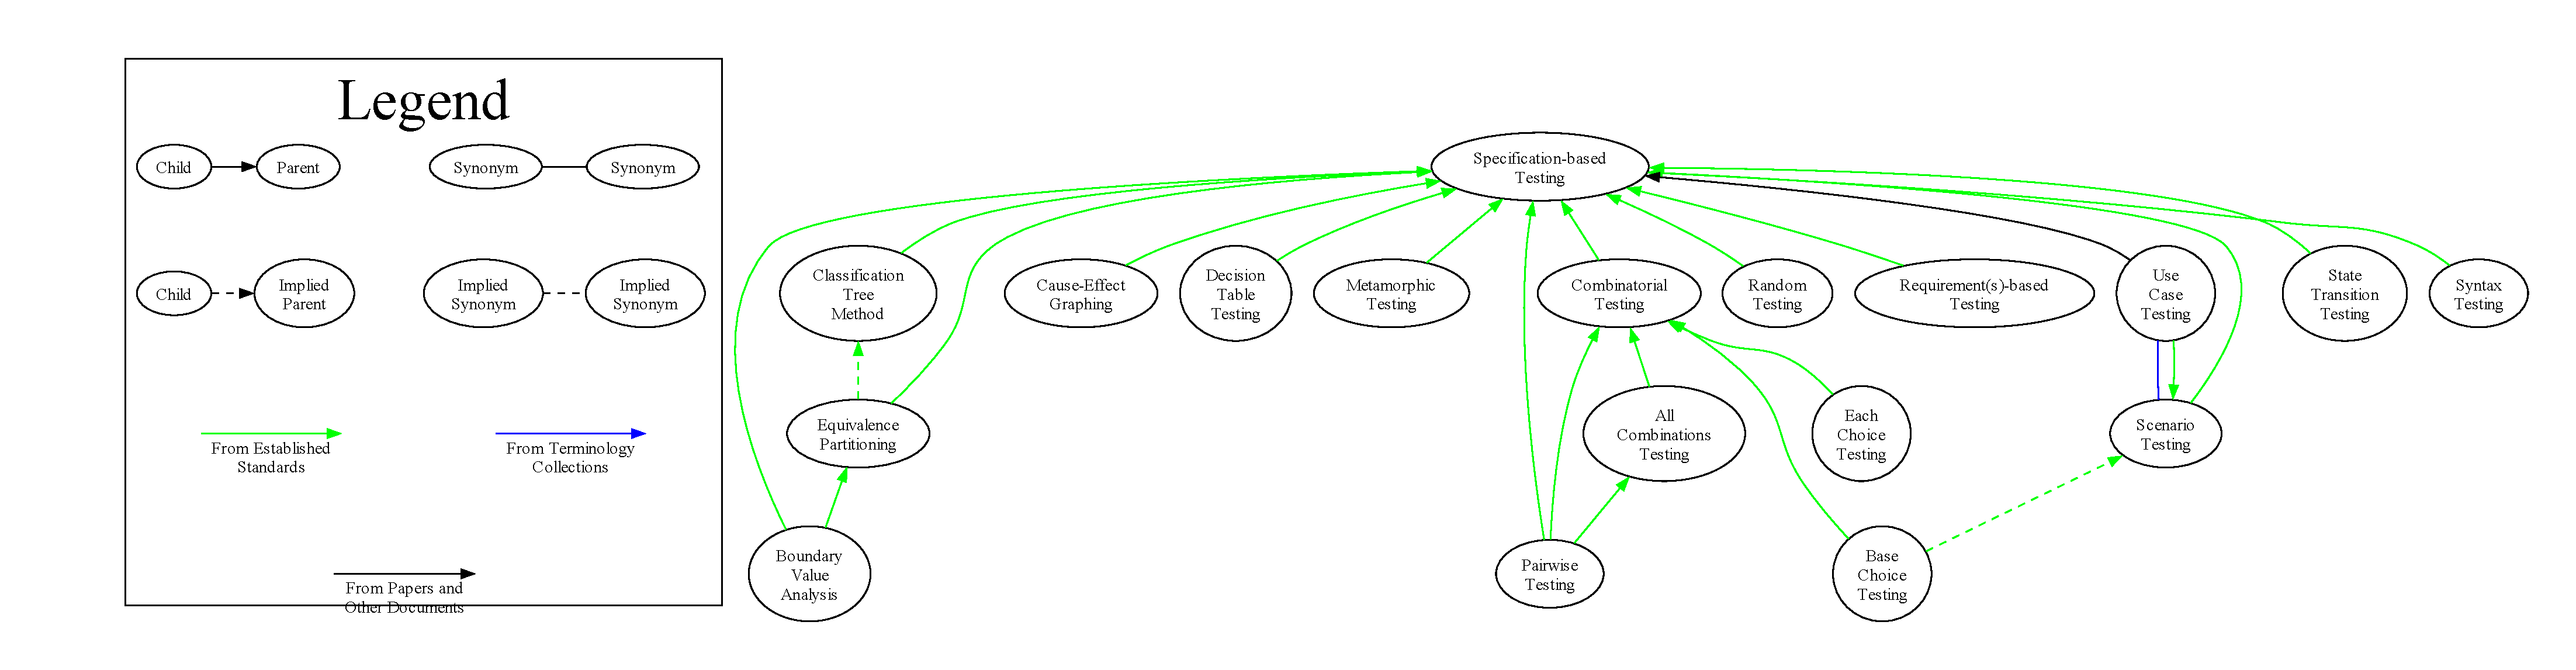
\includegraphics[width=\linewidth]{assets/graphs/specBasedGraph.pdf}
            \caption{``Superset'' relations.}
            \label{fig:specBasedGraph}
        \end{subfigure}
        \begin{subfigure}[t]{.45\linewidth}
            \centering
            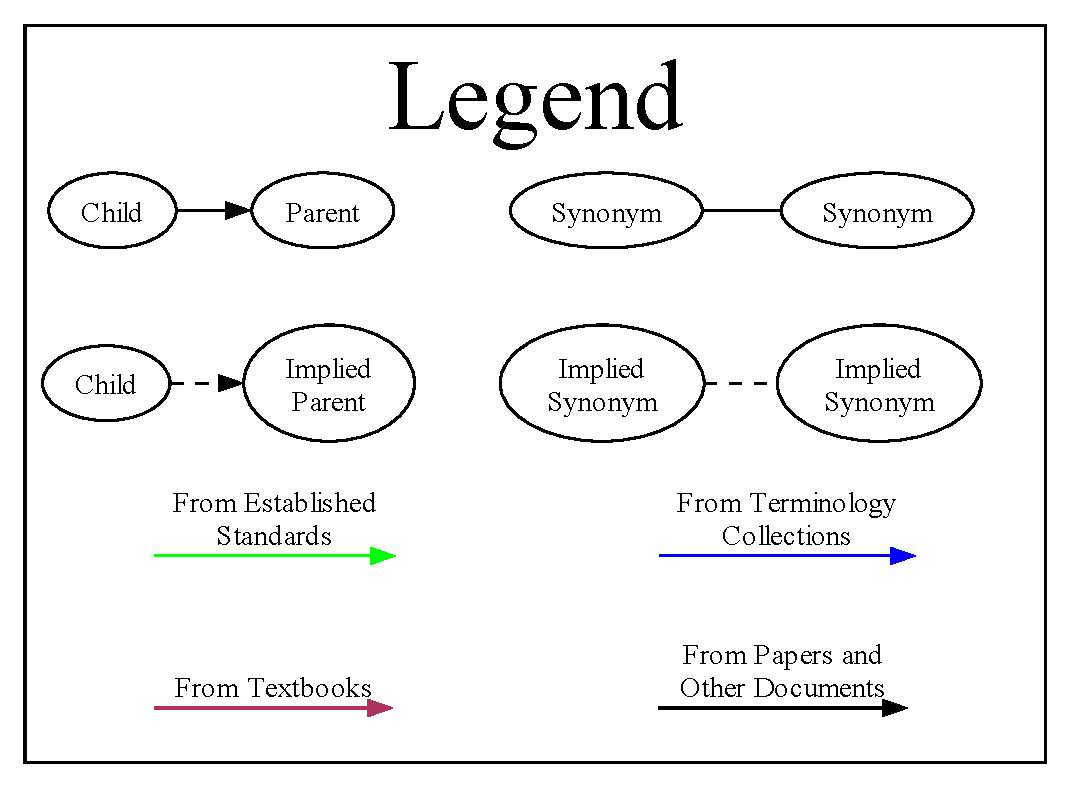
\includegraphics[width=\linewidth]{assets/graphs/parChdLegend.pdf}
        \end{subfigure}
        \begin{subfigure}[t]{.5\linewidth}
            \centering
            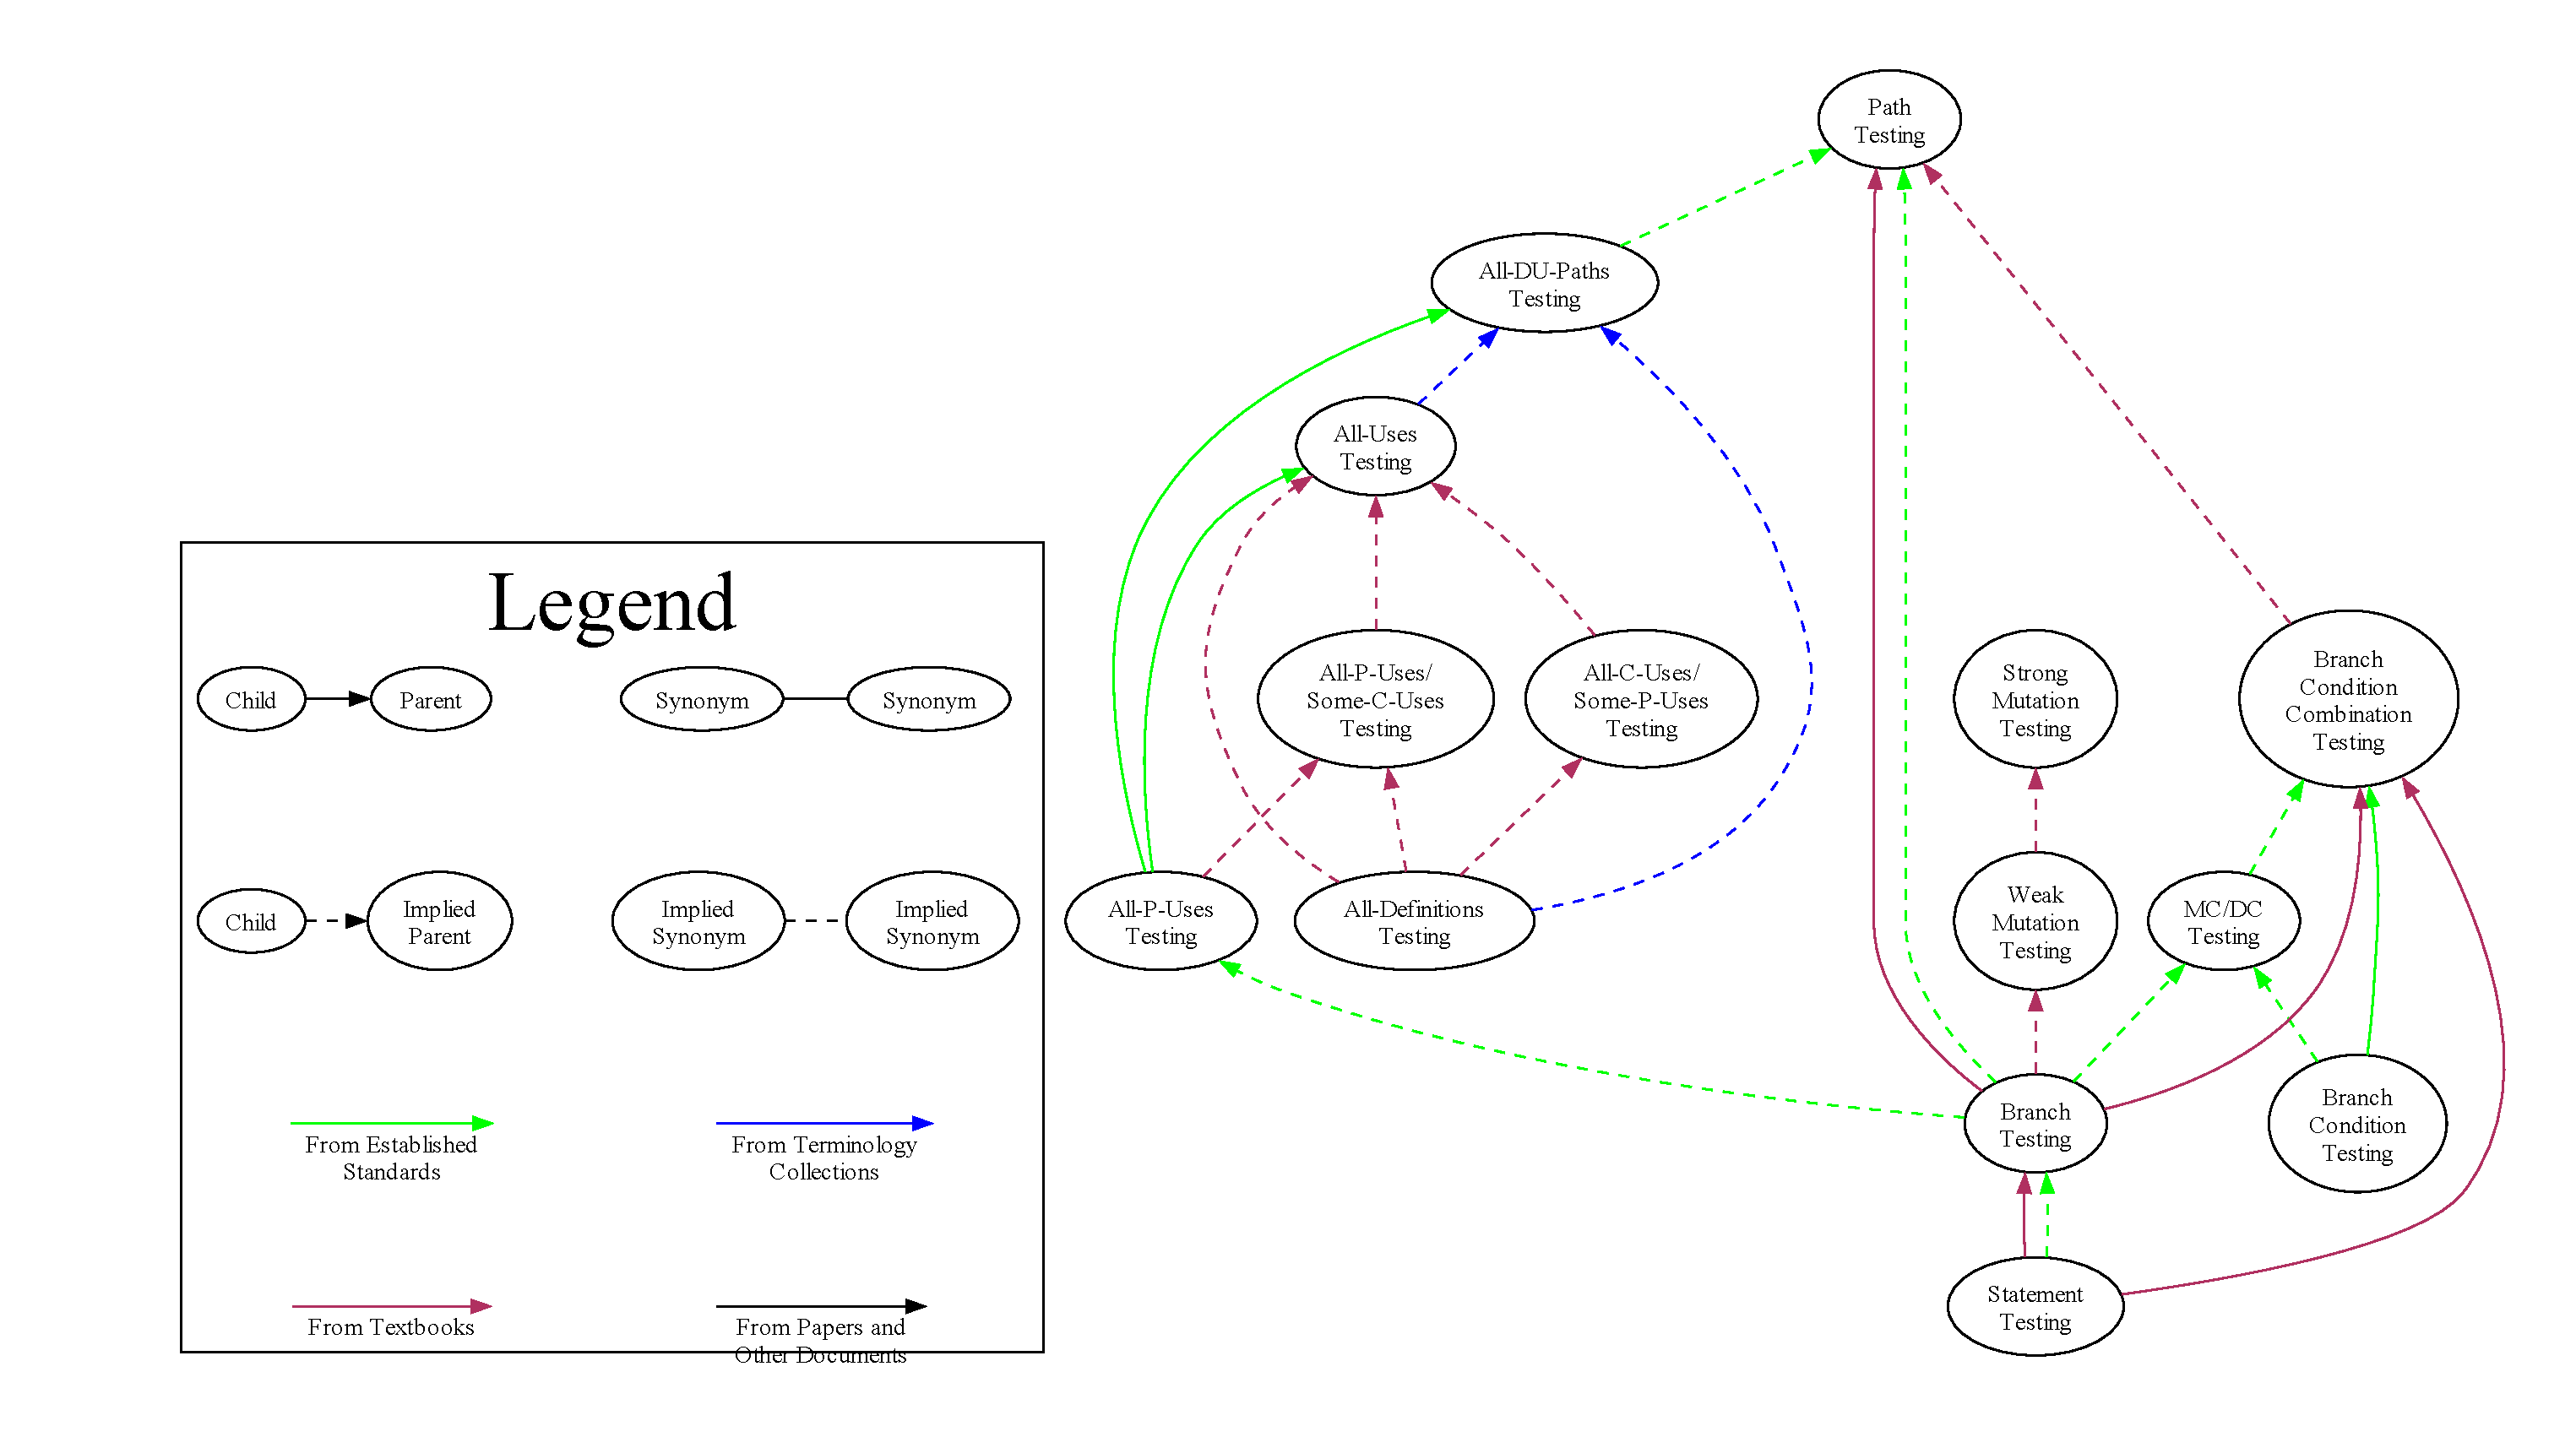
\includegraphics[width=\linewidth]{assets/graphs/subsumesGraph.pdf}
            \caption{``Subsume'' relations.}
            \label{fig:subsumesGraph}
        \end{subfigure}
        \caption{Graphs of different classes of \hyperref[par-chd-rels]{parent-child relations}.}
        \label{fig:parChdGraphs}
    \end{figure}
}

\newcommand{\ExampleGraph}{
    \begin{figure*}
        \begin{subfigure}[b]{0.3\linewidth}
            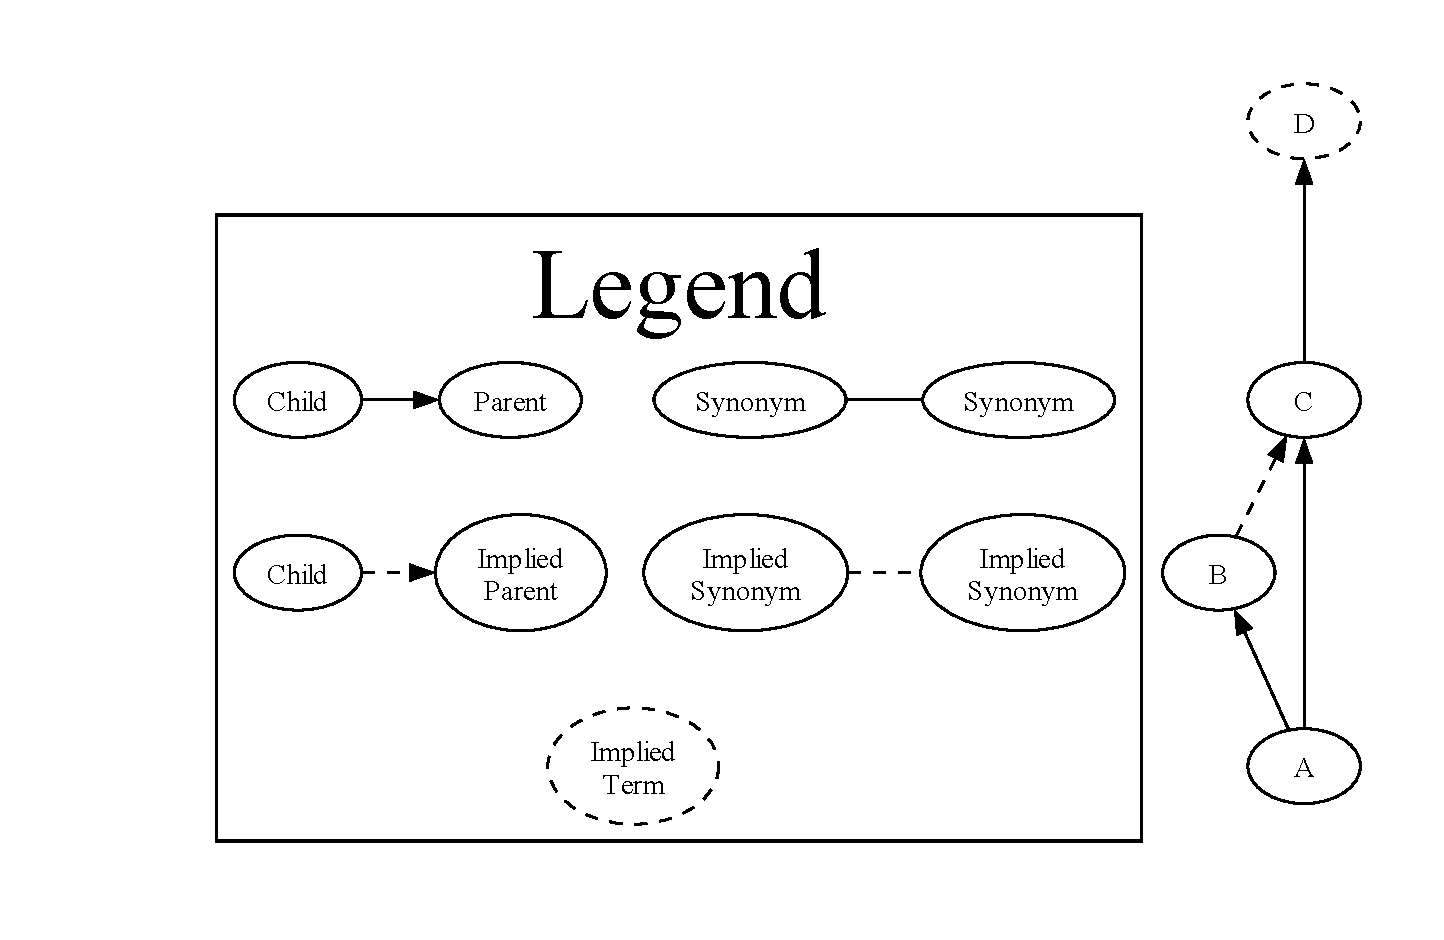
\includegraphics[width=\linewidth]{assets/graphs/ExampleGlossaryGraph.pdf}
            \caption{Graph from \Cref{tab:exampleGlossary}.}
            \label{fig:exampleGraph}
        \end{subfigure}
        \centering
        \begin{subfigure}[b]{0.675\linewidth}
            \centering
            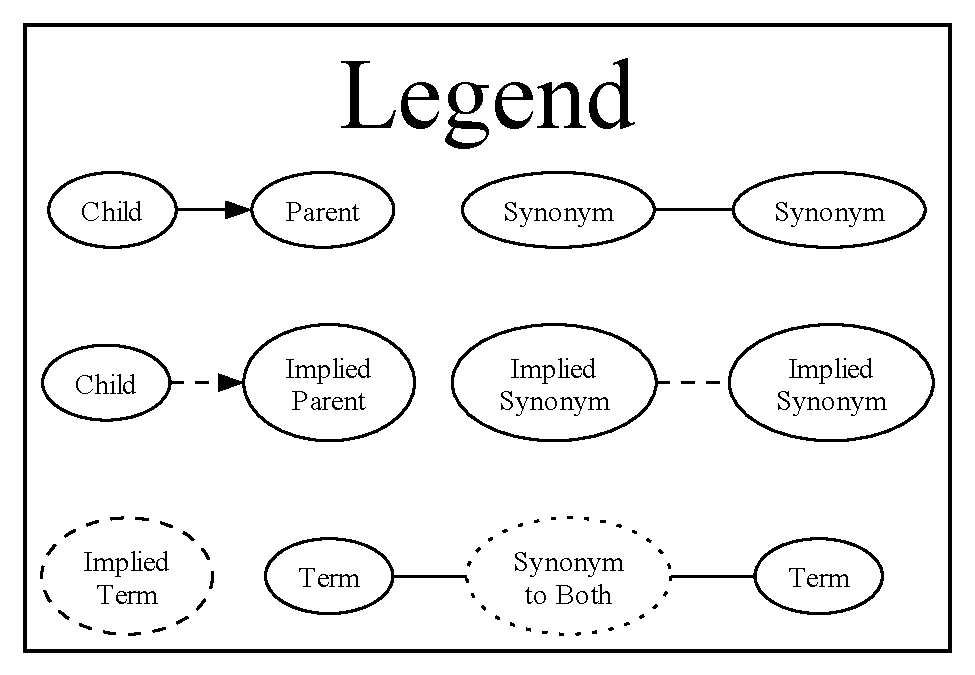
\includegraphics[width=0.8\linewidth]{assets/graphs/manual/manualLegendNonSolidTerms.pdf}
            \hspace{5cm}\begin{subfigure}[t]{0.475\linewidth}
                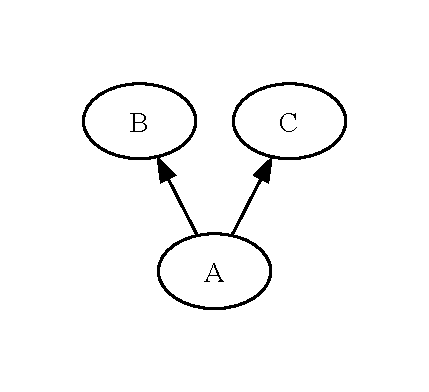
\includegraphics[width=1.1\linewidth]{assets/graphs/rigidExampleGlossaryGraph.pdf}
                \caption{Rigid graph from\\\Cref{tab:exampleGlossary}.}
                \label{fig:rigidExampleGraph}
            \end{subfigure}
            \begin{subfigure}[t]{0.475\linewidth}
                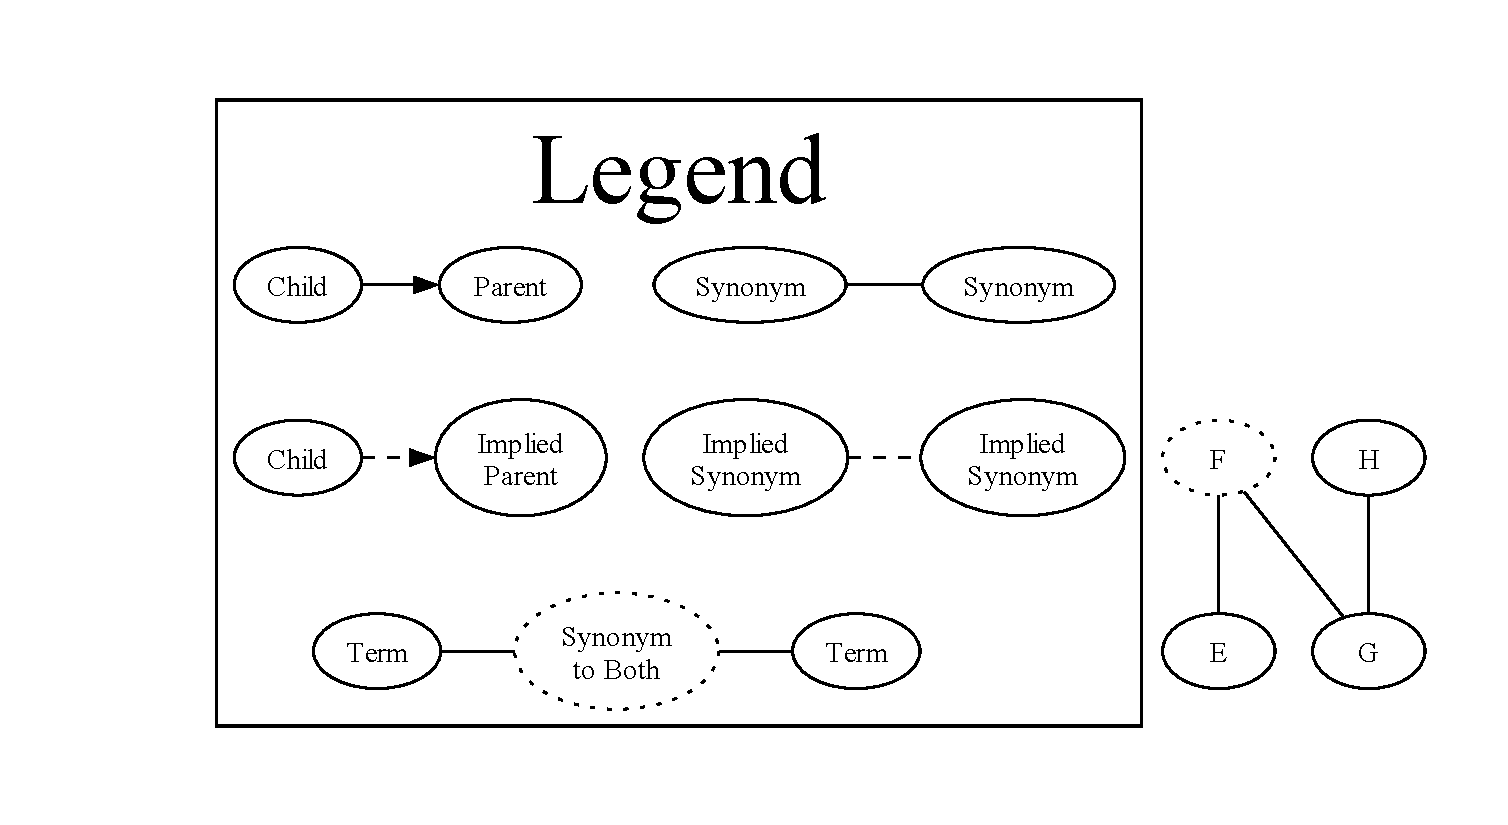
\includegraphics[width=1.1\linewidth]{assets/graphs/SynExampleGlossaryGraph.pdf}
                \caption{Graph from \Cref{tab:synExampleGlossary}.}
                \label{fig:synExampleGraph}
            \end{subfigure}
        \end{subfigure}
        \begin{subfigure}[t]{0.25\linewidth}
            \centering
            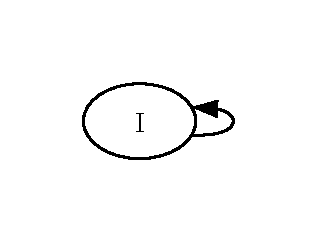
\includegraphics[width=1.2\linewidth]{assets/graphs/SelfExampleGlossaryGraph.pdf}
            \caption{Self-loop graph.}
            \label{fig:selfExampleGraph}
        \end{subfigure}
        \hfill
        \begin{subfigure}[t]{0.425\linewidth}
            \centering
            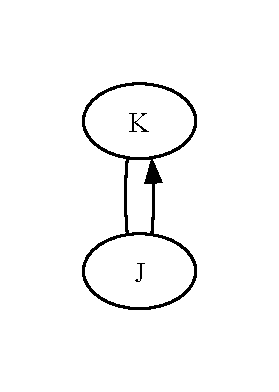
\includegraphics[width=0.6\linewidth]{assets/graphs/ParSynExampleGlossaryGraph.pdf}
            \caption{Graph of a pair of terms with a \hyperref[par-chd-rels]{parent-child} \emph{and} synonym relation.}
            \label{fig:parSynExampleGraph}
        \end{subfigure}
        \hfill
        \begin{subfigure}[t]{0.25\linewidth}
            \centering
            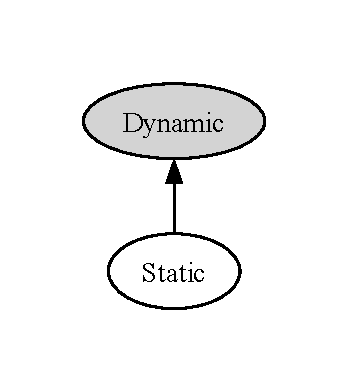
\includegraphics[width=1.4\linewidth]{assets/graphs/StaticExampleGlossaryGraph.pdf}
            \caption{Static graph.}
            \label{fig:staticExampleGraph}
        \end{subfigure}
        \caption{Example generated graphs.}
        \label{fig:exampleGraphs}
    \end{figure*}
}

\newcommand{\recoveryGraphs}{
    % Only top or bottom to comply with IEEE guidelines
    \begin{figure}[bt!]
        \centering
        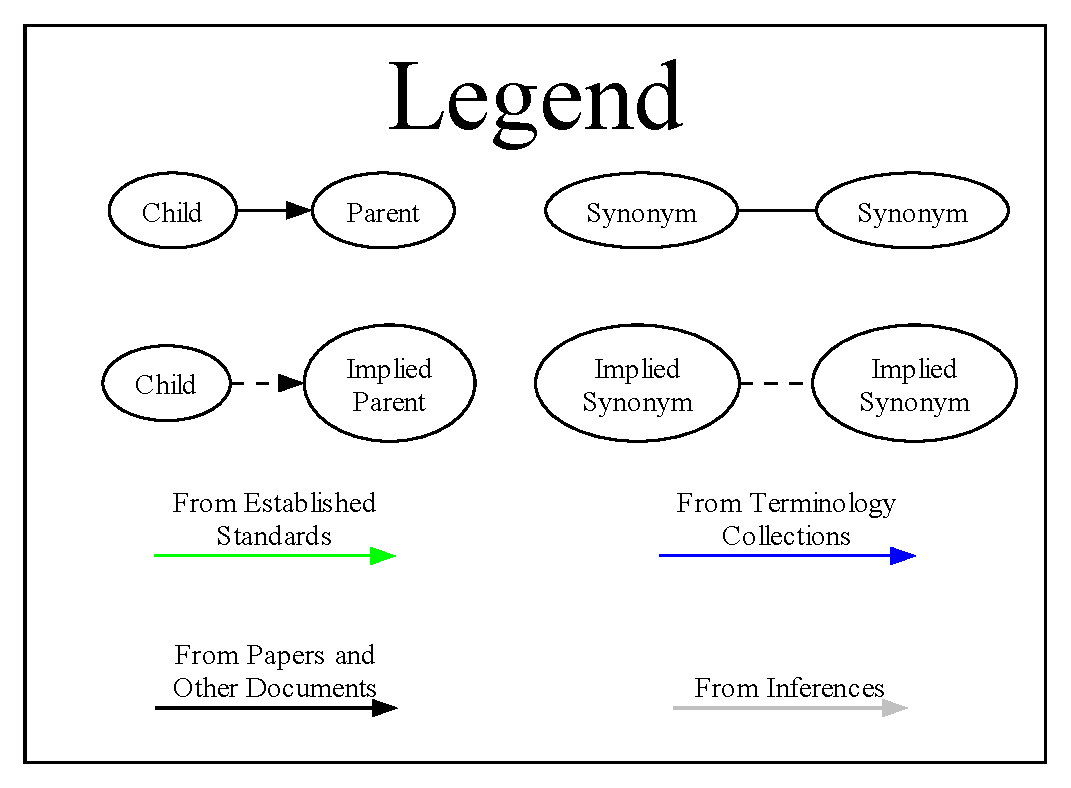
\includegraphics[width=\linewidth]{assets/graphs/recoveryLegend.pdf}
        \begin{subfigure}[b]{.55\linewidth}
            \centering
            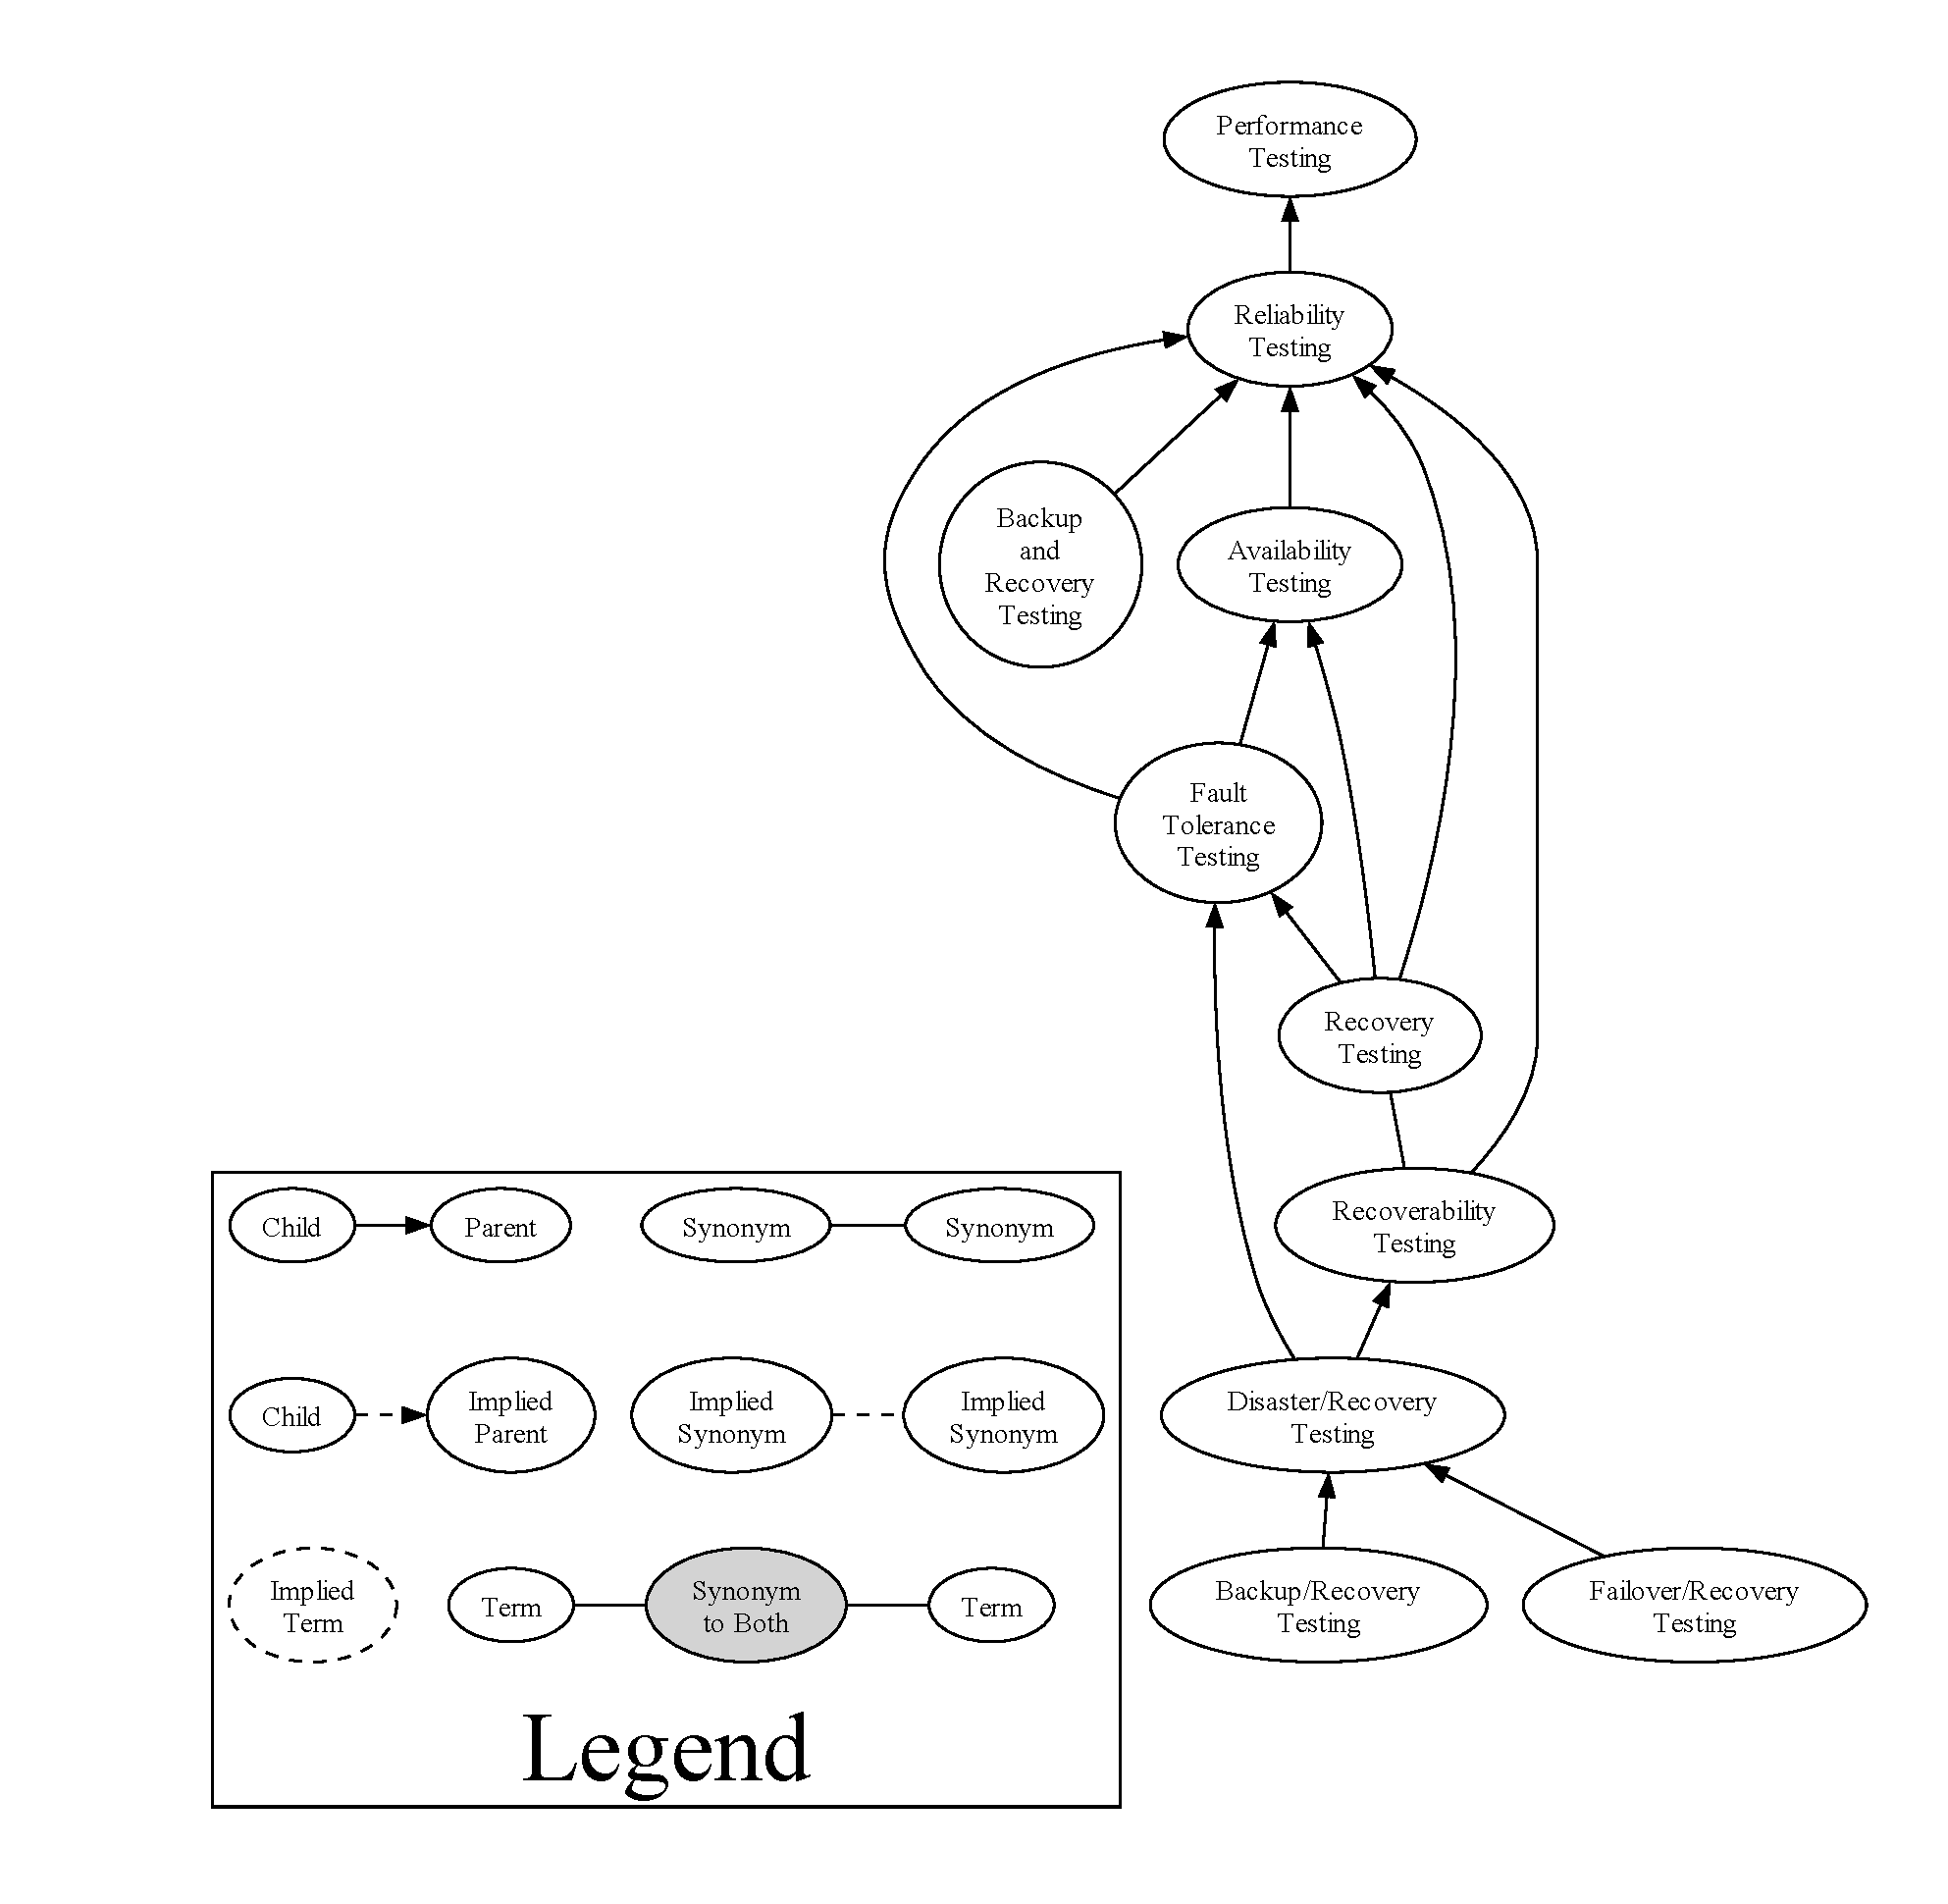
\includegraphics[width=\linewidth]{assets/graphs/recoveryGraph.pdf}
            \caption{Graph of current relations.}
            \label{fig:recovery-graph-current}
        \end{subfigure}
        \begin{subfigure}[b]{.4\linewidth}
            \centering
            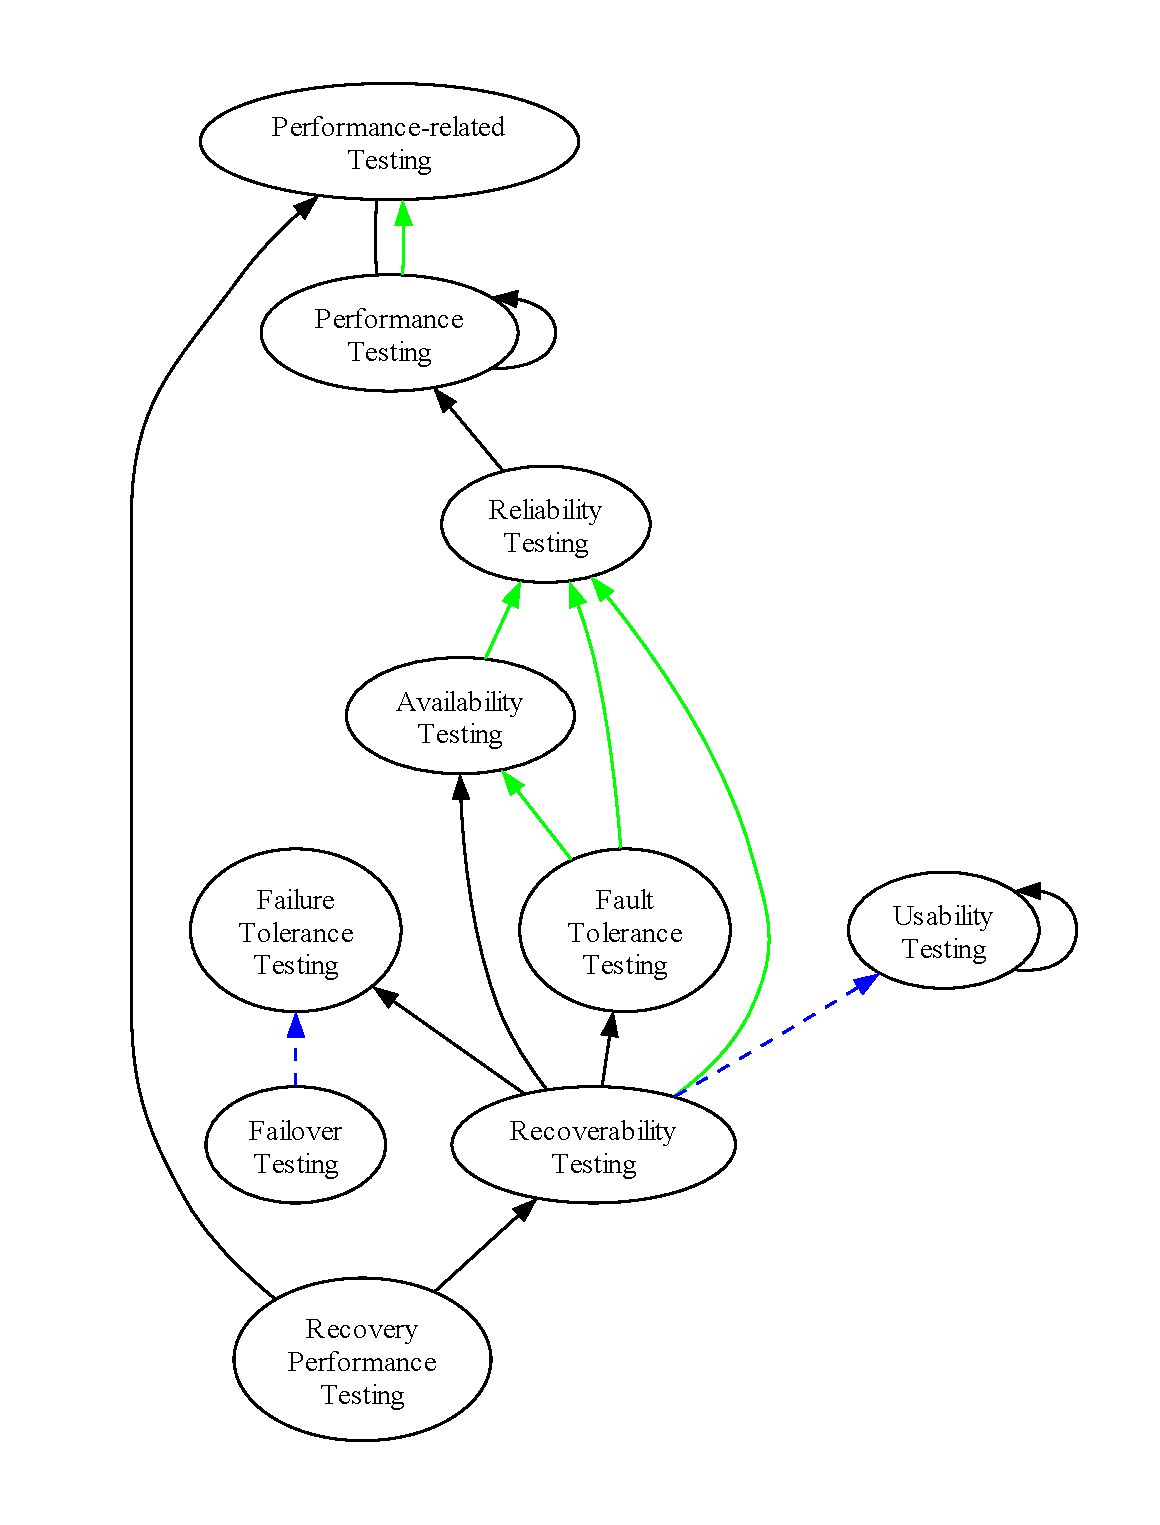
\includegraphics[width=\linewidth]{assets/graphs/recoveryProposedGraph.pdf}
            \caption{Graph of proposed relations.}
            \label{fig:recovery-graph-proposed}
        \end{subfigure}
        \caption{Graphs of relations between terms related to recovery testing.}
        \label{fig:recoveryGraphs}
    \end{figure}
}

\newcommand{\scalGraphs}{
    % Only top or bottom to comply with IEEE guidelines
    \begin{figure}[bt!]
        \centering
        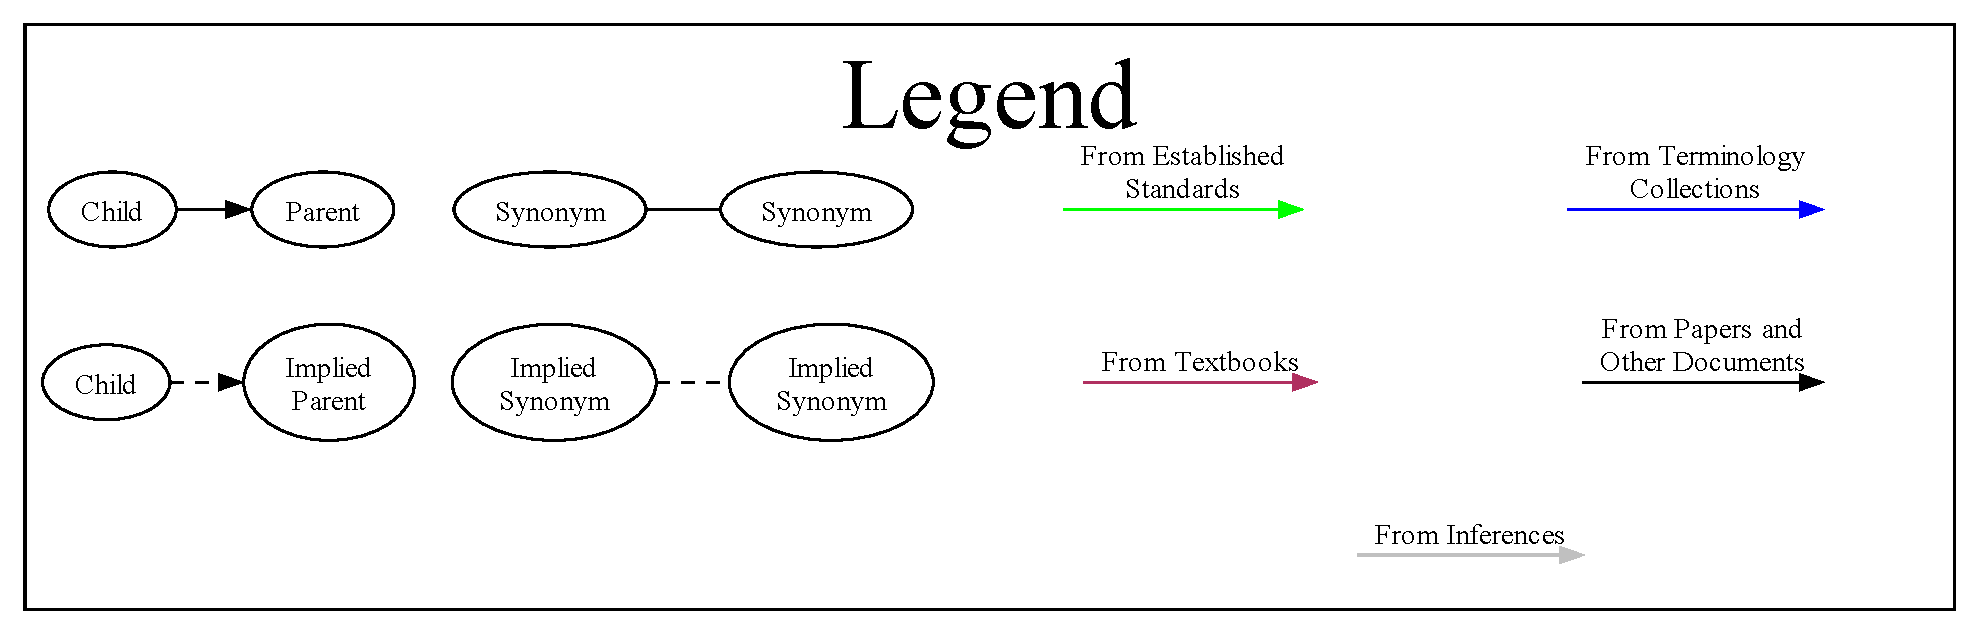
\includegraphics[width=\linewidth]{assets/graphs/scalabilityLegend.pdf}
        \begin{subfigure}[b]{.475\linewidth}
            \centering
            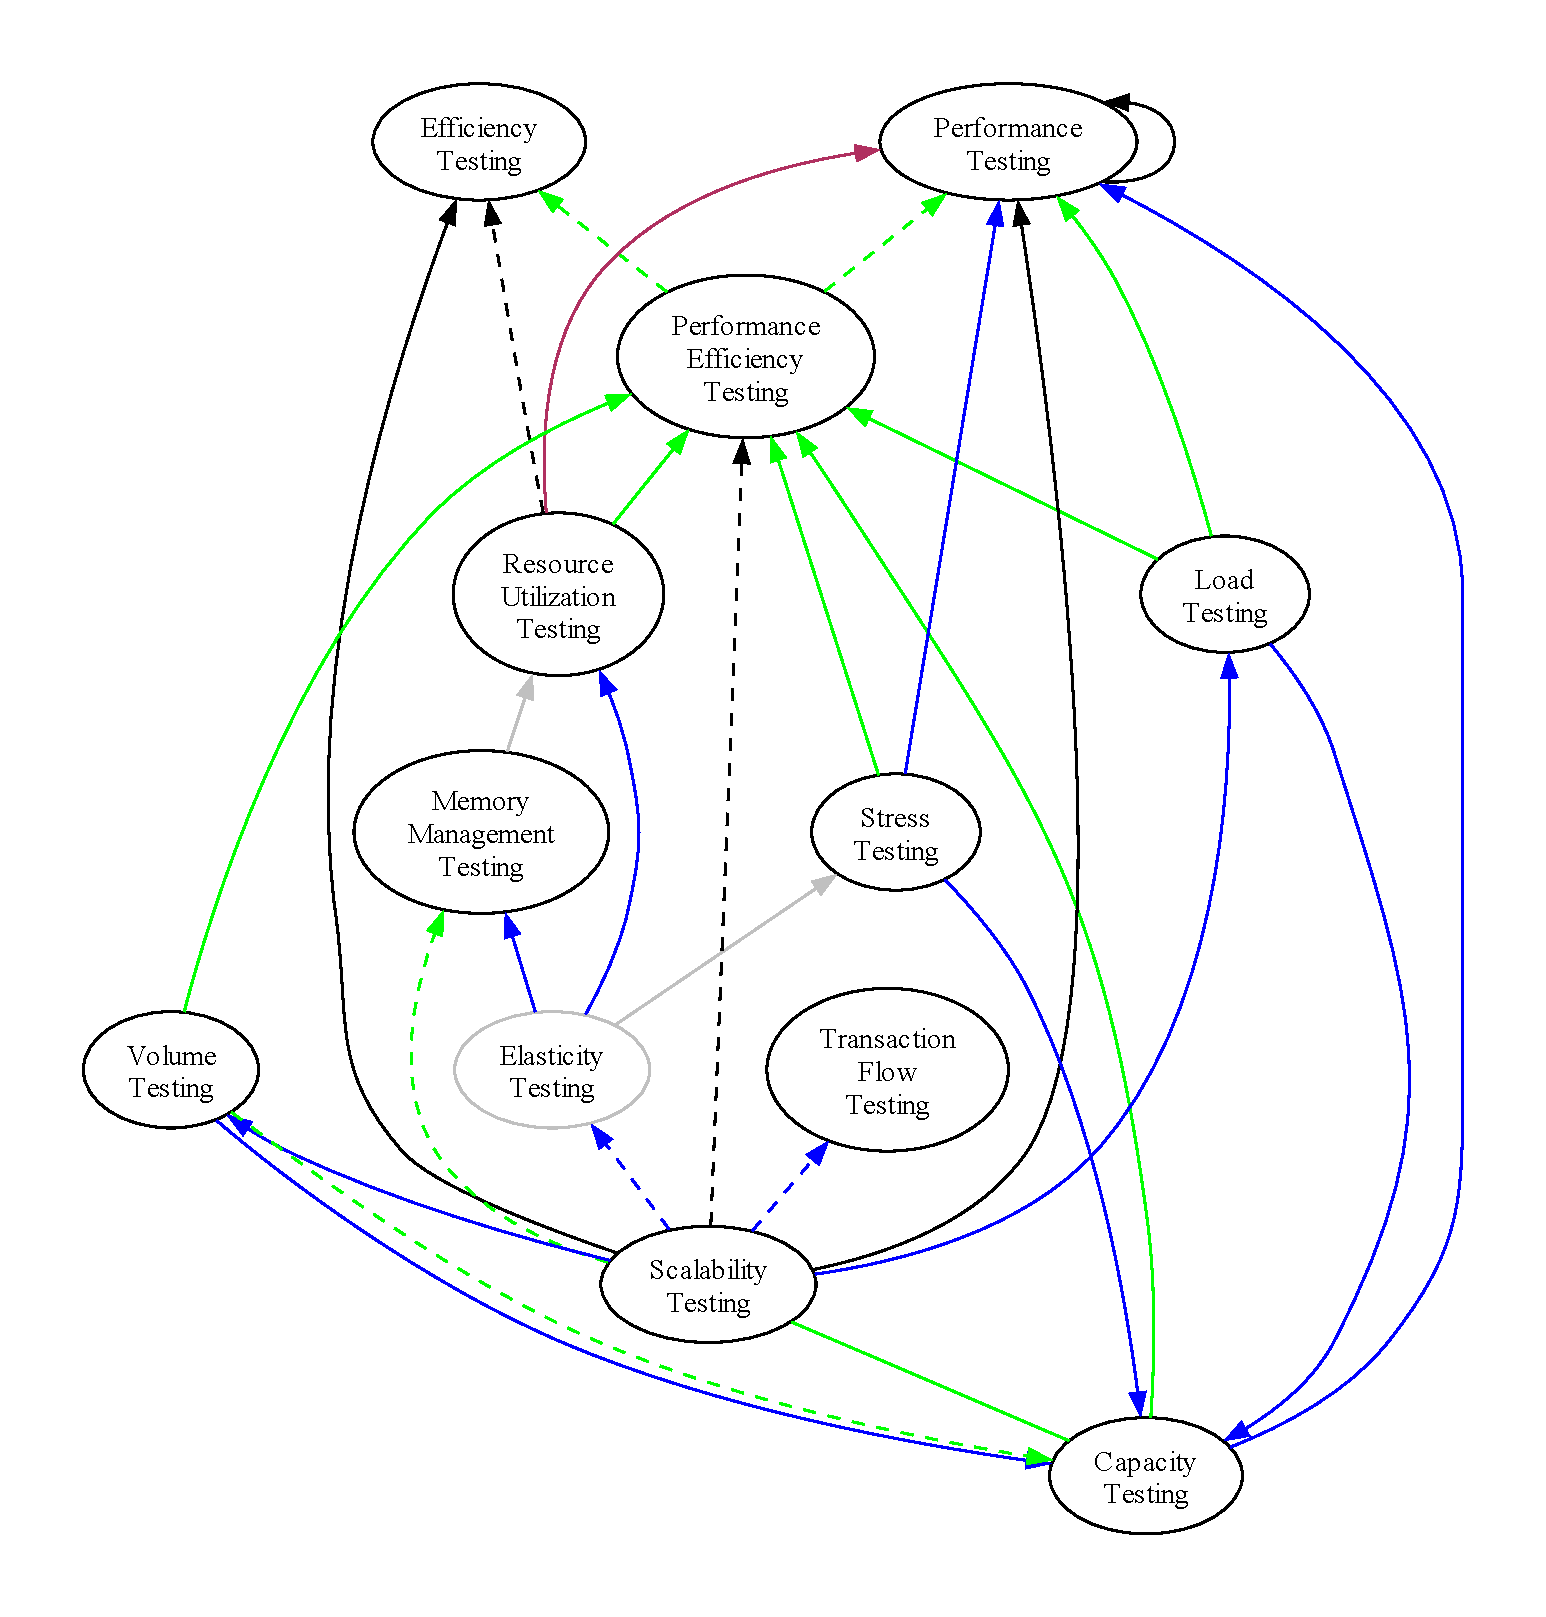
\includegraphics[width=\linewidth]{assets/graphs/scalabilityGraph.pdf}
            \caption{Graph of current relations.}
            \label{fig:scal-graph-current}
        \end{subfigure}
        \begin{subfigure}[b]{.475\linewidth}
            \centering
            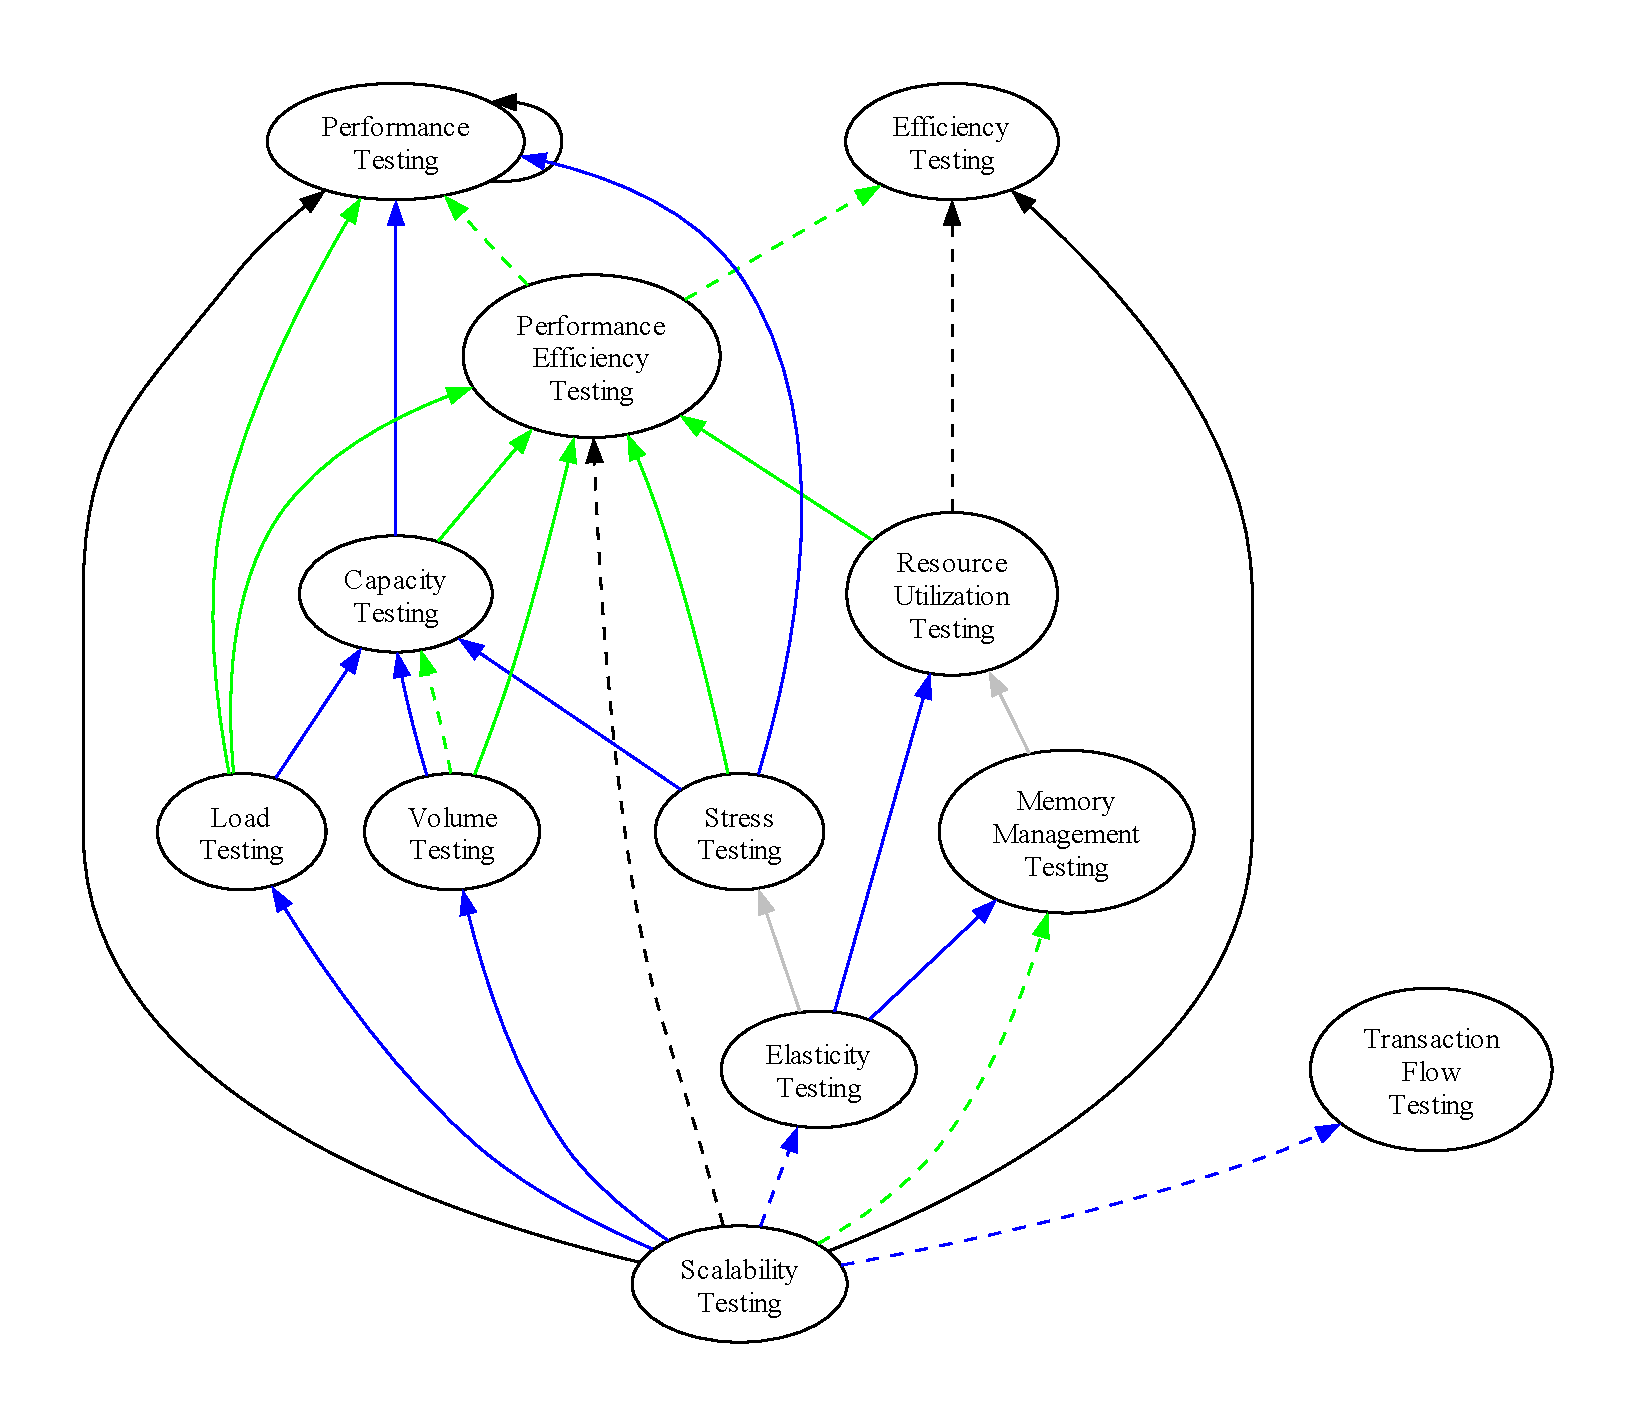
\includegraphics[width=\linewidth]{assets/graphs/scalabilityProposedGraph.pdf}
            \caption{Graph of proposed \ifnotpaper \else \\ \fi relations.}
            \label{fig:scal-graph-proposed}
        \end{subfigure}
        \caption{Graphs of relations between terms related to scalability testing.}
        \label{fig:scalGraphs}
    \end{figure}
}

\newcommand{\performanceGraph}{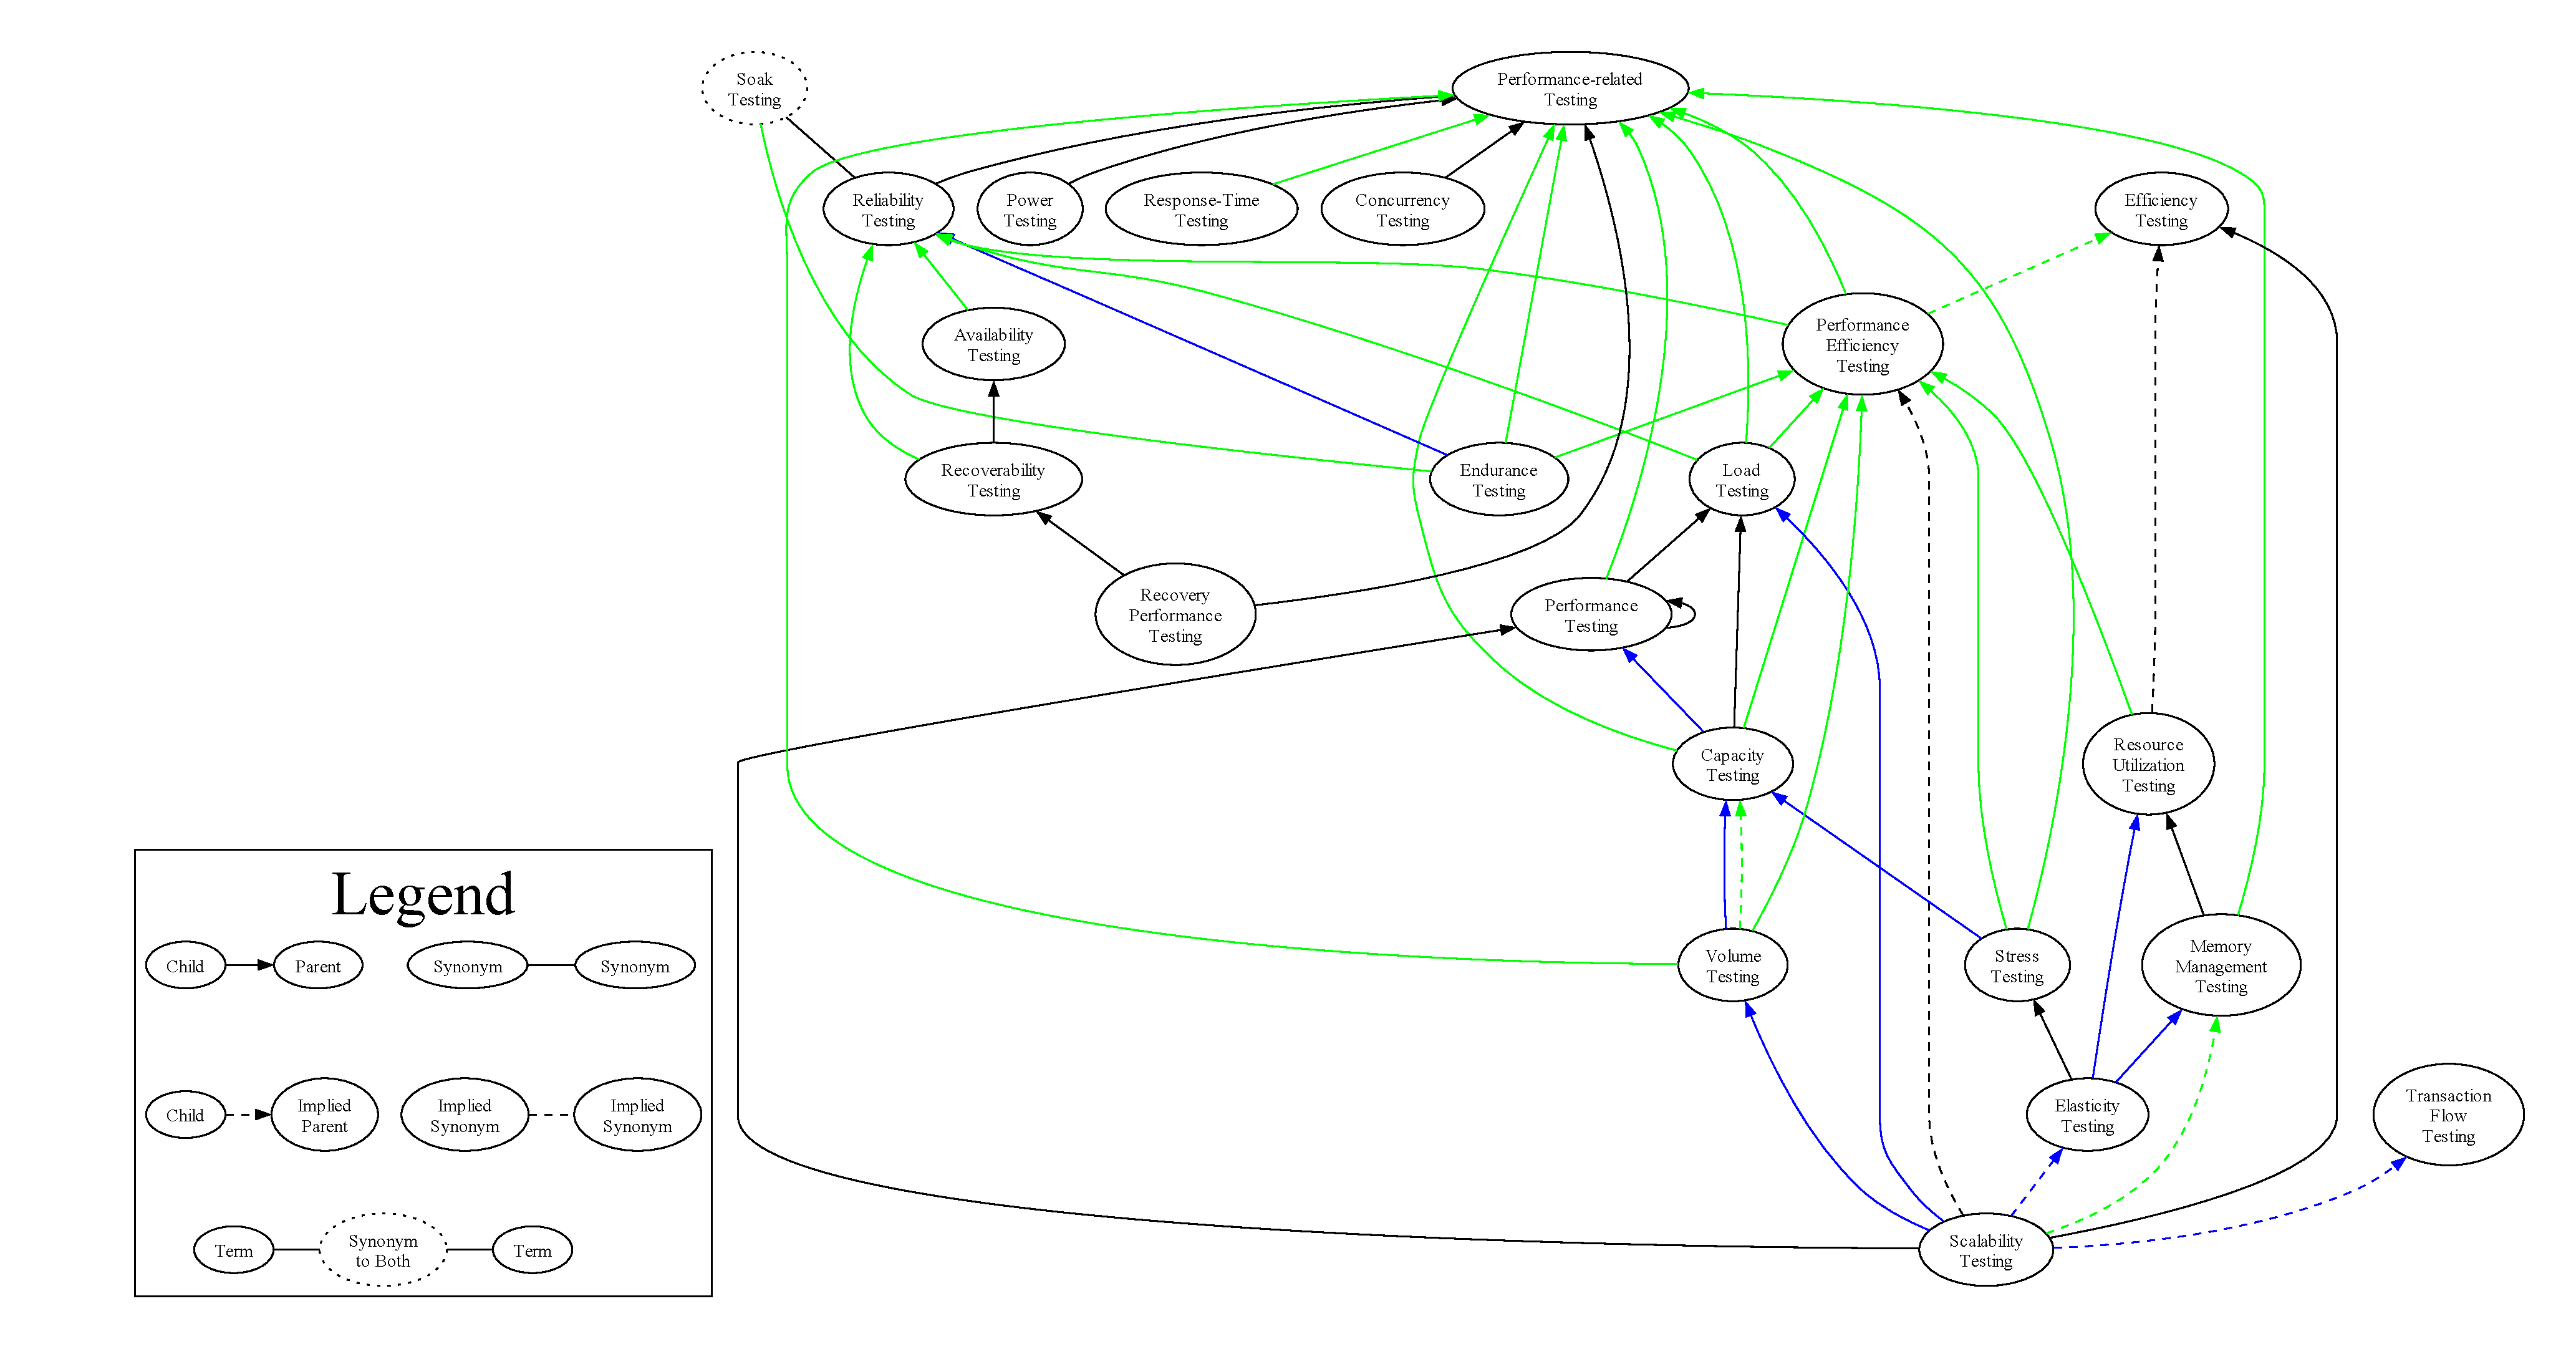
\includegraphics[width=\linewidth]{assets/graphs/performanceProposedGraph.pdf}}

%------------------------------------------------------------------------------
% Images & Figures
%------------------------------------------------------------------------------

\newcommand{\drasilLogo}{assets/images/drasil_logo.png}
\newcommand{\drasilLogoImg}{\begin{figure}[H]
    \centering
    \caption{Drasil's Logo}
    \label{fig:drasilLogo}

    \includegraphics[width=0.6\linewidth]{\drasilLogo}
\end{figure}
}
\newcommand{\refDrasilLogoImg}{\Cref{fig:drasilLogo}}

%------------------------------------------------------------------------------
% Tables
%------------------------------------------------------------------------------

% Organization of files
\newcommand{\organizationTable}{\begin{longtable}[c]{|>{\raggedright}p{0.3\linewidth}|>{\raggedright\arraybackslash}p{0.54\linewidth}|}
    \caption{Template Organization}
    \label{tab:organization}                                              \\

    \hline

    \rowcolor{McMasterMediumGrey}
    \textbf{File/Folder}     & \textbf{Intended Usage \& Description}
    \\ \hline

    \texttt{thesis.tex} & Focal \LaTeX{} file that collects everything and is
    used to build your thesis/report document.
    \\ \hline

    \texttt{Makefile} & A basic \texttt{Makefile} configuration. See
    \texttt{make help} for a list of helpful commands. \\ \hline

    \texttt{build/} & When you build your \acs{pdf}, this folder is used as the
    working directory of LuaLaTeX. Using this allows us to quickly get rid of
    \LaTeX{} build files that can cause problems when we re-build documents. \\
    \hline

    \texttt{manifest.tex} & Basic options that you should certainly configure
    according to your needs.
    \\ \hline

    \texttt{chapters.tex} & All chapters of your thesis should be included here.
    \\ \hline

    \texttt{chapters/} & Enumeration of the chapters of your thesis. I prefer
    using a two-digit indexing pattern for the prefix of file names so that I
    can quickly open up by chapter number using VS Codium. \\ \hline

    \texttt{assets.tex} & Enumeration of the various kinds of ``assets'' in the
    \texttt{assets/} folder. See the file for examples on how you can write your
    extra utility macros. \\ \hline

    \texttt{assets/} & Enumeration of various kinds of ``assets,'' with
    subdirectories for images and figures, tables, and code snippets. \\ \hline

    \texttt{front.tex} & All front matter of your thesis should be included
    here. \\ \hline

    \texttt{front/} & Enumeration of the front chapters of your thesis. These
    chapters should all be numbered using Roman numerals. \\ \hline

    \texttt{back.tex} & All back matter of your thesis should be included here.
    \\ \hline

    \texttt{back/} & Enumeration of the back matter content.
    \\ \hline

    \texttt{acronyms.tex} & List of acronyms you intend to use in your thesis.
    This uses the ``acro'' \LaTeX{} package.
    \\ \hline

    \texttt{macros.tex} & Helpful macros!
    \\ \hline

    \texttt{unicode\_chars.tex} & At times, you might find issues with unicode
    characters, especially in verbatim environments, where you might need to
    manually define them using other font glyphs.
    \\ \hline

    \texttt{mcmaster\_colours.tex} & Macros for the McMaster colour palette.
    \\ \hline

    \texttt{README.md} & Read it!
    \\ \hline

    \texttt{.gitignore} & List of files in the working directory that should be
    ignored by git.
    \\ \hline

    \texttt{latexmkrc} & Used for setting the timezone for latexmk, but can be
    used for other options.
    \\ \hline
\end{longtable}
}

\newcommand{\ieeeCatsTable}{% Conversion to longtblr assisted by GitHub Copilot

\begin{longtblr}[
    note{a} = {Also called ``test phase'' \ifnotpaper (see
            \discrepref{level-phase-syns}) \fi or ``test stage'' \ifnotpaper
            (see \discrepref{stage-level-syns})\else (see relevant synonym
            discrepancies in \Cref{syns})\fi.},
    note{b} = {Also called ``test design technique'' \ifnotpaper
            (\citealp[p.~11]{IEEE2022}; \citealpISTQB{})\else
            \cite[p.~11]{IEEE2022}, \cite{ISTQB}\fi.},
    caption={Categories of testing given by ISO/IEC and IEEE.},
    label={tab:ieeeCats}
    ]{
    colspec={|X[0.09,c,m]X[0.56,m]X[0.3,m]|},
    width = \linewidth, rowhead = 1, hlines
    }
    \thead{Term}                   & \thead{Definition}                           & \thead{Examples} \\
    Test Approach                  & A ``high-level test implementation choice''
    that includes ``test level, test type, test technique, test practice and
    \dots{} static testing'' \citep[p.~10]{IEEE2022} and is used to ``pick the
    particular test case values''
    \citeyearpar[p.~465]{IEEE2017} & black or white box, minimum and maximum
    boundary value testing \citep[p.~465]{IEEE2017}                                                  \\

    Test Level\TblrNote{a}         & A stage of testing ``typically associated
    with the achievement of particular objectives and used to treat particular
    risks'', each performed in sequence \ifnotpaper (\citealp[p.~12]{IEEE2022};
    \citeyear[p.~6]{IEEE2021}) \else \cite[p.~12]{IEEE2022}, \cite[p.~6]{IEEE2021}
    \fi with their ``own documentation and resources''
    \citeyearpar[p.~469]{IEEE2017} % ; more generally, ``designat[es] \dots\ the
    % coverage and detail'' \citeyearpar[p.~249]{IEEE2017} 
                                   & unit/component testing, integration testing,
    system testing, acceptance testing \ifnotpaper (\citealp[p.~12]{IEEE2022};
    \citeyear[p.~6]{IEEE2021}; \citeyear[p.~467]{IEEE2017}) \else
    \cite[p.~12]{IEEE2022}, \cite[p.~467]{IEEE2017}, \cite[p.~6]{IEEE2021} \fi                       \\
    Test Practice                  & A ``conceptual framework that can be
    applied to \dots{} [a] test process to facilitate testing'' \ifnotpaper
    (\citealp[p.~14]{IEEE2022}; \citeyear[p.~471]{IEEE2017}; OG IEEE 2013)
    \else \cite[p.~14]{IEEE2022}, \cite[p.~471]{IEEE2017}
    \fi % ; more generally, a ``specific type of activity that contributes to
    % the execution of a process'' \citeyearpar[p.~331]{IEEE2017} 
                                   & scripted testing, exploratory testing,
    automated testing \citep[p.~20]{IEEE2022}                                                        \\
    Test Technique\TblrNote{b}     & A ``procedure used to create or select a
    test model, identify test coverage items, and derive corresponding test
    cases'' \ifnotpaper (\citeyear[p.~11]{IEEE2022}; similar in
    \citeyear[p.~467]{IEEE2017}) \else \cite[p.~11]{IEEE2022} (similar in
    \cite[p.~467]{IEEE2017}) \fi that ``generate evidence that test item
    requirements have been met or that defects are present in a test item''
    \citeyearpar[p.~vii]{IEEE2021} % ; ``a variety \dots\ is typically
    % required to suitably cover any system'' \citeyearpar[p.~33]{IEEE2022} and
    % is ``often selected based on team skills and familiarity, on the format
    % of the test basis'', and on expectations \citeyearpar[p.~23]{IEEE2022}
                                   & equivalence partitioning,
    boundary value analysis, branch testing \citep[p.~11]{IEEE2022}                                  \\
    Test Type                      & ``Testing that is focused on specific
    quality characteristics'' \ifnotpaper (\citealp[p.~15]{IEEE2022};
    \citeyear[p.~7]{IEEE2021}; \citeyear[p.~473]{IEEE2017}; OG IEEE 2013)
    \else \cite[p.~15]{IEEE2022}, \cite[p.~473]{IEEE2017}, \cite[p.~7]{IEEE2021}
    \fi                            & security testing, usability testing,
    performance testing \ifnotpaper (\citealp[p.~15]{IEEE2022};
    \citeyear[p.~473]{IEEE2017}) \else\cite[p.~15]{IEEE2022},
    \cite[p.~473]{IEEE2017} \fi                                                                      \\
\end{longtblr}
}
\newcommand{\otherCatsTable}{% Defined here so VS Code doesn't freak out
\def\ieeeEquiv{\makecell{IEEE\\Equivalent}}
\def\swebokLevel{{Level\\(objective-\\based)\TblrNote{a}}}

\begin{longtblr}[
    note{a} = {See \flawref{stage-level-syns}.},
    note{b} = {Testing methods and guidances are omitted from this table
            since \citet{BarbosaEtAl2006} do not define or give examples of them.},
    note{c} = {Synonyms for these examples are used by
            \citet[p.~3; OG Mathur, 2012]{SouzaEtAl2017} and
            \citet[p.~3]{BarbosaEtAl2006}.},
    caption={Categories of testing given by other sources.},
    label={tab:otherCats}
    ]{
    colspec={|X[0.08,c,m]|X[0.43,m]|X[0.34,m]|Q[c,m]|},
    width = \linewidth, rowhead = 1
    }
    \hline
    \thead{Term}                           & \thead{Definition}           & \thead{Examples} & \thead{\ieeeEquiv{}} \\
    \hline
    % Guidance                               & none given
    % \citep[p.~3]{BarbosaEtAl2006}          & none given         & Technique?                              \\
    \swebokLevel{}                         & Test levels based on the
    purpose of testing \citep[p.~5\=/6]{SWEBOK2024} that ``determine
    how the test suite is identified \dots\ regarding its consistency
    \dots\ and its composition''
    \citetext{p.~5\=/2}                    & conformance testing,
    installation testing, regression testing, performance testing,
    security testing % reliability testing,
    \citep[pp.~5\=/7 to 5\=/9]{SWEBOK2024} & Type?                                                                  \\
    % Method                                 & none given
    % \citep[p.~3]{BarbosaEtAl2006}          & none given         & Practice?                               \\
    Phase                                  & none given
    %(\citealp[p.~221]{Perry2006}; \citealp[p.~3]{BarbosaEtAl2006})  
                                           & unit testing,
    integration testing, system testing, regression testing (\citealp[p.~221]{Perry2006};
    \citealp[p.~3]{BarbosaEtAl2006})       & Level                                                                  \\
    Procedure                              & The basis for how
    testing is performed that guides the process; ``categorized in[to] testing methods,
    testing guidances\TblrNote{b} and testing techniques''
    \citep[p.~3]{BarbosaEtAl2006}          & none given
    generally; see ``Technique''           & Approach                                                               \\
    Process                                & ``A sequence of
    testing steps'' \citep[p.~2]{BarbosaEtAl2006} ``based on a development technology and \dots\
    paradigm, as well as on a testing procedure''
    \citetext{p.~3}                        & none given                   & Practice                                \\
    Stage                                  & An
    alternative to the ``traditional \dots\ test stages'' %\footnote{See ``Level'' in \Cref{tab:ieeeCats}.}
    based on ``clear technical groupings''
    \citep[p.~13]{Gerrard2000a}            & desktop development testing,
    infrastructure testing,
    % system testing, large scale integration, and
    post-deployment monitoring
    \citep[p.~13]{Gerrard2000a}            & Level                                                                  \\
    Technique                              & ``Systematic
    procedures and approaches for generating or selecting the most suitable test suites''
    \citep[p.~5\=/10]{SWEBOK2024}          & specification-based testing,
    % ``on a sound theoretical basis'' \citep[p.~3]{BarbosaEtAl2006}
    structure-based testing, fault-based testing\TblrNote{c}
    % , experience-based testing, usage-based testing
    (\citealp[pp.~5\=/10, 5\=/13 to 5\=/15]{SWEBOK2024})
    % black-box, white-box, defect/fault-based, model-based testing
    % \citetext{\citealp[p.~3]{SouzaEtAl2017}; OG Mathur, 2012};
    % functional, structural, error-based, state-based testing \citep[p.~3]{BarbosaEtAl2006}
                                           & Technique                                                              \\
    \hline
\end{longtblr}
}
\newcommand{\otherCategorizationsTable}{\def\selecExs{Deterministic Testing\\ Random Testing}
\def\covExs{Input Space Partitioning\\ Graph Coverage\\ Logic Coverage\\ Syntax-based Testing}
\def\execExs{Static Testing\\ Dynamic Testing}
\def\goalExs{Verification Testing\\ Validation Testing}
\def\propExs{Functional Testing\\ Non-functional Testing}

\begin{paperTable}
    \centering
    \begin{minipage}{\linewidth}
        \begin{longtblr}[
            note{\textrm{a}} = {We also consider this categorization meaningful (see \Cref{static-test}).},
            note{\textrm{b}} = {Functional testing is categorized ambiguously (see \Cref{func-test-discrep}) and non-functional testing is uncategorized.},
            caption = {Alternate categorizations given by the literature.},
            label = {tab:otherCategorizations}
            ]{
            colspec = {|X[0.35,c,m]X[0.2,c,m]X[0.35,c,m]|}, width = \linewidth,
            rowhead = 1
            }
            \hline
            \thead{Test Basis}                                        & \thead{Example Approaches} & \thead{Subset of}                                                                                                                      \\
            \hline
            Selection Process \citep[p.~5-16]{SWEBOK2024}             & \selecExs{}                & Technique \citep[pp.~5-12, 5-16]{SWEBOK2024}                                                                                           \\
            \hline
            Coverage Criteria \citep[pp.~18--19]{AmmannAndOffutt2017} & \covExs{}                  & Technique (\citealp[p.~22]{IEEE2022}; \citeyear[Fig.~2]{IEEE2021}; \citealp[p.~5-11]{SWEBOK2024}; \citealp[pp.~47--48]{Firesmith2015}) \\
            \hline
            Execution of Code{\MidTblrNote{\textrm{a}}} (\citealp[p.~214]{KuļešovsEtAl2013}; \citealp[p.~12]{Gerrard2000a};
            \citealp[p.~53]{Patton2006})                              & \execExs{}                 & Approach                                                                                                                               \\
            \hline
            Goal of Testing (\citealp[p.~214]{KuļešovsEtAl2013};
            \citealp[pp.~69--70]{Perry2006})                          & \goalExs{}                 & Approach                                                                                                                               \\
            \hline
            Property of Code \citep[p.~213]{KuļešovsEtAl2013}
            or Test Target \citep[pp.~4--5]{Kam2008}                  & \propExs{}                 & Approach\TblrNote{\textrm{b}}                                                                                                          \\
            \hline
        \end{longtblr}
    \end{minipage}
\end{paperTable}
}

\newcommand{\sntxFlawsTable}{\begin{paperTable}
    \centering
    \caption{Breakdown of identified \nameref{sntxFlaws} by \srcCat{}.}
    \label{tab:sntxFlaws}
    \begin{minipage}{\linewidth}
        \begin{tabular}{|r|*{6}{cc|}c|}
            \hline
                              & \multicolumn{2}{c|}{\thead{\nameref{wrong}}} & \multicolumn{2}{c|}{\thead{\nameref{miss}}} & \multicolumn{2}{c|}{\thead{\nameref{contra}}} & \multicolumn{2}{c|}{\thead{\nameref{ambi}}} & \multicolumn{2}{c|}{\thead{\nameref{over}}} & \multicolumn{2}{c|}{\thead{\reduns{}}} &                                                                                                                                                                                         \\
            \thead{\srcCat{}} & \thead{Exp}                                  & \thead{Imp}                                 & \thead{Exp}                                   & \thead{Imp}                                 & \thead{Exp}                                 & \thead{Imp}                            & \thead{Exp}             & \thead{Imp}             & \thead{Exp}             & \thead{Imp}              & \thead{Exp}              & \thead{Imp}              & \thead{Total}            \\
            \hline
            \stds{}           & \stdSntxFlawBrkdwn{1}                        & \stdSntxFlawBrkdwn{2}                       & \stdSntxFlawBrkdwn{3}                         & \stdSntxFlawBrkdwn{4}                       & \stdSntxFlawBrkdwn{5}                       & \stdSntxFlawBrkdwn{6}                  & \stdSntxFlawBrkdwn{7}   & \stdSntxFlawBrkdwn{8}   & \stdSntxFlawBrkdwn{9}   & \stdSntxFlawBrkdwn{10}   & \stdSntxFlawBrkdwn{11}   & \stdSntxFlawBrkdwn{12}   & \stdSntxFlawBrkdwn{13}   \\
            \metas{}          & \metaSntxFlawBrkdwn{1}                       & \metaSntxFlawBrkdwn{2}                      & \metaSntxFlawBrkdwn{3}                        & \metaSntxFlawBrkdwn{4}                      & \metaSntxFlawBrkdwn{5}                      & \metaSntxFlawBrkdwn{6}                 & \metaSntxFlawBrkdwn{7}  & \metaSntxFlawBrkdwn{8}  & \metaSntxFlawBrkdwn{9}  & \metaSntxFlawBrkdwn{10}  & \metaSntxFlawBrkdwn{11}  & \metaSntxFlawBrkdwn{12}  & \metaSntxFlawBrkdwn{13}  \\
            \texts{}          & \textSntxFlawBrkdwn{1}                       & \textSntxFlawBrkdwn{2}                      & \textSntxFlawBrkdwn{3}                        & \textSntxFlawBrkdwn{4}                      & \textSntxFlawBrkdwn{5}                      & \textSntxFlawBrkdwn{6}                 & \textSntxFlawBrkdwn{7}  & \textSntxFlawBrkdwn{8}  & \textSntxFlawBrkdwn{9}  & \textSntxFlawBrkdwn{10}  & \textSntxFlawBrkdwn{11}  & \textSntxFlawBrkdwn{12}  & \textSntxFlawBrkdwn{13}  \\
            \papersTbl{}      & \paperSntxFlawBrkdwn{1}                      & \paperSntxFlawBrkdwn{2}                     & \paperSntxFlawBrkdwn{3}                       & \paperSntxFlawBrkdwn{4}                     & \paperSntxFlawBrkdwn{5}                     & \paperSntxFlawBrkdwn{6}                & \paperSntxFlawBrkdwn{7} & \paperSntxFlawBrkdwn{8} & \paperSntxFlawBrkdwn{9} & \paperSntxFlawBrkdwn{10} & \paperSntxFlawBrkdwn{11} & \paperSntxFlawBrkdwn{12} & \paperSntxFlawBrkdwn{13} \\
            \hline
            Total             & \totalSntxFlawBrkdwn{1}                      & \totalSntxFlawBrkdwn{2}                     & \totalSntxFlawBrkdwn{3}                       & \totalSntxFlawBrkdwn{4}                     & \totalSntxFlawBrkdwn{5}                     & \totalSntxFlawBrkdwn{6}                & \totalSntxFlawBrkdwn{7} & \totalSntxFlawBrkdwn{8} & \totalSntxFlawBrkdwn{9} & \totalSntxFlawBrkdwn{10} & \totalSntxFlawBrkdwn{11} & \totalSntxFlawBrkdwn{12} & \totalSntxFlawBrkdwn{13} \\
            \hline
        \end{tabular}
    \end{minipage}
\end{paperTable}
}
\newcommand{\smntcFlawsTable}{\begin{paperTable}
    \centering
    \caption{Breakdown of identified \nameref{smntcFlaws} by \srcCat{}.}
    \label{tab:smntcFlaws}
    % \begin{minipage}{\linewidth}
    \begin{tabular}{|r|*{6}{cc|}c|}
        \hline
                          & \multicolumn{2}{c|}{\thead{\cats{}}} & \multicolumn{2}{c|}{\thead{\syns{}}} & \multicolumn{2}{c|}{\thead{\pars{}}} & \multicolumn{2}{c|}{\thead{\defs{}}} & \multicolumn{2}{c|}{\thead{\terms{}}} & \multicolumn{2}{c|}{\thead{\cites{}}} &                                                                                                                                                                                                \\
        % \cline{2-10}
        \thead{\srcCat{}} & \thead{Exp}                          & \thead{Imp}                          & \thead{Exp}                          & \thead{Imp}                          & \thead{Exp}                           & \thead{Imp}                           & \thead{Exp}              & \thead{Imp}              & \thead{Exp}              & \thead{Imp}               & \thead{Exp}               & \thead{Imp}               & \thead{Total}             \\
        \hline
        \stds{}           & \stdSmntcFlawBrkdwn{1}               & \stdSmntcFlawBrkdwn{2}               & \stdSmntcFlawBrkdwn{3}               & \stdSmntcFlawBrkdwn{4}               & \stdSmntcFlawBrkdwn{5}                & \stdSmntcFlawBrkdwn{6}                & \stdSmntcFlawBrkdwn{7}   & \stdSmntcFlawBrkdwn{8}   & \stdSmntcFlawBrkdwn{9}   & \stdSmntcFlawBrkdwn{10}   & \stdSmntcFlawBrkdwn{11}   & \stdSmntcFlawBrkdwn{12}   & \stdSmntcFlawBrkdwn{13}   \\
        \metas{}          & \metaSmntcFlawBrkdwn{1}              & \metaSmntcFlawBrkdwn{2}              & \metaSmntcFlawBrkdwn{3}              & \metaSmntcFlawBrkdwn{4}              & \metaSmntcFlawBrkdwn{5}               & \metaSmntcFlawBrkdwn{6}               & \metaSmntcFlawBrkdwn{7}  & \metaSmntcFlawBrkdwn{8}  & \metaSmntcFlawBrkdwn{9}  & \metaSmntcFlawBrkdwn{10}  & \metaSmntcFlawBrkdwn{11}  & \metaSmntcFlawBrkdwn{12}  & \metaSmntcFlawBrkdwn{13}  \\
        \texts{}          & \textSmntcFlawBrkdwn{1}              & \textSmntcFlawBrkdwn{2}              & \textSmntcFlawBrkdwn{3}              & \textSmntcFlawBrkdwn{4}              & \textSmntcFlawBrkdwn{5}               & \textSmntcFlawBrkdwn{6}               & \textSmntcFlawBrkdwn{7}  & \textSmntcFlawBrkdwn{8}  & \textSmntcFlawBrkdwn{9}  & \textSmntcFlawBrkdwn{10}  & \textSmntcFlawBrkdwn{11}  & \textSmntcFlawBrkdwn{12}  & \textSmntcFlawBrkdwn{13}  \\
        \papersTbl{}      & \paperSmntcFlawBrkdwn{1}             & \paperSmntcFlawBrkdwn{2}             & \paperSmntcFlawBrkdwn{3}             & \paperSmntcFlawBrkdwn{4}             & \paperSmntcFlawBrkdwn{5}              & \paperSmntcFlawBrkdwn{6}              & \paperSmntcFlawBrkdwn{7} & \paperSmntcFlawBrkdwn{8} & \paperSmntcFlawBrkdwn{9} & \paperSmntcFlawBrkdwn{10} & \paperSmntcFlawBrkdwn{11} & \paperSmntcFlawBrkdwn{12} & \paperSmntcFlawBrkdwn{13} \\
        \hline
        Total             & \totalSmntcFlawBrkdwn{1}             & \totalSmntcFlawBrkdwn{2}             & \totalSmntcFlawBrkdwn{3}             & \totalSmntcFlawBrkdwn{4}             & \totalSmntcFlawBrkdwn{5}              & \totalSmntcFlawBrkdwn{6}              & \totalSmntcFlawBrkdwn{7} & \totalSmntcFlawBrkdwn{8} & \totalSmntcFlawBrkdwn{9} & \totalSmntcFlawBrkdwn{10} & \totalSmntcFlawBrkdwn{11} & \totalSmntcFlawBrkdwn{12} & \totalSmntcFlawBrkdwn{13} \\
        \hline
    \end{tabular}
    % \end{minipage}
\end{paperTable}}

\newcommand{\testReqsTable}{% To prevent VSCode from aligning things weirdly
\def\typeHead{Testing\\Approach}

\begin{table}[hbtp!]
    \centering
    \caption{Testing Requirements}
    \label{tab:testReqs}
    \begin{tabularx}{\textwidth}{|p{0.14\textwidth}|X|c|c|}
        \hline
        \rowcolor{McMasterMediumGrey}
        \thead{\typeHead}       & \thead{Requirements}                         & \thead{In Drasil?} & \thead{Addable?} \\
        \hline
        Unit testing            & Code modules and their specifications        & ??                 & ??               \\
        Integration testing     & Code modules and their interfaces            & ??                 & ??               \\
        System testing          & Requirements specification; most of the code
                                & ??                                           & ??                                    \\
        Acceptance testing      & Customer requirements and feedback           & ??                 & ??               \\
        Installation testing    & Algorithm for installation; environments to
        test in; method to check
        successful installation & ??                                           & ??                                    \\
        \hline
    \end{tabularx}
\end{table}}


% McMaster Colours
% -- McMaster Colours --

% McMaster Palette based on https://brand.mcmaster.ca/element/colour-palette/

% Heritage Colours
\definecolor{McMasterHeritageMaroon}{HTML}{7A003C}
\definecolor{McMasterHeritageGold}{HTML}{FDBF57}
\definecolor{McMasterHeritageGrey}{HTML}{5E6A71}

% Tints and Shades
\definecolor{McMasterLightMaroon}{HTML}{ac1455}
\definecolor{McMasterDarkMaroon}{HTML}{56002a}

\definecolor{McMasterLightGrey}{HTML}{efefef}
\definecolor{McMasterCoolGrey}{HTML}{dbdbdd}
\definecolor{McMasterMediumGrey}{HTML}{aeb4b8}
\definecolor{McMasterDarkGrey}{HTML}{222222}

% Highlights
\definecolor{McMasterWorldYellow}{HTML}{FFD100}
\definecolor{McMasterWorldLime}{HTML}{D2D755}
\definecolor{McMasterWorldSkyBlue}{HTML}{8BD3E6}

% Darker Tones
\definecolor{McMasterWorldRed}{HTML}{A6192E}
\definecolor{McMasterWorldGreen}{HTML}{007B4B}
\definecolor{McMasterWorldBlue}{HTML}{007096}


% For fancy pictures
\usepackage{tikz}
\usetikzlibrary{shapes,arrows,cd,babel,arrows.meta,graphs,graphdrawing}
\usegdlibrary {layered}

% Make sure the floating lists (figures, source codes, and abbreviations) are
% shown in the toc.
\usepackage{tocbibind}

% Counters
\usepackage{chngcntr}

\title{
    {\thesisTitle{}}\\
    {\thesisInstitution{}}
}
\author{\thesisAuthorName{}}
\date{\thesisSubmissionMonthYear{}}

% START : TODO LIST SETUP
\ifshowwritingdirectives
  \usepackage[backgroundcolor=yellow,colorinlistoftodos]{todonotes}
  \setlength{\marginparwidth}{\thesisTODOMarginSize{}}
  \reversemarginpar % place on left-hand side
\else
  \usepackage[disable]{todonotes}
\fi
% END   : TODO LIST SETUP

\begin{document}

%------------------------------------------------------------------------------
% Front Matters
%------------------------------------------------------------------------------

\frontmatter

% START : TODO LIST
% Only show it if the "show writing directives" flag is enabled
\ifshowwritingdirectives
  \todototoc
  \listoftodos
  \newpage
\fi
% END   : TODO LIST

%------------------------------------------------------------------------------
% Half Title page
%------------------------------------------------------------------------------

% First two pages will have a slightly different margin than the rest of the
% document, for the sake of making the document look slightly nicer.
\newgeometry{margin=1in}

\pagenumbering{gobble} % page 0
\null % Needed or else vspace doesn't work
\vspace{0.25\textheight}

\begin{center}
  \MakeUppercase{\thesisHalfTitle}
\end{center}

\newpage

%------------------------------------------------------------------------------
% Title page
%------------------------------------------------------------------------------

\null % Needed, or else vspace doesn't work
\begin{center}
  \vfill
  {\Large{\MakeUppercase{\thesisTitle}}}

  \vfill

  By \MakeUppercase{\thesisAuthorName}, \thesisAuthorCredentials{}

  \vfill

  \textsc{
  A \thesisType{}\\
  Submitted to the \thesisInstitutionDepartment{}\\
  and the \thesisInstitutionGraduateStudies{}\\
  of \thesisInstitution{}\\
  in Partial Fulfillment of the Requirements\\
  for the Degree of\\
  \thesisTargetDegreeName{}}  
  
  \vfill

  \thesisInstitution{} \textcopyright{} Copyright by \thesisAuthorName{}, \thesisSubmissionMonthYear{}

\end{center}

\newpage

% restore the required margin details for the rest of the document.
\restoregeometry

% START : HEADER %
\pagestyle{fancy}
\fancyhead{}
\fancyfoot{}
\fancyfoot[C]{\thepage}
\renewcommand{\headrulewidth}{0pt} % Remove underline of header
% END   : HEADER %

%------------------------------------------------------------------------------
% Descriptive Note
%------------------------------------------------------------------------------

\pagenumbering{roman}
\setcounter{page}{2} % page 2
\noindent
\thesisTargetDegreeName{} (\thesisSubmissionYear{}) \hfill \thesisInstitution{} \\
(\thesisInstitutionDepartment{})                    \hfill \thesisCityProvince{}

\vspace{2cm}

\noindent
\begin{flushleft}
    \begin{tabular}{@{}ll}
        TITLE:      & \thesisTitle{}                                                  \\
        AUTHOR:     & \thesisAuthorName{}, \thesisAuthorCredentials{}                 \\
        SUPERVISOR: & \thesisSupervisor{}                                             \\
        PAGES:      & \pageref{\thesisLastPageOfFrontMatterLabel}, \pageref{LastPage}
    \end{tabular}
\end{flushleft}

\newpage

%------------------------------------------------------------------------------
% Lay Abstract
%------------------------------------------------------------------------------

\chapter{Lay Abstract}
\label{chap:lay_abstract}

\imptodo{Lay abstract.}


%------------------------------------------------------------------------------
% Abstract
%------------------------------------------------------------------------------

\chapter{Abstract}
\label{abstract}%
Testing is a pervasive software development activity that is often
complicated and expensive (if not simply overlooked), partly due to
the lack of a standardized and consistent taxonomy for software testing.
This hinders precise communication, leading to discrepancies across the
literature and even within individual documents!
% Therefore, automating the software testing process is an area of interest,
% and understanding the underlying domain is an important prerequisite.
In this paper, we systematically examine the current state of software
testing terminology. We 1) identify established standards
and prominent testing resources, 2) capture relevant testing terms
from these sources, along with their definitions and relationships---both
explicit and implicit---and 3) construct graphs to visualize and analyze
this data. Our research uncovered \approachCount{} test approaches and
four in-scope methods for describing ``implied'' test approaches. We also build
a tool for generating graphs that illustrate relations between test
approaches and track discrepancies captured by this tool and manually through
the research process. Our results reveal \totalDiscreps{} discrepancies,
including ten terms used as synonyms to two (or more)
disjoint test approaches and \parSynCount{} pairs of test approaches may
either be synonyms or have a parent-child relationship. They also reveal
notable confusion surrounding functional, operational acceptance, recovery,
and scalability testing. These findings make clear
the urgent need for improved testing terminology so that the discussion,
analysis and implementation of various test approaches can be more coherent.
We provide some preliminary advice on how to achieve this standardization.

%------------------------------------------------------------------------------
% Acknowledgements
%------------------------------------------------------------------------------

\chapter{Acknowledgements}
\label{acknowledgements}

ChatGPT was used for assistance with \LaTeX{} formatting and
supplementary Python code for constructing graphs and generating \LaTeX{} code,
including regex. ChatGPT and ProWritingAid were both used for proofreading.
\ifblind{[Additional acknowledgement suppressed.]}{Jason Balaci's
    \href{https://github.com/balacij/McMaster-Thesis-Template}
    {McMaster thesis template} provided many helper \LaTeX{} functions.
    Finally, \supersAck{}.}

%------------------------------------------------------------------------------
% Table of Content
%------------------------------------------------------------------------------

\tableofcontents

%------------------------------------------------------------------------------
% List of Figures
%------------------------------------------------------------------------------

% \renewcommand{\listfigurename}{List of Illustrations, Charts, and Diagrams}
\listoffigures

%------------------------------------------------------------------------------
% List of Tables
%------------------------------------------------------------------------------

\listoftables

%------------------------------------------------------------------------------
% Table of Source Codes
%------------------------------------------------------------------------------

\listoflistings

%------------------------------------------------------------------------------
% List of Abbreviations and Symbols
%------------------------------------------------------------------------------

\printacronyms[
  display=used, % Change value 'used' to 'all' if you want to show unused acronyms
  template=longtable,
  heading=chapter,
  name=List of Abbreviations and Symbols,
  exclude={dupe}
]

%------------------------------------------------------------------------------
% Reading Notes
%------------------------------------------------------------------------------

\chapter{Reading Notes}
\label{chap:reading_notes}

Before reading this thesis, I encourage you to read through these notes, keeping
them in mind while reading.

\begin{itemize}

      \item The source code of this thesis is \porthref{publicly
            available}{https://github.com/balacij/McMaster-Thesis-Template}.

      \item This thesis template is primarily intended for usage by the computer
            science community\footnote{Hence why there are some \LaTeX{} macros
            for ``code'' snippets.}. However, anyone is free to use it.

      \item I've tried my best to make this template conform to the thesis
            requirements as per \porthref{those set forth in 2021 by McMaster
            University}{https://gs.mcmaster.ca/app/uploads/2019/10/Prep_Guide_Masters_and_Doctoral_Theses_August-2021.pdf}.
            However, you should double-check that your usage of this template is
            compliant with whatever the ``current'' rules are.

\end{itemize}

\imptodo{Replace reading notes.}


%------------------------------------------------------------------------------
% Declaration of Academic Achievement
%------------------------------------------------------------------------------

\chapter{Declaration of Academic Achievement}
\label{decl_aca_ach}

This research and analysis was performed by Samuel Crawford under the
guidance, supervision, and recommendations of \supers{}. The resulting
contributions are three glossaries---one for
each of test approaches, software qualities (see \Cref{qual-test}), and
supplementary terms---as well as the tools for data visualization and
automated analysis outlined in \Cref{tools}. These are all available on
\href{https://github.com/samm82/TestingTesting}{an open-source repo}
for independent analysis and, ideally, extension as more test approaches are
discovered and documented.



%------------------------------------------------------------------------------
% Main Matters/Chapters
%------------------------------------------------------------------------------

\mainmatter

% START : HEADER %
\fancyhead[R]{\thesisInstitution{} \textemdash{} \thesisInstitutionDepartmentShort{}}
\fancyhead[L]{\thesisTargetDegreeNameShort{} Thesis \textemdash{} \thesisAuthorNameShort{}}
% END   : HEADER %

\begin{levelup}
    \section{Introduction}

% TODO: tighten up, add sources

Testing software is complicated, expensive, and often overlooked. The
productivity of testing and testing research would benefit from a standard
language for communication. For example, \citet[p.~7]{KanerEtAl2011}
\multAuthHelper{give} the example of complete testing, which could require the
tester to discover ``every bug in the product'', exhaust the time allocated to
the testing phase, or simply implement every test previously agreed upon.
% They go on to say that
Having a clear  definition for ``complete testing'' reduces the chance for
miscommunication and, ultimately, the tester getting ``blamed for not
doing \dots{} [their] job'' \citep[p.~7]{KanerEtAl2011}. These benefits can be
extrapolated to software testing terminology as a whole. Unfortunately, a
search for a systematic, rigorous, and ``complete'' taxonomy for software
testing revealed that the existing ones are inadequate:

\begin{itemize}
    \item \ifnotpaper\else Tebes et al. \fi\citet{TebesEtAl2020a} focus on
          \emph{parts} of the testing process (e.g., test goal, testable entity),
    \item \ifnotpaper\else Souza et al. \fi\citet{SouzaEtAl2017} prioritize
          organizing testing approaches over defining them, and
    \item \ifnotpaper\else Unterkalmsteiner et al. \fi\citet{UnterkalmsteinerEtAl2014}
          focus on the ``information linkage or transfer'' \citetext{p.~A:6}
          between requirements engineering and software testing.
\end{itemize}

\ifnotpaper
    Some existing collections of software testing terminology were found, but
    in addition to being incomplete, they also contained many oversights. For
    example, \citep{IEEE2017} provides the following incomplete/nonsensical
    definitions for the following terms:
    \begin{enumerate}
        \item \textbf{Event Sequence Analysis:} ``per'' \citetext{p.~170}
        \item \textbf{Operable:} ``state of'' \citetext{p.~301}
              % This may be a bad example, since the cf. provides some more context
              % \item \textbf{Software Element:} a ``system element that is software''
              %       \citetext{p.~421}
    \end{enumerate}
    Additionally, it also defines ``device'' as a ``mechanism or piece of
    equipment designed to serve a purpose or perform a function''
    \citetext{p.~136}, but does not define ``equipment'' and only defines
    ``mechanism'' in the software sense as how ``a function \dots{} transform[s]
    input into output'' \citetext{p.~270}.
\fi

Thus we set about closing this gap in the literature. We first define the scope
of what kinds of
``software testing'' are of interest (\Cref{scope}) and examine the existing
literature (\Cref{methodology})\ifnotpaper, partially through the use of tools
created for analysis (\Cref{tools})\fi. Despite the amount of well understood
and organized knowledge, there are still many discrepancies and
ambiguities in the literature, either within the same source or between various
sources (\Cref{discrep}). This reinforces the need for a proper taxonomy! We
also provide some potential solutions covering some of these discrepancies
(\Cref{recs}).
\ifnotpaper
    The following three research questions guide this process:
    \begin{enumerate}
        \item What testing approaches are described in the literature?
        \item What discrepancies exist between descriptions of these testing
              approaches?
        \item Can any of these discrepancies be resolved/reduced systematically?
    \end{enumerate}
    This research and analysis (including the development of tools for analysis
    outlined in \Cref{tools}) was performed by Samuel Crawford under the
    guidance, supervision, and recommendations of Drs.~Spencer Smith and
    Jacques Carette. The resulting contributions are three glossaries of test
    approaches, software qualities (which may imply \nameref{qual-test}), and
    supplementary terms, as well as tools for automated analysis and
    visualization of these data. These are all available online at
    \url{https://github.com/samm82/TestGen-Thesis} for independent analysis and,
    ideally, extension as more test approaches are discovered and documented.

    In our own project Drasil~\citep{Drasil}, which is aimed at ``generating
    all of the software artifacts for (well understood) research software'', we
    wanted to automate the generation of tests. We did not want to do this
    in an ad hoc manner, so we sought to fully understand the target domain:
    testing. The goal was to uncover the various approaches towards testing, as
    well as which prerequisites (e.g., input files, oracles) are needed for
    each. Then we could evaluate which prerequisites are already ``known'' by
    Drasil, as well as which were possible to ``teach'', and generate test
    cases from them. The lack of a consistent, comprehensive source of this
    information caused the focus of this project to shift drastically.
\fi
    \section{Methodology}
\label{methodology}

At a high level\todo{Is this sufficient as a chapter ``roadmap'', or should I
    include one explicitly? How would I do this without duplication?}, our
methodology follows the following steps:

\input{build/methodOverview}

\def\addTextEx{For example, \citetISTQB{} \multiAuthHelper{cite}
    \citep{GerrardAndThompson2002} as the original source
    for \ifnotpaper their \else its \fi definition of ``scalability'' (see
    \Cref{scal-test-rec}); we verified\ptq{} this by
    looking at this original source.}

\subsection{Sources}
\label{sources}
As there is no single authoritative source on software testing terminology,
we need to look at many to see how various terms are used in practice.
Starting from some widely used\todo{Justified in their respective sections;
    should I put pointers here?} sources (some IEEE standards and the
\acf{swebok}, \suggSrcs{}), we then use ``snowball sampling'', a ``method of
\dots{} sample selection \dots{} used to locate hidden populations''
\citep{Johnson2014}, to gather further sources. \addTextEx{} When a term arises
that requires more investigation (e.g., it is undefined or unclear),
a miniature literature review is performed in this subset to ``fill in'' this
missing information (see \Cref{undef-terms}). These additional sources may then
be investigated in their entirety (as opposed to just the original subset of
interest) if they provide more information and are ``trustworthy'', where
more trustworthy sources:
\begin{enumerate}
    \item have gone through a peer-review process,
    \item are written by numerous, well-respected authors,
    \item are informed by many sources, and
    \item are accepted and used in the field of software.
\end{enumerate}

For ease of discussion and analysis, the complete set of sources can be grouped
based on their format, method of publication, and this metric of
``trustworthiness''. We therefore create the following tiers, given in order of
descending trustworthiness: established standards (\Cref{stds}), terminology
collections (\Cref{metas}), textbooks (\Cref{texts}), and papers and other
documents (\Cref{papers}). Note that most sources used to ``fill in'' missing
information are papers. A summary of how many sources comprise each tier is
given in \Cref{fig:sourceSummary}.

\begin{figure}
    \centering
    \begin{tikzpicture}
        \pie[sum=auto, after number=, text=legend, thick,
            scale=\ifnotpaper0.7\else0.5\fi,
            every label/.style={align=left, scale=0.7}]
        {\stdSources{3}/\stds{},
            \metaSources{3}/\metas{},
            \textSources{3}/\texts{},
            \paperSources{3}/\papers{}}
    \end{tikzpicture}
    \caption{Summary of how many sources comprise each source tier.}
    \label{fig:sourceSummary}
\end{figure}

\ifnotpaper\newpage\fi

\subsubsection{\stdSources{1}}
\label{stds}
% Colored \textcolor{green}{green}

These are documents written for the field of software engineering by reputable
standards bodies, namely ISO, the \acf{iec}, and IEEE. We only consider those
about software development and testing for the purposes of this research (see
\Cref{scope}). For example, ``the purpose of the ISO/IEC/IEEE 29119 series is
to define an internationally agreed set of standards for software testing that
can be used by any organization when performing any form of software testing''
\ifnotpaper(\fi\citealp[p.~vii]{IEEE2022}\ifnotpaper; similar in
\citeyear[p.~ix]{IEEE2016})\fi. This tier is composed of \stdSources{2}.

\subsubsection{\metaSources{1}}
\label{metas}
% Colored \textcolor{blue}{blue}

These are collections of software testing terminology built up from multiple
sources, including established standards (see \Cref{stds}). These documents are
made to be widely applicable; the \acs{swebok} is ``proposed as a suitable
foundation for government licensing, for the regulation of software engineers,
and for the development of university curricula in software engineering''
\citep[p.~xix]{KanerEtAl2011}. They are often written by a large organization,
such as the \acf{istqb}, but not always: we include \citeauthor{Firesmith2015}'s
taxonomy \citeyearpar{Firesmith2015} and \citeauthor{DoğanEtAl2014}'s literature
review \citeyearpar{DoğanEtAl2014} because of their broad scope and
applicability\todo{I should probably expand on this}.
This tier is composed of \metaSources{2}.

\subsubsection{\textSources{1}}
\label{texts}
% Colored \textcolor{Maroon}{maroon}

We consider textbooks to be more trustworthy than papers (see \Cref{papers})
because they are widely used as resources for teaching software engineering and
may be used as guides in industry. Although textbooks have smaller sets of
authors, they follow a formal review process before publication. Textbooks that
are trusted at McMaster \citep{Patton2006, PetersAndPedrycz2000, vanVliet2000}
served as the original (albeit ad hoc and arbitrary) starting point of this
research; we investigate other books as they arise. \addTextEx{}
This tier is composed of \textSources{2}.

\subsubsection{\paperSources{1}}
\label{papers}
% Colored black

Documents in this source tier are written by much smaller sets of authors
% with unknown peer review processes % TODO: investigate
and are much less widespread than higher source tiers.
While most documents are journal articles and conference papers, the following
document types are also present; some less-than-academic sources show how terms
are used in practice and are included in this source tier for brevity%
\thesisissueref{89}:

\begin{itemize}
    \item Report \citep{Kam2008,Gerrard2000a,Gerrard2000b}
    \item Thesis \citep{Bas2024}
          % \item A less-formal classification \citep{KuļešovsEtAl2013}
    \item Website \citep{LambdaTest2024,Pandey2023}
    \item Booklet \citep{SPICE2022}
    \item \ifnotpaper \else ChatGPT \fi \citet{ChatGPT2024} (with its claims
          supported by \citet{RusEtAl2008})
\end{itemize}

The full set of sources that comprise this tier is \paperSources{2}.

% Moved here to display nicely in paper
\ifnotpaper\else\ieeeTestTermsTable{}\fi

\subsection{Terminology}

\def\rigidBlurb{While most information in the investigated sources is
    presented explicitly, some is more implicit. This is a useful distinction
    to make, as implicit claims carry less weight than explicit ones. We call
    this property ``rigidity''}

This research is intended to describe the current state of testing. To reduce
potential bias, we do not invent or add our own classifications or relations.
Instead, the notions of test approach categories (\Cref{categories-observ}),
synonyms (\Cref{syn-rels}), and parent-child relations (\Cref{par-chd-rels})
arose\ptq{} naturally from the literature. Even though these are ``results''
of this research, they are defined here for clarity since they are used
throughout this \ifnotpaper thesis\else paper\fi. \rigidBlurb{} and define it
in \Cref{rigidity}.

\subsubsection{Approach Categories}
\label{categories-observ}

While there are many ways to categorize software testing approaches, perhaps
the most widely used is the one given by \ifnotpaper\else \citeauthor{IEEE2022}
\fi \citet{IEEE2022}, where test approaches can be categorized as a test level,
test type, test technique, or test practice (see \Cref{tab:ieeeTestTerms}).
The categories of ``level'' and ``type'' are particularly common; for example,
six non-IEEE sources also give unit testing, integration testing,
system testing, and acceptance testing as examples of test levels \ifnotpaper
    (\citealp[pp.~5-6 to 5-7]{SWEBOK2024}; \citealpISTQB{};
    \citealp[p.~218]{KuļešovsEtAl2013}\todo{OG Black, 2009};
    \citealp[p.~807-808]{Perry2006}; \citealp[pp.~443-445]{PetersAndPedrycz2000};
    \citealp[pp.~9,~13]{Gerrard2000a})\else
    \cite{ISTQB}, \cite[pp.~5-6 to 5-7]{SWEBOK2024},
    \cite[pp.~9,~13]{Gerrard2000a}, \cite[p.~807-808]{Perry2006},
    \cite[pp.~443-445]{PetersAndPedrycz2000}, \citealp[p.~218]{KuļešovsEtAl2013}%
    \todo{OG Black, 2009}\fi, although they may use a different term for ``test
level'' (see \Cref{tab:ieeeTestTerms}). Because of their widespread use and
their usefulness in dividing the domain of software testing into more
manageable subsets, these categories are used for now. \ifnotpaper Other
    sources \citep[such as][]{BarbosaEtAl2006,SWEBOK2024} propose the alternate
    categories given in \Cref{tab:otherTestTerms}. These may provide other
    perspectives when determining if \citep{IEEE2022}'s categorization is
    sufficient.

    While the vast majority of identified test approaches can be categorized
    in this way, there seem to be some outliers. We \else We did, however, also
\fi note the potential significance of an ``artifact'' category%
\thesisissueref{44,119,39}, since some terms could refer to the application of
a test approach and/or the resulting document(s). Because of this, a test
approach being categorized as a category from \Cref{tab:ieeeTestTerms}
\emph{and} an artifact is \emph{not} a discrepancy\thesisissueref{119}
(see \Cref{multiCats}). \ifnotpaper
    Additionally, ``test metrics'' were also identified\thesisissueref{21,22},
    but tracking them is out-of-scope, since they describe methods for
    \emph{evaluating} testing as opposed to methods for \emph{performing} it.
    The related test approaches that seek to maximize these metrics are instead
    captured as kinds of coverage-driven testing (see \Cref{cov-test}) and
    experience-based testing \citep[p.~34]{IEEE2022}. \fi

One important side effect of the particularity of these terms is that they can
be ``overloaded''; for example, someone could reasonably yet imprecisely use
any of these four categories as a synonym for ``approach''. Even the prompt in
\ifnotpaper \citep[emphasis added]{ChatGPT2024} \else \cite{ChatGPT2024} \fi was
imprecise, asking for the ``\emph{type} of software testing that focuses on
looking for bugs where others have already been found.'' Interestingly, ChatGPT
later ``corrected'' this by calling detect-based testing an ``approach''!
Because of this, careful consideration needs to be given to discrepancies of
this nature. For example, \citet[p.~45\ifnotpaper, emphasis added\fi]{Kam2008}'s
definition of ``interface testing'' is ``an integration \emph{test type} that is
concerned with testing \dots{} interfaces'', but since he does not define
``test type'', it may not have special significance. \ifnotpaper For this
reason, these ``categorizations'' are marked with a question mark (?)
and included in \Cref{tab:infMultiCats} instead of in \Cref{tab:multiCats}.

Related testing approaches may be grouped into a ``class'' or ``family'' to
group those with ``commonalities and well-identified variabilities that can be
instantiated'', where ``the commonalities are large and the variabilities
smaller'' \citep{classFamilyDisc}. Examples of these are the classes of
combinatorial \citep[p.~15]{IEEE2021} and data flow testing \citetext{p.~3} and
the family of performance-related testing \perfAsFamily{}, and is implied for
security testing, a test type that consists of ``a number of
techniques\footnote{This may or may not be \distinctIEEE{technique}}''
\cite[p.~40]{IEEE2021}. This is explored in more detail in
\Cref{classFamilyDiscrep}.

It also seems that the categories given in \Cref{tab:ieeeTestTerms} are
orthogonal. For example, ``a test type can be performed at a single test level
or across several test levels''
\ifnotpaper
    (\citealp[p.~15]{IEEE2022}; \citeyear[p.~7]{IEEE2021})%
\else
    \cite[p.~15]{IEEE2022}, \cite[p.~7]{IEEE2021}%
\fi, and ``Keyword-Driven Testing [sic] can be applied at all testing levels
(e.g. [sic] component testing, system testing) and for various types of testing
(e.g. [sic] functional testing\footnote{See \Cref{corr-func-test}.}, reliability
testing)'' \citeyearpar[p.~4]{IEEE2016}. Due to this, a specific
test approach can be derived by combining test approaches from different
categories\ifnotpaper; see \Cref{orth-test} for some examples
of this\fi.

\begin{bigLandscape}
    \ieeeTestTermsTable{}
    \newpage
    \otherTestTermsTable{}
\end{bigLandscape}
% These were moved earlier to display nicely in paper

The literature provides many other ways to categorize test approaches. While
these are less-defined and as such are not used, they are given here for
completeness. Note that ``there is a lot of overlap between different classes
of testing'' \citep[p.~8]{Firesmith2015}, meaning that ``one category [of test
        techniques] might deal with combining two or more techniques''
\citep[p.~5-10]{SWEBOK2024}. For example, ``performance, load and stress
testing might considerably overlap in many areas'' \citep[p.~1187]{Moghadam2019}.
A side effect of this is that it is difficult to ``untangle'' these classes;
for example, take the following sentence: ``whitebox fuzzing extends dynamic
test generation based on symbolic execution and constraint solving from unit
testing to whole-application security testing''
\citep[p.~23]{GodefroidAndLuchaup2011}!

Despite these challenges, it is useful to understand the differences between
testing classes because tests from multiple subsets within the same category,
such as functional and structural, ``use different sources of information and
have been shown to highlight different problems'' \citep[p.~5-16]{SWEBOK2024}.
However, some subsets, such as deterministic and random, may have ``conditions
that make one approach more effective than the other''
\citep[p.~5-16]{SWEBOK2024}. The following categories may also be more relevant
in specific situations or to specific teams than the ones given by ISO/IEC and
IEEE in \Cref{tab:ieeeTestTerms}.

\begin{itemize}
    \item Visibility of code: black-, white-, or grey-box
          (specificational/functional, structural, or a mix of the two)
          (\citealp[p.~8]{IEEE2021}; \citealp[pp.~5-10,~5-16]{SWEBOK2024};
          \citealp[p.~601, called ``testing approaches'' and (stepwise) code
              reading replaced ``grey-box testing'']{SharmaEtAl2021};
          \todo{OG [3, 4, 5, 8]}
          \citealp[pp.~57-58]{AmmannAndOffutt2017};
          \citealp[p.~213]{KuļešovsEtAl2013};
          \citealp[pp.~53,~218]{Patton2006}; \citealp[p.~69]{Perry2006};
          \citealp[pp.~4-5, called ``testing methods'']{Kam2008})
    \item Source of information for design: specification, structure, or
          experience \citep[p.~8]{IEEE2021}
          \begin{itemize}
              \item Source of test data: specification-, implementation-,
                    or error-oriented \citep[p.~440]{PetersAndPedrycz2000}
          \end{itemize}
    \item Test case selection process: deterministic or random
          \citep[p.~5-16]{SWEBOK2024}
    \item Coverage criteria: input space partitioning, graph coverage, logic
          coverage, or syntax-based testing \citep[pp.~18-19]{AmmannAndOffutt2017}
    \item Question: what-, when-, where-, who-, why-, how-, and how-well-based
          testing; these are then divided into a total of ``16 categories of
          testing types''\notDefDistinctIEEE{type}
          \citep[p.~17]{Firesmith2015}
    \item Execution of code: static or dynamic
          (\citealp[p.~214]{KuļešovsEtAl2013}; \citealp[p.~12]{Gerrard2000a};
          \citealp[p.~53]{Patton2006}); we also consider this categorization
          meaningful (see \Cref{static-test})
    \item Goal of testing: verification or validation
          (\citealp[p.~214]{KuļešovsEtAl2013}; \citealp[pp.~69-70]{Perry2006})
    \item Property of code \citep[p.~213]{KuļešovsEtAl2013} or test target
          \citep[pp.~4-5]{Kam2008}: functional or non-functional
    \item Human involvement: manual or automated
          \citep[p.~214]{KuļešovsEtAl2013}
    \item Structuredness: scripted or exploratory
          \citep[p.~214]{KuļešovsEtAl2013}
    \item Coverage requirement: data or control flow \citep[pp.~4-5]{Kam2008}
    \item Test factor: (``attributes of the software that, if they are wanted,
          pose a risk to the success of the software''; also called ``quality
          factor'' or ``quality attribute'' \citep[p.~40]{Perry2006}):
          correctness, file integrity, authorization, audit trail, continuity
          of processing, service levels (e.g., response time), access control,
          compliance, reliability, ease of use, maintainability, portability,
          coupling (e.g., with other applications in a given environment),
          performance, and ease of operation (e.g., documentation, training)
          \citep[pp.~40-41]{Perry2006}
    \item Adequacy criterion: coverage-, fault-, or error-based
          (``based on knowledge of the typical errors that people make'')
          \citep[pp.~398-399]{vanVliet2000}
    \item Priority\footnote{In the context of testing e-business projects.}:
          smoke, usability, performance, or functionality testing
          \citep[p.~12]{Gerrard2000a}
    \item Category of test ``type''\gerrardDistinctIEEE{type}: static testing,
          test browsing, functional testing, non-functional testing, or large
          scale integration (testing) \citep[p.~12]{Gerrard2000a}
    \item Purpose: correctness, performance, reliability, or security
          \citep{Pan1999}
\end{itemize}

Additionally, Engström ``investigated classifications of research''
\citep[p.~1]{engström_mapping_2015} on the following four testing techniques.
``They are neither orthogonal nor necessarily useful for the purpose of
identifying relevant evaluation points from a problem perspective'' (p.~1), so
it is unclear why they were included at all:

\begin{itemize}
    \item \textbf{Combinatorial testing:} how the system under test is
          modelled, ``which combination strategies are used to generate test
          suites and how test cases are prioritized'' (pp.~1-2)
    \item \textbf{Model-based testing:} the information represented and
          described by the test model (p.~2)
    \item \textbf{Search-based testing:} ``how techniques%
          \notDefDistinctIEEE{technique} had been empirically evaluated
          (i.e. objective and context)'' (p.~2)
    \item \textbf{Unit testing:} ``source of information (e.g. code,
          specifications or testers intuition)'' (p.~2)
\end{itemize}
\fi

\subsubsection{Synonym Relations}
\label{syn-rels}

The same approach often has many names. For example,
\emph{specification-based testing} is also called\todo{more in Umar2000}:
\begin{enumerate}
    \item Black-Box Testing
          \ifnotpaper
              (\citealp[p.~9]{IEEE2022}; \citeyear[p.~8]{IEEE2021};
              \citeyear[p.~431]{IEEE2017}; \citealp[p.~5-10]{SWEBOK2024};
              \citealpISTQB{}; \citealp[p.~46 (without hyphen)]{Firesmith2015};
              \citealp[p.~344]{SakamotoEtAl2013}; \citealp[p.~399]{vanVliet2000})
          \else
              \cite[p.~9]{IEEE2022}, \cite{ISTQB}, \cite[p.~431]{IEEE2017},
              \cite[p.~5-10]{SWEBOK2024}, \cite[p.~8]{IEEE2021},
              % \cite[p.~46 (without hyphen)]{Firesmith2015},
              \cite[p.~399]{vanVliet2000},
              \cite[p.~344]{SakamotoEtAl2013}
          \fi
    \item Closed-Box Testing
          \ifnotpaper
              (\citealp[p.~9]{IEEE2022}; \citeyear[p.~431]{IEEE2017})
          \else
              \cite[p.~9]{IEEE2022}, \cite[p.~431]{IEEE2017}
          \fi
    \item Functional Testing\footnote{This may be an outlier; see
              \Cref{spec-func-test}.}
          \ifnotpaper
              (\citealp[p.~196]{IEEE2017}; \citealp[p.~44]{Kam2008};
              \citealp[p.~399]{vanVliet2000}; implied by
              \citealp[p.~129]{IEEE2021}; \citeyear[p.~431]{IEEE2017})
          \else
              \cite[p.~196]{IEEE2017}, \cite[p.~399]{vanVliet2000},
              \cite[p.~44]{Kam2008} (implied by \cite[p.~431]{IEEE2017},
              \cite[p.~129]{IEEE2021})
          \fi
    \item Domain Testing \citep[p.~5-10]{SWEBOK2024}
    \item Input Domain-Based Testing (implied by \citealp[pp.~4-7 to
              4-8]{SWEBOK2014})
\end{enumerate}

These synonyms are the same as synonyms in natural language; while they may
emphasize different aspects or express mild variations, their core meaning
is nevertheless the same. Throughout our work, we use the terms
``specification-based testing'' and ``structure-based testing'' to articulate
the source of the information for designing test cases, but a team or project
also using gray-box testing may prefer the terms ``black-box'' and ``white-box
testing'' for consistency. Thus, synonyms are not inherently problematic,
although they can be (see \Cref{syns}).

Synonym relations are often given explicitly in the literature. For example,
\citet[p.~9]{IEEE2022} \multiAuthHelper{list} ``black-box testing'' and
``closed box testing'' beneath the glossary entry for ``specification-based
testing'', meaning they are synonyms. ``Black-box testing'' is likewise given
under ``functional testing'' in \citeyearpar[p.~196]{IEEE2017}, meaning it is
also a synonym for ``specification-based testing'' through transitivity%
\todo{Is this clear/correct? Should I explain this more?}.
However, these relations can also be less ``rigid'' (see \Cref{rigidity});
``functional testing'' is listed in a \emph{cf.} footnote to the glossary entry
for ``specification-based testing'' \citeyearpar[p.~431]{IEEE2017}, which
supports the previous claim but would not necessarily indicate a synonym
relation on its own.

Similarly, \citet[p.~5-10]{SWEBOK2024} says ``\emph{specification-based
    techniques} \dots{} [are] sometimes also called domain
testing techniques'' in the \acs{swebok} V4, from which the synonym of
``domain testing'' follows logically. However, its predecessor V3 only
\emph{implies} the more specific ``input domain-based testing'' as a synonym.
The section on test techniques says ``the classification of testing techniques
presented here is based on how tests are generated: from the software
engineer's intuition and experience, the specifications, the code structure
\dots'' \citep[p.~4\=/7]{SWEBOK2014}, and the first three subsections on the
following page are ``Based on the Software Engineer's Intuition and
Experience'', ``Input Domain-Based Techniques'', and ``Code-Based Techniques''
\citetext{p.~4\=/8}. The order of the introductory list lines up with these
sections, implying that ``input domain-based techniques'' are ``generated[]
from \dots{} the specifications'' (i.e., that input domain-based testing is the
same as specification-based testing). Furthermore, the examples of input
domain-based techniques given---equivalence partitioning, pairwise testing,
boundary-value analysis, and random testing---are all given as children%
\footnote{
    Pairwise testing is given as a child of combinatorial testing, which is
    itself a child of specification-based testing, by \ifnotpaper
        \citep[Fig.~2]{IEEE2021} and \citep[pp.~5\=/11 to 5\=/12]{SWEBOK2024}%
    \else
        \cite[pp.~5\=/11 to 5\=/12]{SWEBOK2024} and \cite[Fig.~2]{IEEE2021}%
    \fi, making it a ``grandchild'' of specification-based testing according to
    these sources.
} of specification-based testing \ifnotpaper
    (\citealp{IEEE2022}; \citeyear[Fig.~2]{IEEE2021}; \citealpISTQB{})\else
    \cite{IEEE2022,ISTQB}, \cite[Fig.~2]{IEEE2021}\fi; even V4 agrees with
this \citep[pp.~5\=/11 to 5\=/12]{SWEBOK2024}!

\subsubsection{Parent-Child Relations}
\label{par-chd-rels}
Many test approaches are multi-faceted and can be ``specialized'' into others,
such as performance-related testing (see \Cref{perf-test-rec}). These
``specializations'' will be referred to as ``children'' or ``sub-approaches''
of the multi-faceted ``parent''. This nomenclature also extends to other
categories given in \Cref{categories-observ,tab:ieeeTestTerms}, such as
``sub-type''. One example of these specializations is the ``stronger than''
relation (also called the ``subsumes'' relation) described by
\citet[p.~432]{vanVliet2000}: when comparing adequacy criteria (which
``specif[y] requirements for testing'' \citetext{p.~402}), ``criterion X
is stronger than criterion Y if, for all programs P and all test sets T,
X-adequacy implies Y-adequacy''. While this relation only ``compares the
thoroughness of test techniques, not their ability to detect faults''
\citetext{p.~434}, it is sufficient to consider one a child of the other.

\subsubsection{Rigidity}
\label{rigidity}

A consequence of the use of natural language and the lack of standardization
is the considerable degree of nuance that can get lost when referring to
information sources. \rigidBlurb{} and capture it when citing sources. This
allows us to provide a more complete picture of the state of the literature;
for example, we can view implicit discrepancies separately in
\Cref{tab:sntxDiscreps,tab:smntcDiscreps}, since additional context may rectify
them. The following non-mutually exclusive reasons for information to be
considered ``implicit'' emerged:

%% Maybe convert to \paragraph ?
\begin{enumerate}
    \item \textbf{The information is implied.} The implicit categorizations
          of ``test type'' by \citet[pp.~53--58]{Firesmith2015} (see
          \Cref{tab:multiCats\ifnotpaper,tab:infMultiCats\fi}) are an example
          of this. The given test approaches are not explicitly called ``test
          types'', as the term is used more loosely to refer to different kinds
          of testing---what should be called ``test approaches'' as per
          \Cref{tab:ieeeTestTerms}. However, this set of test approaches are
          ``based on the associated quality characteristic and its associated
          quality attributes'' \citetext{p.~53}, implying that they are
          test types.
    \item \textbf{The information is not universal.}
          \refHelper \citet[p.~372\ifnotpaper, emphasis added\fi]{IEEE2017}%
          \todo{OG ISO/IEC, 2014} \multiAuthHelper{define} ``regression
          testing'' as ``testing required to determine that a change to a
          system component has not adversely affected \emph{functionality,
              reliability or performance} and has not introduced additional
          defects''. While reliability testing, for example, is not
          \emph{always} a subset of regression testing (since it may be
          performed in other ways), it \emph{can be} accomplished by regression
          testing, so there is sometimes a parent-child relation (defined in
          \Cref{par-chd-rels}) between them. \ifnotpaper
          \citet[p.~5-8\ifnotpaper, emphasis added\fi]{SWEBOK2024} provides a
          similar list: ``regression testing \dots{} \emph{may} involve
          functional and non-functional testing, such as reliability,
          accessibility, usability, maintainability, conversion, migration, and
          compatibility testing.'' \fi
    \item \textbf{The information is conditional.}
          As a more specific case of information not being universal, sometimes
          prerequisities must be satisfied for information to apply. For
          example, branch condition combination testing is equivalent
          to (and is therefore a synonym of) exhaustive testing \emph{if} ``each
          subcondition is viewed as a single input'' \citep[p.~464]{PetersAndPedrycz2000}.
          Likewise, statement testing can be used for (and is therefore a child
          of) unit testing \emph{if} there are ``less than 5000 lines of code''
          \citetext{p.~481\todo{OG Miller et al., 1994}}. \ifnotpaper
              \par This can also apply more abstractly at the taxonomy level,
              where a parent-child relation only makes sense if the parent test
              approach exists. This occurs when a source gives a relation
              between qualities but at least one of them does not have an
              explicit approach associated with it (although it may be derived;
              see \Cref{cov-test}). For example, \citet{ISO_IEC2023a} provides
              relations involving dependability and modifiability; these are
              tracked as qualities, not approaches, since only the qualities
              are described. Since the prerequisite of the relevant approach
              existing is \emph{not} satisfied, these relations are omitted
              from any generated graphs. \fi
    \item \textbf{The information is dubious.}
          This happens when there is reason to doubt the information provided.
          If a source claims one thing that is not true, related claims lose
          credibility. For example, the incorrect claim that ``white-box
          testing'', ``grey-box testing'', and ``black-box testing'' are
          synonyms for ``module testing'', ``integration testing'', and
          ``system testing'', respectively, \ifnotpaper (see
              \discrepref{dubious-syns}) \fi casts doubt on the claim that
          ``red-box testing'' is a synonym for ``acceptance testing''
          \citep[p.~18]{SneedAndGöschl2000}\todo{OG Hetzel88}\ifnotpaper\
              (see \discrepref{dubious-red-box-syn})\fi. Doubts such as this
          can also originate from other sources. \refHelper
          \citet[p.~48]{Kam2008} gives ``user scenario testing'' as a synonym
          of ``use case testing'', even though ``an actor [in use case testing]
          can be \dots{} another system'' \citep[p.~20]{IEEE2021}, which does
          not fit as well with the label ``user scenario testing''. However,
          since a system can be seen as a ``user'' of the test item, this
          synonym relation is treated as implicit instead of as an outright
          discrepancy.
\end{enumerate}

Discrepancies based on implicit information are themselves implicit. These are
automatically detected when generating graphs and analyzing discrepancies
(see \ifnotpaper \Cref{graph-gen,discrep-analysis}, respectively\else
    \Cref{tools}\fi) by looking for indicators
of uncertainty, such as question marks, ``~(Testing)'' (which indicates that a
test approach isn't explicitly denoted as such; note the inclusion of the
space), and the keywords ``implied'', ``inferred'', ``can be'', ``should be'',
``ideally'', ``usually'', ``most'', ``likely'', ``often'', ``if'', and ``although''
\seeSrcCode{55f4bf2}{helpers}{16}{32}. These words were used when creating
the glossaries to capture varying degrees of nuance, such as when a test
approach ``can be'' a child of another or is a synonym of another ``most of the
time'', but isn't always. As an example, \Cref{tab:parSyns} contains relations
that are explicit, implicit, and both; implicit relations are marked by the
phrase ``implied by''.

\subsection{Procedure}
\label{procedure}

To track terminology used in the literature, we build a glossary of test
approaches, including the term itself, its definition, and
any synonyms or parents (see \Cref{par-chd-rels}). Any other notes, such as
uncertainties, prerequisites, and other resources to investigate, are also
recorded. If an approach is assigned a category, such as those found in
\Cref{tab:ieeeTestTerms} and some outliers (e.g., ``artifact''%
\thesisissueref{39,44}), this is also tracked for future investigation.

Most sources are analyzed in their entirety to systematically extract
terminology, especially established standards (see \Cref{stds}). Sources that
were only partially investigated include those chosen for a specific area of
interest or based on a test approach that was determined to be out-of-scope,
such as some sources given in \Cref{undef-terms}.
Heuristics are used to guide this process, by investigating:

\begin{itemize}
    \item glossaries and lists of terms,
    \item testing-related terms (e.g., terms containing ``test(ing)'',
          \ifnotpaper ``review(s)'', ``audit(s)'', \fi
          ``validation'', or ``verification''),
    \item terms that had emerged as part of already-discovered
          testing approaches, \emph{especially} those that were ambiguous
          or prompted further discussion (e.g., terms containing
          ``performance'', ``recovery'', ``component'', ``bottom-up'',
          \ifnotpaper ``boundary'', \fi or ``configuration''), and
    \item terms that implied testing approaches%
          \ifnotpaper\footnote{
                  Since these methods for deriving test approaches only arose
                  as research progressed, some examples would have been missed
                  during the first pass(es) of resources investigated earlier
                  in the process. While reiterating over them would be ideal,
                  this may not be possible due to time constraints.
              } (see \Cref{derived-tests})\fi.
\end{itemize}

When terms are given similar definitions by multiple sources, the clearest and
most concise version is kept. If definitions from different sources overlap,
provide different information, or contradict, they are merged to paint a more
complete picture. When contradictions or other discrepancies (see
\Cref{discreps}) arise, they are investigated and documented. Any test
approaches that are mentioned but not defined are added to the glossary to
indicate they should be investigated further (see \Cref{undef-terms}).
Similar methodologies are used for tracking software qualities \ifnotpaper (see
    \Cref{qual-test}) \fi and supplementary terminology that is shared by
multiple approaches or is too complicated to explain inline; these are tracked
in separate documents. The name, definition, and synonym(s) of all terms are
tracked, as well as any precedence for a related test type for a given software
quality.

During the first pass of data collection, all software-testing-focused terms
are included. Some of them are less applicable to test case automation
\ifnotpaper (such as static testing; see \Cref{static-test}\thesisissueref{39})
\fi or too broad\ifnotpaper\ (such as attacks; see \Cref{attacks}%
    \thesisissueref{55})\fi, so they will be omitted during future analysis.
\ifnotpaper
    However, some terms came up that seemed to be relevant to
    testing but were so vague, they didn't provide any new information. These were
    decided to be not worth tracking\thesisissueref{39,44,28} and are listed below:

    \begin{itemize}
        \item \textbf{Evaluation:} the ``systematic determination of the extent
              to which an entity meets its specified criteria''
              \citep[p.~167]{IEEE2017}
        \item \textbf{Product Analysis:} the ``process of evaluating a product by
              manual or automated means to determine if the product has certain
              characteristics'' \citep[p.~343]{IEEE2017}
        \item \textbf{Quality Audit:} ``a structured, independent process to
              determine if project activities comply with organizational and
              project policies, processes, and procedures'' \citep[p.~361]{IEEE2017}
              \todo{OG PMBOK}
        \item \textbf{Software Product Evaluation:} a ``technical operation that
              consists of producing an assessment of one or more characteristics
              of a software product according to a specified procedure''
              \citep[p.~424]{IEEE2017}
    \end{itemize}

    \phantomsection{}\label{infers}
    Throughout this process, information can be inferred from ``surface-level''
    analysis that follows straightforwardly but isn't explicitly stated by any
    source. Examples of this are large scale integration testing and legacy
    system integration testing, described by \citeauthor{Gerrard2000a} in
    \citeyearpar[p.~30]{Gerrard2000b} and (\citeyear[Tab.~2]{Gerrard2000a};
    \citeyear[Tab.~1]{Gerrard2000b}), respectively. While he never explicitly
    says so, it can be inferred that these approaches are children of
    integration testing and system integration testing, respectively.
    Although these data do not come from the literature, they are documented
    for completeness; inferred discrepancies are given in \Cref{infer-discreps}
    and inferred relations, if any, are included in \recFigs{}.
\fi

\subsection{Undefined Terms}
\label{undef-terms}

The search process led to some testing approaches being
mentioned without definition;
\citep{IEEE2022} and \citep{Firesmith2015} in particular introduced many.
Once the standards in \Cref{stds} had been exhausted, we devised a strategy to
look for sources that explicitly define these terms, consistent with
our snowballing approach. This uncovers new approaches, both in and out of
scope (such as \acf{emsec} testing\ifnotpaper, HTML testing,\fi\ and aspects
of orthogonal array testing\ifnotpaper\ and loop testing\fi; see \Cref{scope}).

The following terms (and their respective related terms) were explored
in the following sources, bringing the number of testing
approaches from \the\TotalBefore{} to \the\TotalAfter{} and the number of
\emph{undefined} terms from \the\UndefBefore{} to \the\UndefAfter{} (the
assumption can be made that about \the\numexpr 100 - 100 * (\UndefAfter -
\UndefBefore) / (\TotalAfter - \TotalBefore)\relax\% of added terms also
included a definition):

\input{build/undefTerms}

    \ifnotpaper
    \section{Tools}
\else
    \subsection{Tools}
\fi
\label{tools}

\ifnotpaper
    To better understand our findings, we build tools to more intuitively
    visualize relations between test approaches (\Cref{graph-gen}) and
    automatically track their flaws (\Cref{flaw-analysis}). Doing
    this manually would be error-prone due to the amount of data involved (for
    example, we identify \approachCount{} test approaches) and the number of
    situations where the underlying data would change, including more detailed
    analysis, error corrections, and the addition of data. These all require
    tedious updates to the corresponding graphs that may be overlooked or done
    incorrectly. Besides being more systematic, automating these processes also
    allows us to observe the impacts of smaller changes, such as unexpected
    flaws that arise from a new relation between two approaches. It
    also helps verify the tools themselves; for example, tracking a flaw
    manually should affect relevant flaw counts, which we can double-check.
    We also define macros to help achieve our goals of
    maintainability, traceability, and reproducibility (\Cref{macros}).

    \subsection{Approach Graph Generation}
    \label{graph-gen}
\fi

To better visualize how test approaches relate to each other, we
develop a tool to automatically generate graphs of these relations.
\ifnotpaper Since synonym (see \Cref{syn-rels}) and parent-child relations
    (see \Cref{par-chd-rels}) between approaches are tracked in
    \ourApproachGlossary{} in a consistent format, we can parse them
    systematically. For example, if the entries in \Cref{tab:exampleGlossary}
    appear in the glossary, then their parent relations are displayed as
    \Cref{fig:exampleGraph} in the generated graph. Relevant citation
    information is also captured in our glossary following the author-year
    citation format, including ``reusing'' information from previous
    citations. For example, the first row of \Cref{tab:exampleGlossary}
    contains the citation ``(Author, 0000; 0001)'', which means that this
    information was present in two documents by ``Author'': one written in
    the year 0000, and one in 0001. The following citation, ``(0000)'',
    contains no author, which means it was written by the same one as the
    previous citation (Author). These citations are processed according to this
    logic \seeSrcCode{82167b7}{scripts/csvToGraph.py}{55}{96} so they can be
    consistently tracked throughout the analysis.

    \def\exampleTableNote{``Name'' can refer to the name of a test approach,
        software quality, or other testing-related term, but we only generated
        graphs for test approaches.}
    \newcommand\exampleTableCapHelper[2]{Example glossary entries\
        demonstrating how we track #1 relations (see \Cref{#2}).}

    \begin{table*}[hbtp!]
        \centering
        \begin{talltblr}[
                note{a}={\exampleTableNote},
                caption={\exampleTableCapHelper{parent-child}{par-chd-rels}},
                label={tab:exampleGlossary}
            ]{colspec={|ll|}, rowhead = 1}
            \hline
            \thead{Name\TblrNote{a}}    & \thead{Parent(s)}                \\ \hline
            A                           & B (Author, 0000; 0001), C (0000) \\
            B                           & C (implied by Author, 0000)      \\
            C                           & D (Author, 0002)                 \\
            D (implied by Author, 0002) &                                  \\ \hline
        \end{talltblr}
    \end{table*}

    \ExampleGraph{}

    \newpage\fi
All parent-child relations are graphed, since they are guaranteed to be
visually meaningful. Synonym relations, however, are either excluded from or
included in graphs as follows.\todo{Is this correct grammar?} For each synonym
pair, at least one term will have its own row (or else it would not appear in
the glossary at all), so the following cases are possible:
\begin{description}
    \item[1. (Excluded)] \ifnotpaper\else \hfill\break \fi
          \textbf{Only one synonym has its own row.}
          This is a ``typical'' synonym relation (see \Cref{syn-rels}) where
          the terms are interchangeable. The synonym \emph{could} be included
          as an alternate name inside the node of its partner, but this would
          unnecessarily clutter the graphs.

          % Reference for singular 'row': https://ell.stackexchange.com/q/105868/169502
    \item[2. (Included)] \ifnotpaper\else \hfill\break \fi
          \textbf{Both synonyms have their own row in the glossary.}
          This may indicate that the synonym relation is
          incorrect, since separate rows in the glossary define separate
          approaches (with their own definitions, nuances, etc.).

    \item[3. (Included)] \ifnotpaper\phantomsection{}\label{case-three}
          \else\hfill\break\fi
          \textbf{Two synonym pairs share a synonym without its own row.}
          This is a transitive extension to the previous case. If
          two distinct approaches share a synonym, that implies that they are
          synonyms themselves, resulting in the same possibility of the
          relation being incorrect.
\end{description}
\ifnotpaper
    \todo{Is this multicolumn formatting OK?}
    \begin{minipage}{0.55\textwidth}
        \begin{talltblr}[
                note{a}={\exampleTableNote},
                caption={\exampleTableCapHelper{synonym}{syn-rels}},
                label={tab:synExampleGlossary}
            ]{colspec={|ll|}, rowhead = 1}
            \hline
            \thead{Name\TblrNote{a}} & \thead{Synonym(s)}                \\  \hline
            E                        & F (Author, 0000; implied by 0001) \\
            G                        & {F (Author, 0002),                \\ \displayNL{} H (implied by 0000)} \\
            H                        & X                                 \\ \hline
        \end{talltblr}
    \end{minipage} \hfill
    \begin{minipage}{0.35\textwidth}
        These conditions are deduced from the information parsed
        from the glossary. For example, if the entries in \Cref{tab:synExampleGlossary}
        appear in the glossary, then they are displayed as \Cref{fig:synExampleGraph}
        in the generated graph (note that X does not appear since it does not
        meet the criteria given above).
    \end{minipage} \newpage

    This allows for automatic detection of some classes of flaws. The
    most trivial to automate is ``multi-synonym'' relations, given in
    % TODO: pretty hacky
    \hyperref[case-three]{Case 3} above, since these are already found in order
    to generate the graph as desired. The list found in \Cref{multiSyns}
    is automatically generated based on glossary entries such as those found
    in \Cref{tab:synExampleGlossary}. The self-referential definitions in
    \Cref{selfPars} were also trivial, found by simply looking for lines in
    the generated .tex files with prefixes of the form \texttt{I -> I} (where
    \texttt{I} is the label used for a test approach node in these graphs).
    This process results in output similar to \Cref{fig:selfExampleGraph}. A
    similar process is used to detect instances where two approaches have a
    synonym \emph{and} a parent-child relation. A dictionary of each term's
    synonyms is built to evaluate which synonym relations are notable
    enough to include in the graph, and these mappings are then checked to
    see if one appears as a parent of the other. For example, if \texttt{J}
    and \texttt{K} are synonyms, a generated .tex file with a parent line
    starting with \texttt{J -> K} would result in these approaches being
    graphed as shown in \Cref{fig:parSynExampleGraph}.

    The visual nature of these graphs makes it possible to represent both
    explicit and implicit relations without double counting them during the
    analysis in \Cref{flaw-analysis}. If a relation is both explicit
    \emph{and} implicit, the implicit relation is only shown in the graph
    if it is from a more ``trusted'' source tier (see \Cref{sources}).
    For example, note that only the explicit synonym relation between E and F
    from \Cref{tab:exampleGlossary} is shown in \Cref{fig:synExampleGraph}.
    Implicit approaches and relations are denoted by dashed lines, as shown
    in \Cref{fig:exampleGraph,fig:synExampleGraph}; explicit approaches are
    \emph{always} denoted by solid lines, even if they are also implicit.
    ``Rigid'' versions of these graphs that exclude implicit approaches and
    relations can also be generated; the rigid version of
    \Cref{fig:exampleGraph} is given in \Cref{fig:rigidExampleGraph}.

\fi
Since these graphs tend to be large, it is useful to focus on specific
subsets of them. \ifnotpaper To do this, we generated graphs limited to
    approaches in a selected approach category (see \Cref{categories-observ})
    as well as a graph of static approaches. The latter is done because
    \citet[Fig.~2]{IEEE2022} \multiAuthHelper{consider} static testing to be a
    separate approach category and because static testing is quite different
    from dynamic testing (see \Cref{static-test}). Generated graphs focused
    on static testing include any relations with dynamic approaches (since
    they are our primary focus) and these dynamic approach nodes are
    colored grey, as shown in \Cref{fig:staticExampleGraph}.

    Additionally, more specific subsets of these graphs \else These \fi
can be generated from a given subset of approaches, such as
\ifnotpaper\else those in a selected approach category (see
    \Cref{categories-observ}) or \fi those pertaining to recovery or
scability\ifnotpaper. These areas are of particular note, with their own
sections for discussing flaws (\Cref{recov-flaw,scal-flaw},
respectively). Graphs of just these subsets help visualize relations
between relevant test approaches, so these are generated and given
\else; the latter are shown \fi in \Cref{fig:recovery-graph-current,%
    fig:scal-graph-current}, respectively. By specifying sets of approaches
and relations to add or remove,
these generated graphs can then be updated in accordance with our
recommendations; applying those given in \Cref{rec-test-rec,,scal-test-rec,,%
    \ifnotpaper\else perf-test-rec\fi} results in the updated graphs in
\Cref{fig:recovery-graph-proposed,,fig:scal-graph-proposed,,\ifnotpaper\else
        fig:perf-graph\fi}, respectively. Any added approaches or relations are
colored \textcolor{orange}{orange}.
\ifnotpaper
    Recommendations can also be inherited; for example,
    \Cref{fig:perf-graph} was generated based on the modifications from
    \Cref{fig:recovery-graph-proposed,fig:scal-graph-proposed} along with
    other changes mentioned in \Cref{perf-test-rec}.
\fi

\ifnotpaper
    \subsection{Flaw Analysis}
\label{flaw-analysis}

In addition to analyzing specific flaws, it is also useful to examine them at
a higher level. We automate subsets of this task where applicable
(\Cref{auto-flaw-analysis}) and augment the remaining manual portion with
automated tools (\Cref{aug-flaw-analysis}). This gives us an overview of:
\begin{itemize}
    \item how many flaws there are,
    \item how responsible each source tier (see \Cref{sources}) is for these flaws,
    \item how obvious (or ``rigid''; see \Cref{rigidity}) these flaws are,
    \item how these flaws present themselves (see \Cref{sntxFlaws}), and
    \item in which knowledge domains these flaws occur (see \Cref{smntcFlaws}).
\end{itemize}

To understand where flaws exist in the literature, we group them based on the
source tier(s) responsible for them. Each flaw is then counted \emph{once} per
source tier if it appears within it \emph{and/or} between it and a more
``trusted'' tier. This avoids counting the same flaw more than once for a given
source tier\thesisissueref{83}, which would give the number of \emph{occurrences}
of all flaws instead of the more useful number of flaws \emph{themselves}. The
exception to this is \Cref{fig:flawSources}, which counts the following sources
of flaws separately:
\begin{enumerate}
    \item those that appear once in (or consistently throughout) a document
          (i.e., are ``self-contained'')\thesisissueref{137,138},
    \item those between two parts of a single document
          (i.e., internal conflicts)\thesisissueref{137,138},
    \item those between documents by the same author(s) or standards
          organization(s), and
    \item those within a source tier.
\end{enumerate}
As before, these are not double counted, meaning that the maximum number of
counted flaws possible within a \emph{single} source tier in
\Cref{fig:flawSources} is four (one for each type). This only occurs if
there is an example of each flaw source that is \emph{not} ignored to
avoid double counting; for example, while a single flaw within a single
document would technically fulfill all four criteria, it would only be counted
once. Note that while the different versions of the \acfp{swebok} have
different editors \citep{SWEBOK2024,SWEBOK2014}, we consider them to be written
by the same organization: the IEEE Computer Society (\citealp{AboutSWEBOK}; see
\Cref{metas}).

\phantomsection{}
\label{flaw-analysis-example}
As an example of this process, consider a flaw \emph{within} an IEEE
document (e.g., two different definitions are given for a term within the same
IEEE document) \emph{and} between another IEEE document, the \acs{istqb}
glossary \emph{and} two papers. This would add one to the following rows of
\Cref{tab:sntxFlaws,tab:smntcFlaws} in the relevant column:

\begin{itemize}
    \item \textbf{\stds{}}: this flaw occurs:
          \begin{enumerate}
              \item within one standard and
              \item between two standards.
          \end{enumerate}
          This increments the count by just one to avoid double counting and
          would do so even if only one of the above conditions was true. A more
          nuanced breakdown of flaws that identifies those within a
          singular document and those between documents by the same author is
          given in \Cref{fig:flawSources} and explained in more detail in
          \Cref{aug-flaw-analysis}.
    \item \textbf{\metas{}}: this flaw occurs between a source in this tier and
          a ``more trusted'' one (the IEEE standards).
    \item \textbf{\papers{}}: this flaw occurs between a source in this tier
          and a ``more trusted'' one. Even though there are two sources in this
          tier \emph{and} two ``more trusted'' tier involved, this increments
          the count by just one to avoid double counting.
\end{itemize}

\subsubsection{Automated Flaw Analysis}
\label{auto-flaw-analysis}

As outlined in \Cref{graph-gen}, we can detect some classes of flaws
automatically. While just counting the total number of flaws is trivial,
tracking the source(s) of these flaws is more useful yet more involved. Since
we consistently track the appropriate citations for each piece of information
we record (see \Cref{tab:exampleGlossary,tab:synExampleGlossary} for examples
of how these citations are formatted in the glossaries), we can use them to
identify the offending source tier(s). This comes with the added benefit that
we can format these citations to use with \LaTeX{}'s citation commands in this
\docType{}.

We compare the authors and years of each source involved with a given flaw
to determine if it manifests within a single document and/or between documents
by the same author(s). Then, we group these sources into their tiers
\seeSrcCode{82167b7}{scripts/flawCounter.py}{63}{80}
% done by the function in \Cref{lst:getSrcCat}, since each source tier
% outlined in \Cref{sources} is comprised of a small number of authors (with the
% exception of papers and other documents; see \Cref{papers}).
to determine the row(s) of \Cref{tab:sntxFlaws,tab:smntcFlaws} and the graph(s)
and slice(s) in \Cref{fig:flawSources} that the given flaw should count toward.
We then distill these lists of sources down to sets of tiers and compare them
against each other to determine how many times a given flaw manifests between
source tiers. Examples of this process are described in more detail in
\Cref{aug-flaw-analysis}.

\phantomsection{}
\label{auto-flaw-analysis-rigidity}
Alongside this citation information, we include keywords so we can assess how
``rigid'' a piece of information is (see \Cref{rigidity}). This is useful when
counting flaws, since they can be both explicit and implicit but should not be
double counted as both\thesisissueref{83}! When counting flaws in
\Cref{tab:sntxFlaws,tab:smntcFlaws}, each one is
counted only for its most ``rigid'' manifestation (i.e., it will only increment
a value in the ``Implicit'' column if it is \emph{not} also explicit),
similarly to how we generate graphs (see \Cref{expAndImp}).

\subsubsection{Augmented Flaw Analysis}
\label{aug-flaw-analysis}
While we can detect some subsets of flaws automatically by analyzing
\ourApproachGlossary, most are too complex and need to be tracked manually. We
record these more detailed flaws as \LaTeX{} enumeration items along with
comments that we can parse automatically, allowing us to analyze them more
broadly. We also add these comments to flaws we detect automatically before
generating the corresponding \LaTeX{} file to ensure these flaws also get
analyzed. These comments have the following format:
\begin{displayquote}
    \texttt{\% Flaw count (SEM, SYN): \{A1\} \{A2\} \dots{} | \{B1\} \{B2\}
        \dots{} | \{C1\} \dots}
\end{displayquote}
\texttt{SEM} is a placeholder for the flaw's semantics (see \Cref{smntcFlaws})
identifier and \texttt{SYN} is a placeholder for its syntax (see \Cref{sntxFlaws})
identifier. We omit these designations from the examples of these comments
throughout this chapter for brevity. \texttt{A1}, \texttt{A2}, \texttt{B1},
\texttt{B2}, and \texttt{C1} are each placeholders for a source involved in
this example flaw; in general, there can be arbitrarily many. Each ``group'' of
sources is separated with a pipe symbol (\texttt{|}) to be compared with all
other groups; in general, a flaw can have any number of groups of sources.

We make a distinction between ``self-contained''
flaws and ``internal'' flaws. Self-contained flaws are those that manifest by
comparing a document to a source of ground truth. Sometimes, these do not
require an explicit comparison; for example, \nameref{miss} often fall in this
category, since the lack of information is contained within a single source and
does not need to be cross-checked against a source of ground truth. If only one
group of sources is present in a flaw's comment, such as the first line
below, it is considered to be a self-contained flaw. On the other hand,
internal flaws arise when a document disagrees with itself by containing two
conflicting pieces of information and include many \nameref{contra} and
\nameref{over}. These can even occur on the same page, such as when an acronym
is given to two distinct terms (see \flawref{cat-acro,hil-acro})! If a
source appears in multiple groups in a flaw's comment, it is considered to
be an internal flaw. The second line is a standard example of this, while the
third is more complex; in this case, source Y agrees with only one of the
conflicting sources of information in X.
\begin{displayquote}
    \texttt{\% Flaw count: \{X\}\\\% Flaw count: \{X\} | \{X\}\\
        \% Flaw count: \{X\} | \{X\} \{Y\}}
\end{displayquote}
Discrepancies between groups are not double counted; this means the following
line adds discrepancies between X and Z \emph{and} between Y and Z, without
counting the discrepancy between X and Z twice.
\begin{displayquote}
    \texttt{\% Flaw count: \{X\} | \{X\} \{Y\} | \{Z\}}
\end{displayquote}

Each source is given using its BibTeX key wrapped in curly braces to mimic
\LaTeX{}'s citation commands for ease of parsing, with the exception of the
\acs{istqb} glossary, due to its use of custom commands via
\texttt{\textbackslash citealias}. For example, the line
\begin{displayquote}
    \texttt{\% Flaw count: \{IEEE2022\} | \{IEEE2022\} \{IEEE2017\}
        \displayNL ISTQB \{Kam2008\} \{Bas2024\}}
\end{displayquote}
would be parsed as the example given in \Cref{flaw-analysis-example}. Since
the IEEE documents are written by the same standards organizations
(\begin{NoHyper}\citeauthor{IEEE2022}\end{NoHyper}), they are counted as a
discrepancy between documents by the same author(s) in \Cref{fig:flawSources}.

The rigidity (see \Cref{rigidity}) of flaws can also be manually
specified by inserting the phrase ``implied by'' after the sources of explicit
information and before those of implicit information. Parsing this information
follows the same rules as the automatic flaw analysis
(see \Cref{auto-flaw-analysis-rigidity}).
\begin{displayquote}
    \texttt{\% Flaw count: \{IEEE2022\} implied by \{Kam2008\} |
        \displayNL \{IEEE2017\} implied by \{IEEE2022\}}
\end{displayquote}
For example, the above line indicates that the flaws given below are
present. The second flaw only affects \Cref{fig:flawSources} since it
is less ``rigid'' than the first flaw within standards (see \Cref{stds}).
The rest increment their corresponding count in
\Cref{fig:flawSources,tab:sntxFlaws,tab:smntcFlaws} by only one:
\begin{itemize}
    \item an explicit discrepancy between documents by
          \begin{NoHyper}\citeauthor{IEEE2022}\end{NoHyper},
    \item an implicit discrepancy within a single document, and
    \item an implicit discrepancy between a paper and a standard.
\end{itemize}

Occasionally, a source from a lower tier is used as the ``ground truth'' for a
flaw. For example, \tolTestFlaw*{} This flaw is supported
by additional papers found via a miniature literature review (described in
\Cref{undef-terms}) from a lower source tier than \citep{Firesmith2015}
(which is a terminology collection; see \Cref{sources}). However, it
is really based in \citep{Firesmith2015} and not in these
additional papers, but if these sources where included as detailed above,
this is the way it would be counted. Therefore, we document these ``ground
truth'' sources separately to track them for traceability without incorrectly
counting flaws. This is done for this specific example (and similarly
for other cases) as follows:
\begin{displayquote}
    \texttt{\% Flaw count (TERMS, WRONG): \{Firesmith2015\}\\
        \% Ground truth: \{LiuEtAl2023\} \{MorgunEtAl1999\} \{HolleyEtAl1996\}
        \displayNL \{HoweAndJohnson1995\}}
\end{displayquote}

\subsection[LaTeX Commands]{\LaTeX{} Commands}\label{macros}
To improve maintainability, traceability, and reproducibility, we define
helper commands (also called ``macros'') for content that is prone to change
or used in multiple places. For example, many values are calculated by a Python
script and saved to a file. We then assign these values to a corresponding
\LaTeX{} macro, which we can use instead of manually replacing the value
throughout our documents every time it changes. \Cref{tab:macrosCalc} lists
these macros, along with descriptions of what they define and their current
values.

\input{assets/tables/macrosCalc}

\phantomsection{}\label{flawCounts}
Additionally, we count flaws based on their rigidity, source tier,
and whether they are syntactic or semantic (see
\Cref{rigidity,sources,auto-flaw-analysis,aug-flaw-analysis,flaws}).
We save these counts to files, a syntactic and semantic version for each
source tier%
% ; for example, syntactic flaws in standards are saved to
% \texttt{build/stdSntxFlawBrkdwn.tex} and semantic flaws in standards to
% \texttt{build/stdSmntcFlawBrkdwn.tex}. These data
, then read them in to macros
% (such as \macro{stdSmntcFlawBrkdwn})
to populate \Cref{tab:sntxFlaws,tab:smntcFlaws}. For example,
\macro[1]{stdSntxFlawBrkdwn} corresponds to the number of explicit mistakes in
standards documents, and \macro[2]{stdSntxFlawBrkdwn} to the number of implicit
ones. These macros also include \macro[13]{totalSntxFlawBrkdwn} and \newline
\macro[13]{totalSntxFlawBrkdwn}, which are identical and
track the total number of identified flaws.

\phantomsection{}\label{text-macros}
Just as with calculated values, it is important that repeated text is updated
consistently, which we accomplish by defining more macros. Some of these are
generated by Python scripts in a similar fashion to calculated values, such as
the lists of sources in \Cref{sources}. These are built by extracting all
sources cited in our three glossaries, categorizing, sorting, and formatting
them (including handling edge cases), and saving them to a file. These are then
defined as \macro{stdSources}, \macro{metaSources}, \macro{textSources}, and
\macro{paperSources}.\todo{Should I explicitly display these lists in a table
    here? That feels redundant and might make things unnecessarily cluttered.}
The numbers of sources in each tier are also saved to build \Cref{fig:sourceSummary}
and calcuate \macro{srcCount} (see \Cref{tab:macrosCalc}). However, most of the
macros for reused text are created manually when the reuse is first noticed.
Some of these macros account for context-specific formatting, such as
capitalization, depending on how they are used; we omit these details here for
brevity. We create macros to reuse many types of information throughout our
documents as shown in \Cref{tab:macrosText}.

\input{assets/tables/macrosText}

\phantomsection{}\label{paper-macros}
In addition to this thesis, we also prepare a conference paper based on our
research. While we can reuse most content without modifying it, there are some
formatting differences between the two document types. For example, our thesis
uses the \texttt{natbib} package for citations while the IEEE guidelines for
paper submissions suggest the use of \texttt{cite} \citep[p.~8]{Shell2015};
we define aliases so that we can reuse text that includes citations
\seeSrcCode{82167b7}{paper_preamble.tex}{19}{60}.

In general, we use the command\todo{Is this a ``command''?}
\texttt{\textbackslash ifnotpaper} to allow for manual distinctions between the
two documents' formats, such as how they handle citations, using this basic format:
\begin{displayquote}
    \texttt{\textbackslash ifnotpaper <thesis code> \textbackslash else <paper code> \textbackslash fi}
\end{displayquote}
For example, in \Cref{nonIEEE-sources}, we provide a list of non-IEEE sources
that support a claim made by the IEEE. Since we sort sources based on
trustworthiness (see \Cref{sources}), publication year, and number of authors,
the relevant thesis code is:
\begin{displayquote}
    \texttt{(\textbackslash citealp[pp.\textasciitilde 5\textbackslash =/6 to 5\textbackslash =/7]\{SWEBOK2024\};
        \displayNL \textbackslash citealpISTQB\{\};
        \textbackslash citealp[pp.\textasciitilde 807\textbackslash ==808]\{Perry2006\};
        \displayNL \textbackslash citealp[pp.\textasciitilde 443\textbackslash ==445]\{PetersAndPedrycz2000\};
        \displayNL \textbackslash citealp[p.\textasciitilde 218]\{KuļešovsEtAl2013\}\textbackslash todo\{OG Black, 2009\};
        \displayNL \textbackslash citealp[pp.\textasciitilde 9, 13]\{Gerrard2000a\})}
\end{displayquote}
Meanwhile, IEEE guidelines prefer that sources are kept in separate brackets,
sorted in order of their first appearance in the document. Therefore, paper
code for this list of sources is:
\begin{displayquote}
    \texttt{\textbackslash cite[pp.\textasciitilde 443\textbackslash ==445]\{PetersAndPedrycz2000\},
        \displayNL \textbackslash cite[pp.\textasciitilde 5\textbackslash =/6 to 5\textbackslash =/7]\{SWEBOK2024\},
        \textbackslash cite\{ISTQB\},
        \displayNL \textbackslash cite[pp.\textasciitilde 807\textbackslash ==808]\{Perry2006\},
        \displayNL \textbackslash cite[pp.\textasciitilde 9, 13]\{Gerrard2000a\},
        \displayNL \textbackslash cite[p.\textasciitilde 218]\{KuļešovsEtAl2013\}}
\end{displayquote}\latertodo{Ensure this code matches the final version!}
In particular, note the usage of the \macro{cite} command, the \emph{lack} of
use of the custom alias for citing the \acs{istqb} glossary, the different
order, and the lack of the \macro{todo}, since these are only rendered for
reference in the thesis. For other edge cases with different formatting styles
for these document types, we define the macros given in \Cref{tab:macrosPaper}
via an example usage of the macro(s) and how the code is rendered in our thesis
\emph{and} paper\footnote{Since this document is the thesis version, some of
    the paper renderings are hardcoded.}\todo{Does this footnote make sense?}:

\input{assets/tables/macrosPaper}

\else
    % Moved here to display nicely in paper
    \sntxFlawsTable{}
    \smntcFlawsTable{}
\fi

    \section{Discrepancies and Ambiguities}
\label{discrep}

% Moved earlier to display nicely in paper
% \discrepsTable{}

After gathering all these data\footnote{Available in \texttt{ApproachGlossary.csv}
    and \texttt{QualityGlossary.csv} at \ifblind{[Repository link suppressed]}
    {\url{https://github.com/samm82/TestGen-Thesis}}.}, we found many
discrepancies and ambiguities. A summary of these is shown in \refDiscrepsTable{},
where a given row corresponds to the number of discrepancies either within that
category and/or with a ``more trusted'' \hyperref[sources]{source category}
(i.e., a previous row in the table). The numbers of (Exp)licit and (Imp)licit
(see \Cref{rigidity}) discrepancies are also presented in this table.
Discrepancies are grouped into the following categories to give a better sense
of how and how frequently they tend to appear: \nameref{syns}, \nameref{pars},
\nameref{cats}, \nameref{defs}, \nameref{terms}, or \nameref{srcs}.

Additionally, specific subsets of testing presented significant issues. These
are given in their specific sections to keep related information together.
These discrepancies still count towards one or more of the categories of
discrepancies listed above\ifnotpaper; \Cref{aug-discrep-analysis} outlines how
this is done\fi. The ``problem'' subsets of testing include
\nameref{func-test-discrep}, \ifnotpaper\nameref{oat-discrep}, \fi
\nameref{recov-discrep}, \nameref{scal-discrep}, and \nameref{compat-discrep}.
\ifnotpaper Finally, \nameref{infer-discreps} are also given for completeness,
    despite being less certain and thus not contributing to any counts.

    \begin{figure*}
\centering
\begin{subfigure}[t]{0.475\textwidth}
\begin{tikzpicture}[thick, scale=0.7, every label/.style={align=left, scale=0.7}]
   \pie[text=legend, sum=auto, hide number, color={blue!60, cyan!60, yellow!60}]{
      25/48.1\%,
      22/42.3\%,
      5/9.6\%
}
\end{tikzpicture}
\caption{Discrepancies found in \stds{}.}
\label{fig:stdDiscrepSources}
\end{subfigure}
\hfill
\begin{subfigure}[t]{0.475\textwidth}
\begin{tikzpicture}[thick, scale=0.7, every label/.style={align=left, scale=0.7}]
   \pie[text=legend, sum=auto, hide number, color={blue!60, yellow!60, orange!60}]{
      24/38.1\%,
      29/46\%,
      10/15.9\%
}
\end{tikzpicture}
\caption{Discrepancies found in \metas{}.}
\label{fig:metaDiscrepSources}
\end{subfigure}
\vskip\baselineskip
\begin{subfigure}[t]{0.475\textwidth}
\begin{tikzpicture}[thick, scale=0.7, every label/.style={align=left, scale=0.7}]
   \pie[text=legend, sum=auto, hide number, color={blue!60, yellow!60, orange!60, red!60}]{
      7/21.9\%,
      13/40.6\%,
      7/21.9\%,
      5/15.6\%
}
\end{tikzpicture}
\caption{Discrepancies found in \texts{}.}
\label{fig:textDiscrepSources}
\end{subfigure}
\hfill
\begin{subfigure}[t]{0.475\textwidth}
\begin{tikzpicture}[thick, scale=0.7, every label/.style={align=left, scale=0.7}]
   \pie[text=legend, sum=auto, hide number, color={blue!60, yellow!60, orange!60, red!60, blue!60!cyan!60}]{
      14/26.9\%,
      17/32.7\%,
      14/26.9\%,
      3/5.8\%,
      4/7.7\%
}
\end{tikzpicture}
\caption{Discrepancies found in \papers{}.}
\label{fig:paperDiscrepSources}
\end{subfigure}
\vskip\baselineskip
\begin{center}
\begin{subfigure}[t]{\linewidth}
\begin{tikzpicture}
\matrix [thick, draw=black] {
\node[label=center:Legend] {{}}; \\
\node[thick, shape=rectangle, draw=black, fill=blue!60, label=right:{Within a single document}](0) {}; \\
\node[thick, shape=rectangle, draw=black, fill=cyan!60, label=right:{Between documents by the same author(s) or standards organization(s)}](1) {}; \\
\node[thick, shape=rectangle, draw=black, fill=yellow!60, label=right:{Between a document from this category and a standard}](2) {}; \\
\node[thick, shape=rectangle, draw=black, fill=orange!60, label=right:{Between a document from this category and a ``meta-level'' document}](3) {}; \\
\node[thick, shape=rectangle, draw=black, fill=red!60, label=right:{Between a document from this category and a textbook}](4) {}; \\
\node[thick, shape=rectangle, draw=black, fill=blue!60!cyan!60, label=right:{Between a document from this category and a paper}](5) {}; \\
};
\end{tikzpicture}
\end{subfigure}
\end{center}
\hfill
\caption{Sources of discrepancies based on \hyperref[sources]{source category}.}
\label{fig:discrepSources}
\end{figure*}
 \fi

\subsection{Discrepancy Classes}
\label{discrepClasses}

The following sections list observed discrepancies grouped by \emph{how} the
discrepancy manifests. These include \nameref{wrong}, \nameref{miss},
\nameref{contra}, \nameref{ambi}, \nameref{over}, and \nameref{redun}.

\subsubsection{Mistakes}
\label{wrong}
\input{build/DiscrepClsWrong}

\subsubsection{Omissions}
\label{miss}
\input{build/DiscrepClsMiss}

\subsubsection{Contradictions}
\label{contra}
\input{build/DiscrepClsContra}

\subsubsection{Ambiguities}
\label{ambi}
\input{build/DiscrepClsAmbi}

\subsubsection{Overlaps}
\label{over}
\input{build/DiscrepClsOver}

\subsubsection{Redunancies}
\label{redun}
\input{build/DiscrepClsRedun}

\subsection{Discrepancy Categories}
\label{discrepCategories}

The following sections list observed discrepancies grouped by \emph{what area}
the discrepancy manifests in. These include \nameref{syns}, \nameref{pars},
\nameref{cats}, \nameref{defs}, \nameref{terms}, and \nameref{srcs}.

\subsubsection{Synonym Relation Discrepancies}
\label{syns}

The same approach often has many names. For example,
\emph{specification-based testing} is also called\todo{more in Umar2000}:
\begin{enumerate}
    \item Black-Box Testing
          \ifnotpaper
              (\citealp[p.~9]{IEEE2022}; \citeyear[p.~8]{IEEE2021};
              \citeyear[p.~431]{IEEE2017}; \citealp[p.~5-10]{SWEBOK2024};
              \citealpISTQB{}; \citealp[p.~46 (without hyphen)]{Firesmith2015};
              \citealp[p.~344]{SakamotoEtAl2013}; \citealp[p.~399]{vanVliet2000})
          \else
              \cite[p.~431]{IEEE2017}, \cite{ISTQB}, \cite[p.~5-10]{SWEBOK2024},
              \cite[p.~9]{IEEE2022}, \cite[p.~399]{vanVliet2000},
              \cite[p.~8]{IEEE2021}, % \cite[p.~46 (without hyphen)]{Firesmith2015},
              \cite[p.~344]{SakamotoEtAl2013}
          \fi
    \item Closed-Box Testing
          \ifnotpaper
              (\citealp[p.~9]{IEEE2022}; \citeyear[p.~431]{IEEE2017})
          \else
              \cite[p.~431]{IEEE2017}, \cite[p.~9]{IEEE2022}
          \fi
    \item Functional Testing\footnote{This may be an outlier; see
              \Cref{spec-func-test}.}
          \ifnotpaper
              (\citealp[p.~196]{IEEE2017}; \citealp[p.~44]{Kam2008};
              \citealp[p.~399]{vanVliet2000}; implied by \citealp[p.~129]{IEEE2021};
              \citeyear[p.~431]{IEEE2017})
          \else
              \cite[p.~196]{IEEE2017}, \cite[p.~399]{vanVliet2000},
              \cite[p.~44]{Kam2008}
          \fi
    \item Domain Testing \citep[p.~5-10]{SWEBOK2024}
          \ifnotpaper
    \item Input Domain-Based Testing \citetext{implied by
              \citealp[p.~4-8]{SWEBOK2014}}
          \fi
\end{enumerate}

While some of these synonyms may express mild variations, their core meaning
is nevertheless the same. Here we use the terms ``specification-based'' and
``structure-based testing'' as they articulate the source of the information
for designing test cases, but a team or project also using gray-box testing may
prefer the terms ``black-box'' and ``white-box testing'' for consistency.
Thus, synonyms do not inherently signify a discrepancy. Unfortunately, there
are many instances of incorrect or ambiguous synonyms, such as the following:

\input{build/DiscrepCatSyns}

\phantomsection{}
\label{multiSyns}
There are also cases in which a term is given a synonym to two (or more)
disjoint, unrelated terms, which would be a source of ambiguity to teams using
these terms. Ten of these cases were identified through automatic analysis of
the generated graphs\ifnotpaper, listed below\else. The following four are the
most prominent examples\fi:

% Moved here to display nicely in paper
\ifnotpaper\else\def\specfn{\footnote{See \Cref{spec-func-test}.}}

\begin{paperTable}
    \centering
    \caption{Pairs of test approaches with both parent-child and synonym relations.}
    \label{tab:parSyns}
    \begin{minipage}{\linewidth}
        \centering
        \begin{tabular}{|rcl|l|l|}
            \hline
            \thead{``Child''}        & \thead{$\to$} & \thead{``Parent''}                       & \thead{Parent-Child Source(s)}                                        & \thead{Synonym Source(s)}                                                   \\
            \hline
            All Transitions Testing  & $\to$         & State Transition Testing                 & \citep[p.~19]{IEEE2021}                                               & \citep[p.~15]{Kam2008}                                                      \\
            Co-existence Testing     & $\to$         & Compatibility Testing                    & \cite[p.~3]{IEEE2022}, \cite{ISO_IEC2023a}, \cite[Tab.~A.1]{IEEE2021} & \citep[p.~37]{IEEE2021}                                                     \\
            Fault Tolerance Testing  & $\to$         & Robustness Testing\footnote{\ftrnote{F}} & \citep[p.~56]{Firesmith2015}                                          & \citepISTQB{}                                                               \\
            Functional Testing       & $\to$         & Specification-based Testing\specfn       & \citep[p.~38]{IEEE2021}                                               & \cite[p.~196]{IEEE2017}, \cite[p.~399]{vanVliet2000}, \cite[p.~44]{Kam2008} \\
            Orthogonal Array Testing & $\to$         & Pairwise Testing                         & \citep[p.~1055]{Mandl1985}                                            & \cite[p.~5-11]{SWEBOK2024}, \cite[p.~473]{Valcheva2013}                     \\
            Performance Testing      & $\to$         & Performance-related Testing              & \cite[p.~22]{IEEE2022}, \cite[p.~38]{IEEE2021}                        & \citep[p.~1187]{Moghadam2019}                                               \\
            Use Case Testing         & $\to$         & Scenario Testing                         & \cite[p.~20]{IEEE2021}\todo{OG Hass, 2008}                            & \cite{ISTQB}, \cite[pp.~47-49]{Kam2008}                                     \\
            \hline
        \end{tabular}
    \end{minipage}
\end{paperTable}
\fi

\begin{enumerate}
    \item \textbf{Invalid Testing:}
\begin{itemize}
    \item Error Tolerance Testing \citep[p.~45]{Kam2008}
    \item Negative Testing \ifnotpaper
              (\citealpISTQB{}; implied by \citealp[p.~10]{IEEE2021}) \else
              \citep{ISTQB} (implied by \citep[p.~10]{IEEE2021}) \fi
\end{itemize}
\item \textbf{Soak Testing:}
\begin{itemize}
    \item Endurance Testing \citep[p.~39]{IEEE2021}
    \item Reliability Testing\ifnotpaper\
              (\citealp[Tab.~2]{Gerrard2000a}; \citeyear[Tab.~1,~p.~26]{Gerrard2000b})
          \else\footnote{Endurance testing is given as a kind of reliability
                  testing by \citet[p.~55]{Firesmith2015}, although the terms
                  are not synonyms.} \citep[Tab.~1,~p.~26]{Gerrard2000b},
              \citep[Tab.~2]{Gerrard2000a}\fi
\end{itemize}
\item \textbf{User Scenario Testing:}
\begin{itemize}
    \item Scenario Testing \citepISTQB{}
    \item Use Case Testing\ifnotpaper\ \else\footnote{``Scenario testing'' and
                  ``use case testing'' are given as synonyms by \citepISTQB{}
                  and \citep[pp.~47-49]{Kam2008}
                  but listed separately by \citep[p.~22]{IEEE2022}, \ifnotpaper who
                      also give \else which also gives \fi ``use case testing'' as a
                  ``common form of scenario testing'' \citep[p.~20]{IEEE2021}.
                  This implies that ``use case testing'' may instead be a child of
                  ``user scenario testing'' (see \Cref{tab:parSyns}).}\fi
          \citep[p.~48]{Kam2008} (although ``an actor can be a user or another
          system'' \citep[p.~20]{IEEE2021})
\end{itemize}
\item \textbf{Link Testing:}
\begin{itemize}
    \item Branch Testing (implied by \citealp[p.~24]{IEEE2021})
    \item Component Integration Testing \citep[p.~45]{Kam2008}
    \item Integration Testing (implied by \citealp[p.~13]{Gerrard2000a})
\end{itemize}
\end{enumerate}

\subsubsection{Parent-Child Relation Discrepancies}
\label{pars}
% \input{build/DiscrepCatPars}

\nameref{par-chd-rels} are also not immune to difficulties\ifnotpaper, as shown
by the following discrepancies:
\begin{enumerate}
    \item % Discrep count (PARS, CONTRA): {ISO_IEC2023a} | {Firesmith2015}
          Performance \else; for example, performance \fi testing and
          security testing are given as subtypes of reliability testing by
          \citep{ISO_IEC2023a}, but these are all listed
          separately by \citep[p.~53]{Firesmith2015}. \ifnotpaper
    \item % Discrep count (PARS, OVER): {IEEE2017}
          \citeauthor*{IEEE2017} provide a definition for ``inspections and
          audits'' \citeyearpar[p.~228]{IEEE2017}, despite also giving
          definitions for ``inspection'' \citetext{p.~227} and ``audit''
          \citetext{p.~36}; while the first term \emph{could} be considered a
          superset of the latter two, this distinction doesn't seem useful.
\end{enumerate}\else

\fi
\phantomsection{}\label{selfPars}
Additionally, some self-referential definitions imply that a test
approach is a parent of itself. Since these are by nature self-contained within
a given source, these are counted \emph{once} as explicit discrepancies within
their sources in \Cref{tab:discreps}. \ifnotpaper The following examples were
    identified through automatic analysis of the generated graphs:
    \input{build/selfCycles} Interestingly, performance testing is \emph{not}
    described as a sub-approach of usability testing by \citep{Gerrard2000a,
        Gerrard2000b}, which would have been more meaningful information to
    capture. \else For example, performance and usability testing are both
    given as sub-approaches of themselves \cite[Tab.~2]{Gerrard2000a},
    \cite[Tab.~1]{Gerrard2000b}.\fi

There are also pairs of synonyms where one is described as a
sub-approach of the other, abusing the meaning of ``synonym'' and
causing confusion. We identified \parSynCount{} of these pairs through automatic
analysis of the generated graphs, \ifnotpaper which are \else with the most
    prominent \fi given in \Cref{tab:parSyns}.
\ifnotpaper Finally, it is worth pointing out that \ftrnote{f}

    \begin{landscape}
        \discrepsTable{}
        \def\specfn{\footnote{See \Cref{spec-func-test}.}}

\begin{paperTable}
    \centering
    \caption{Pairs of test approaches with both parent-child and synonym relations.}
    \label{tab:parSyns}
    \begin{minipage}{\linewidth}
        \centering
        \begin{tabular}{|rcl|l|l|}
            \hline
            \thead{``Child''}        & \thead{$\to$} & \thead{``Parent''}                       & \thead{Parent-Child Source(s)}                                        & \thead{Synonym Source(s)}                                                   \\
            \hline
            All Transitions Testing  & $\to$         & State Transition Testing                 & \citep[p.~19]{IEEE2021}                                               & \citep[p.~15]{Kam2008}                                                      \\
            Co-existence Testing     & $\to$         & Compatibility Testing                    & \cite[p.~3]{IEEE2022}, \cite{ISO_IEC2023a}, \cite[Tab.~A.1]{IEEE2021} & \citep[p.~37]{IEEE2021}                                                     \\
            Fault Tolerance Testing  & $\to$         & Robustness Testing\footnote{\ftrnote{F}} & \citep[p.~56]{Firesmith2015}                                          & \citepISTQB{}                                                               \\
            Functional Testing       & $\to$         & Specification-based Testing\specfn       & \citep[p.~38]{IEEE2021}                                               & \cite[p.~196]{IEEE2017}, \cite[p.~399]{vanVliet2000}, \cite[p.~44]{Kam2008} \\
            Orthogonal Array Testing & $\to$         & Pairwise Testing                         & \citep[p.~1055]{Mandl1985}                                            & \cite[p.~5-11]{SWEBOK2024}, \cite[p.~473]{Valcheva2013}                     \\
            Performance Testing      & $\to$         & Performance-related Testing              & \cite[p.~22]{IEEE2022}, \cite[p.~38]{IEEE2021}                        & \citep[p.~1187]{Moghadam2019}                                               \\
            Use Case Testing         & $\to$         & Scenario Testing                         & \cite[p.~20]{IEEE2021}\todo{OG Hass, 2008}                            & \cite{ISTQB}, \cite[pp.~47-49]{Kam2008}                                     \\
            \hline
        \end{tabular}
    \end{minipage}
\end{paperTable}

    \end{landscape}
\else % Moved earlier to display nicely in paper
\fi

\subsubsection{Test Approach Category Discrepancies}
\label{cats}

While the IEEE categorization of testing approaches described in
\refIEEETestTerms{} is useful, it
is not without its faults. The boundaries between items within a category may
be unclear: ``although each technique is defined independently of all others,
in practice [sic] some can be used in combination with other techniques''
\citep[p.~8]{IEEE2021}. For example, ``the test coverage items derived by
applying equivalence partitioning can be used to identify the input parameters
of test cases derived for scenario testing'' \citetext{p.~8}. Even the categories
themselves are not consistently defined, and some approaches are categorized
differently by different sources:

% ; these differences are tracked so
% they can be analyzed more systematically\seeThesisIssuePar{21}.

\input{build/DiscrepCatCats}

There are also instances of inconsistencies between parent and child
test approach categorizations. This may indicate they aren't necessarily the
same, or that more thought must be given to this method of classification.

\subsubsection{Definition Discrepancies}
\label{defs}

Perhaps the most interesting category for those seeking to understand how to
apply a given test approach, there are many discrepancies between how test
approaches, as well as supporting terms, are defined:

\input{build/DiscrepCatDefs}

% TODO: re-investigate this after going through the rest of ISO/IEC/IEEE 29119
\ifnotpaper
    Also of note: \citep{IEEE2022, IEEE2021}, from the
    ISO/IEC/IEEE 29119 family of standards, mention the following 23 test
    approaches without defining them. This means that out of the 114 test
    approaches they mention, about 20\% have no associated definition!

    However, the previous version of this standard, \citeyearpar{IEEE2013},
    generally explained two, provided references for two, and explicitly defined
    one of these terms, for a total of five definitions that could (should) have
    been included in \citeyearpar{IEEE2022}! These terms have been
    \underline{underlined}\ifnotpaper%
        , \emph{italicized}, and \textbf{bolded}, respectively%
    \fi. Additionally, entries marked with an asterisk* were defined (at least
    partially) in \citeyearpar{IEEE2017}, which would have been available when
    creating this family of standards. These terms bring the total count of terms
    that could (should) have been defined to nine; almost 40\% of undefined test
    approaches could have been defined!

    \begin{itemize}
        \item \underline{Acceptance Testing*}
        \item Alpha Testing*
        \item Beta Testing*
        \item Capture-Replay Driven Testing
        \item Data-driven Testing
        \item Error-based Testing
        \item Factory Acceptance Testing
        \item Fault Injection Testing
        \item Functional Suitability Testing (also mentioned but not defined in
              \citep{IEEE2017})
        \item \underline{Integration Testing}*
        \item Model Verification
        \item Operational Acceptance Testing
        \item Orthogonal Array Testing
        \item Production Verification Testing
        \item Recovery Testing* (Failover/Recovery Testing, Back-up/Recovery
              Testing, \formatPaper{\textbf}{Backup and Recovery Testing*},
              Recovery*;\seeAlways{recov-discrep})
        \item Response-Time Testing
        \item \formatPaper{\emph}{Reviews} (ISO/IEC 20246) (Code Reviews*)
        \item Scalability Testing (defined as a synonym of ``capacity
              testing'';\seeAlways{scal-discrep})
        \item Statistical Testing
        \item System Integration Testing (System Integration*)
        \item System Testing* (also mentioned but not defined in \citep{IEEE2013})
        \item \formatPaper{\emph}{Unit Testing*}
              (IEEE Std 1008-1987, IEEE Standard for
              Software Unit Testing implicitly listed in the bibliography!)
        \item User Acceptance Testing
    \end{itemize}
\fi

\subsubsection{Terminology Discrepancies}
\label{terms}

While some discrepancies exist because the definition of a term is wrong,
others exist because term's \emph{name} or \emph{label} is wrong! This could be
considered a ``sister'' category of \nameref{defs}, but these
discrepancies seemed different enough to merit their own category. \ifnotpaper
    This most often manifests as terms that are included in reference material
    that should not have been, terms that share the same acronym, and terms
    that have typos or are redundant. \fi The following \ifnotpaper
    discrepancies are presented in that order\else are examples of these
    discrepancies\fi:

\input{build/DiscrepCatTerms}

\subsubsection{Source Discrepancies}
\label{srcs}

% \input{build/DiscrepCatSrcs}
Sometimes a source cites another for a piece of information that does not
appear! \ifnotpaper The following discrepancies are examples of this:

    \begin{enumerate}
        \item % Discrep count: ISTQB
              The source that \citetISTQB{} cite for the definition of ``test
              type'' does not seem to actually provide a definition.
        \item % Discrep count: ISTQB
              The same is true for ``visual testing'' \citepISTQB{}.
        \item % Discrep count: ISTQB
              The same is true for ``security attack'' \citepISTQB{}.
        \item % Discrep count: {DoğanEtAl2014}
              \else For example, \fi \citet[p.~184]{DoğanEtAl2014}
              \multAuthHelper{claim} that \citet{SakamotoEtAl2013}
              \multAuthHelper{define} ``prime path coverage'', but \ifnotpaper
              they do not. \end{enumerate} \else it does not. \fi


\subsection{Functional Testing}
\label{func-test-discrep}

``Functional testing'' is described alongside many other, likely related,
terms. This leads to confusion about what distinguishes these terms, as shown
by the following five:

\subsubsection{Specification-based Testing}
\label{spec-func-test}
This is defined as ``testing in which the principal test basis is the external
inputs and outputs of the test item'' \citep[p.~9]{IEEE2022}. This agrees
with a definition of ``functional testing'': ``testing that
\dots\ focuses solely on the outputs generated in response to
selected inputs and execution conditions'' \citep[p.~196]{IEEE2017}.
\todo{\citet[p.~399]{vanVliet2000} may list these as synonyms; investigate}
Notably, \citet{IEEE2017} lists both as synonyms of
``black-box testing'' \citetext{pp. 431, 196, respectively}, despite them
sometimes being defined separately. For example, the \acf{istqb} defines
``specification-based testing'' as ``testing based on an analysis of the
specification of the component or system'' \ifnotpaper (and gives ``black-box
    testing'' as a synonym) \fi and ``functional testing'' as ``testing
performed to evaluate if a component or system satisfies functional
requirements'' \ifnotpaper (specifying no synonyms) \citepISTQB{};
    % Discrep count (SYNS, CONTRA): {IEEE2022} {IEEE2017} | ISTQB
    the latter references \citet[p.~196]{IEEE2017}
    (``testing conducted to evaluate the compliance of a system or
    component with specified functional requirements'') which
    \emph{has} ``black-box testing'' as a synonym, and mirrors
    \citet[p.~21]{IEEE2022} (testing ``used to check the implementation
    of functional requirements'')\else \cite{ISTQB}\fi. Overall,
specification-based testing \citep[pp.~2-4,~6-9,~22]{IEEE2022} \ifnotpaper and
    black-box testing (\citealp[p.~5-10]{SWEBOK2024};
    \citealp[p.~3]{SouzaEtAl2017})
    % \else \cite[p.~3]{SouzaEtAl2017}, \cite[p.~5-10]{SWEBOK2024}
    are test design techniques \else is a test design technique \fi used to
``derive corresponding test cases'' \citep[p.~11]{IEEE2022} from
``selected inputs and execution conditions'' \citep[p.~196]{IEEE2017}.

\subsubsection{Correctness Testing}
\ifnotpaper \citeauthor{SWEBOK2024} \else The \acs{swebok} V4 \fi says
``test cases can be designed to check that the functional
specifications are correctly implemented, which is variously
referred to in the literature as conformance testing, correctness
testing or functional testing'' \ifnotpaper \citeyearpar[p.~5-7]{SWEBOK2024}%
\else \cite[p.~5-7]{SWEBOK2024}\fi; this mirrors previous definitions
of ``functional testing'' \ifnotpaper (\citealp[p.~21]{IEEE2022};
    \citeyear[p.~196]{IEEE2017}) \else \cite[p.~196]{IEEE2017},
    \cite[p.~21]{IEEE2022} \fi but groups it with ``correctness
testing''. Since ``correctness'' is a software quality \ifnotpaper
    (\citealp[p.~104]{IEEE2017}; \citealp[p.~3-13]{SWEBOK2024}) \else
    \cite[p.~104]{IEEE2017}, \cite[p.~3-13]{SWEBOK2024} \fi which is
what defines a ``test type'' \citep[p.~15]{IEEE2022}\ifnotpaper\
    (see \Cref{qual-test})\fi,
it seems consistent to label ``functional testing'' as a ``test type''
\citep[pp.~15,~20,~22]{IEEE2022}; this conflicts with its categorization
as a ``technique'' if considered a synonym of \nameref{spec-func-test}.
% Discrep count (CATS, CONTRA): implied by {IEEE2017} {SWEBOK2024} {IEEE2022} | {IEEE2022} {SWEBOK2024} {SouzaEtAl2017} {IEEE2017}
``Correctness testing'' is listed separately from ``functionality testing'' by
\citet[p.~53]{Firesmith2015}.
% Discrep count (SYNS, CONTRA): {SWEBOK2024} | {Firesmith2015}

\subsubsection{Conformance Testing}
Testing that ensures ``that the functional specifications are correctly
implemented'', and can be called ``conformance testing'' or ``functional
testing'' \citep[p.~5-7]{SWEBOK2024}.
``Conformance testing'' is later defined as testing used ``to
verify that the \acs{sut} conforms to standards, rules,
specifications, requirements, design, processes, or practices''
\citep[p.~5-7]{SWEBOK2024}. This definition seems to be a superset
of testing methods mentioned earlier as the latter includes ``standards,
rules, requirements, design, processes, \dots\ [and]'' practices in
\emph{addition} to specifications!
% Discrep count (SYNS, OVER): {SWEBOK2024} | implied by {SWEBOK2024}

A complicating factor is that ``compliance testing'' is also
(plausibly) given as a synonym of ``conformance testing''
\citep[p.~43]{Kam2008}. However, ``conformance
testing'' can also be defined as testing that evaluates the degree
to which ``results \dots\ fall within the limits that define
acceptable variation for a quality requirement''
\citep[p.~93]{IEEE2017}\todo{OG PMBOK 5th ed.}, which seems to
describe something different.
% Discrep count (SYNS, AMBI): {Kam2008} | implied by {IEEE2017}

% TODO: pull out into Recommendations
% Perhaps this second definition of
% ``conformance testing'' should be used, and the previous definition
% of ``compliance testing'' should be used for describing compliance with
% external standards, rules, etc.~to keep them distinct.

\subsubsection{Functional Suitability Testing}
Procedure testing is
called a ``type of functional suitability testing''
\citep[p.~7]{IEEE2022} but no definition of that term is given.
``Functional suitability'' is the
``capability of a product to provide functions that meet stated and
implied needs of intended users when it is used under specified
conditions'', including meeting ``the functional specification''
\citep{ISO_IEC2023a}. This seems to align with the definition of
``functional testing'' as related to ``black-box/%
specification-based testing''.
\ifnotpaper
    ``Functional suitability'' has
    three child terms: ``functional completeness'' (the ``capability of
    a product to provide a set of functions that covers all the
    specified tasks and intended users' objectives''), ``functional
    correctness'' (the ``capability of a product to provide accurate
    results when used by intended users''), and ``functional
    appropriateness'' (the ``capability of a product to provide
    functions that facilitate the accomplishment of specified tasks and
    objectives'') \citep{ISO_IEC2023a}. Notably, ``functional
    correctness'', which includes precision and accuracy
    (\citealp{ISO_IEC2023a}; \citealpISTQB{}), \else ``Functional
    correctness'', a child of ``functional suitability'', is the ``capability
    of a product to provide accurate results when used by intended users''
    \cite{ISO_IEC2023a} and \fi seems to align with
the quality/ies that would be tested by ``correctness'' testing.

\subsubsection{Functionality Testing}
``Functionality'' is defined as the
``capabilities of the various \dots\ features provided by a product''
\citep[p.~196]{IEEE2017} and is said to be a synonym of
``functional suitability'' \citepISTQB{}, although it seems
like it should really be a synonym of ``functional completeness'' based on
\citep{ISO_IEC2023a}, which would make ``functional suitability'' a
% Discrep count (SYNS, CONTRA): ISTQB | implied by {ISO_IEC2023a}
sub-approach. Its associated test type
is implied to be a sub-approach of build verification testing
\citepISTQB{} and made distinct from ``functional testing''%
\ifnotpaper; interestingly, security is described as a sub-approach of both
non-functional and functionality testing\fi\ \citep[Tab.~2]{Gerrard2000a}.
``Functionality testing'' is listed separately from ``correctness testing'' by
\citet[p.~53]{Firesmith2015}.

\ifnotpaper
    \subsection[Operational (Acceptance) Testing (OAT)]{\acf{operat}}
    \label{oat-discrep}
    % Discrep count (TERMS, CONTRA): {IEEE2022} ISTQB | {SWEBOK2024} {ISO_IEC2018} {IEEE2017} {SWEBOK2014}
    % Discrep count (SYNS, CONTRA): {LambdaTest2024} {BocchinoAndHamilton1996} | {Firesmith2015}
    Some sources refer to ``operational acceptance testing'' (\citealp[p.~22]{IEEE2022};
    \citealpISTQB{}) while some refer to ``operational testing''
    (\citealp[p.~6-9,~in the context of software engineering operations]{SWEBOK2024};
    \citealp{ISO_IEC2018}; \citealp[p.~303]{IEEE2017};
    \citealp[pp.~4-6,~4-9]{SWEBOK2014}). A distinction is sometimes made
    \citep[p.~30]{Firesmith2015} but without accompanying definitions, it is hard
    to evaluate its merit. Since this terminology is not standardized, I
    propose that the two terms are treated as synonyms (as done by other sources
    \citep{LambdaTest2024, BocchinoAndHamilton1996}) as a type of
    acceptance testing (\citealp[p.~22]{IEEE2022}; \citealpISTQB{}) that focuses on
    ``non-functional'' attributes of the system \citep{LambdaTest2024}%
    \todo{find more academic sources}.
    %% Recommendations in the above: should be split out

    %% The following 'summary' appears out of place? I'm not quite understanding
    % the point this is trying to make.
    A summary of definitions of ``operational (acceptance) testing'' is that
    it is ``test[ing] to determine the correct
    installation, configuration and operation of a module and that it operates
    securely in the operational environment'' \citep{ISO_IEC2018} or ``evaluate a
    system or component in its operational environment'' \citep[p.~303]{IEEE2017},
    particularly ``to determine if operations and/or systems administration staff
    can accept [it]'' \citepISTQB{}.
\fi

\subsection{Recovery Testing}
\label{recov-discrep}

``Recovery testing'' is ``testing \dots\ aimed at verifying
software restart capabilities after a system crash or other disaster''
\citep[p.~5-9]{SWEBOK2024} including ``recover[ing] the data directly affected
and re-establish[ing] the desired state of the system''
\ifnotpaper
    (\citealp{ISO_IEC2023a}; similar in \citealp[p.~7-10]{SWEBOK2024})
\else
    \cite{ISO_IEC2023a} (similar in \cite[p.~7-10]{SWEBOK2024})
\fi
so that the system ``can perform required functions'' \citep[p.~370]{IEEE2017}.
It is also called ``recoverability testing'' \cite[p.~47]{Kam2008} and
potentially ``restart \& recovery (testing)'' \cite[Fig.~5]{Gerrard2000a}.
% Discrep count (SYNS, AMBI): {Gerrard2000a}
The following terms, along with ``recovery testing'' itself
\citep[p.~22]{IEEE2022} are all classified as test types, and the relations
between them can be found in \Cref{fig:recovery-graph-current}.

%% again, maybe convert to \paragraph ?
\begin{itemize}
    \item \textbf{Recoverability Testing:} Testing ``how well a system or
          software can recover data during an interruption or failure''
          \ifnotpaper
              (\citealp[p.~7-10]{SWEBOK2024}; similar in \citealp{ISO_IEC2023a})
          \else
              \cite[p.~7-10]{SWEBOK2024} (similar in \cite{ISO_IEC2023a})
          \fi
          and ``re-establish the desired state of the system'' \citep{ISO_IEC2023a}.
          Synonym for ``recovery testing'' in \citet[p.~47]{Kam2008}.
    \item \textbf{Disaster/Recovery Testing} serves to evaluate if a system
          can ``return to normal operation after a hardware
          or software failure'' \citep[p.~140]{IEEE2017} or if ``operation of
          the test item can be transferred to a different operating site and
          \dots\ be transferred back again once the failure has been
          resolved'' \citeyearpar[p.~37]{IEEE2021}. These two definitions seem to
          describe different aspects of the system, where the first is
          intrinsic to the hardware/software and the second might not be.
          % Discrep count (DEFS, OVER): {IEEE2017} | {IEEE2021}
    \item \textbf{Backup and Recovery Testing} ``measures the
          degree to which system state can be restored from backup within
          specified parameters of time, cost, completeness, and accuracy in
          the event of failure'' \citep[p.~2]{IEEE2013}. This may be what is
          meant by ``recovery testing'' in the context of performance-related
          testing and seems to correspond to the definition of
          ``disaster/recovery testing'' in \citeyearpar[p.~140]{IEEE2017}.
    \item \textbf{Backup/Recovery Testing:} Testing that determines the
          ability ``to restor[e] from back-up memory in the event of failure,
          without transfer[ing] to a different operating site or back-up
          system'' \citep[p.~37]{IEEE2021}. This seems to correspond to the
          definition of ``disaster/recovery testing'' in
          \citeyearpar[p.~37]{IEEE2021}. It is also given as a sub-type of
          ``disaster/recovery testing'', even though that tests if ``operation
          of the test item can be transferred to a different operating site''
          \citetext{p.~37}. % Discrep count (PARS, CONTRA): {IEEE2021} | {IEEE2021}
          It also seems to overlap with ``backup and
          recovery testing'', which adds confusion.
          % Discrep count (DEFS, OVER): {IEEE2021} | {IEEE2013}
    \item \textbf{Failover/Recovery Testing:} Testing that determines the
          ability ``to mov[e] to a back-up system in the event of failure,
          without transfer[ing] to a different operating site''
          \citep[p.~37]{IEEE2021}. This is given as a sub-type of
          ``disaster/recovery testing'', even though that tests if ``operation
          of the test item can be transferred to a different operating site''
          \citetext{p.~37}. % Discrep count (PARS, CONTRA): {IEEE2021} | {IEEE2021}
    \item \textbf{Failover Testing:} Testing that ``validates the SUT's
          ability to manage heavy loads or unexpected failure to continue
          typical operations'' \citep[p.~5-9]{SWEBOK2024} by entering a
          ``backup operational mode in which [these responsibilities] \dots\
          are assumed by a secondary system'' \citepISTQB{}. While not
          \emph{explicitly} related to recovery, ``failover/recovery testing''
          also describes the idea of ``failover'', and \citet[p.~56]{Firesmith2015}
          uses the term ``failover and recovery testing'', which could be a
          synonym of both of these terms.
          % Discrep count (SYNS, AMBI): {SWEBOK2024} ISTQB | implied by {Firesmith2015}
\end{itemize}

\subsection{Scalability Testing}
\label{scal-discrep}

There were three ambiguities around the term ``scalability testing'', listed
below. The relations between these test approaches (and other relevant ones)
are shown in \Cref{fig:scal-graph-current}.

\begin{enumerate}
    \item % Discrep count (SYNS, CONTRA): {IEEE2021} | {Firesmith2015} {Bas2024}
          \ifnotpaper \citeauthor{IEEE2021} \else ISO/IEC and IEEE \fi give
          ``scalability testing'' as a synonym of ``capacity testing''
          \ifnotpaper \citeyearpar[p.~39]{IEEE2021} \else \cite[p.~39]{IEEE2021}
          \fi while other sources differentiate between the two
          \ifnotpaper \citetext{\citealp[p.~53]{Firesmith2015};
                  \citealp[pp.~22-23]{Bas2024}}
          \else \citep[p.~53]{Firesmith2015}, \citep[pp.~22-23]{Bas2024}
          \fi
    \item % Discrep count (DEFS, CONTRA): {IEEE2021} | implied by {ISO_IEC2023a}
          \ifnotpaper \citeauthor{IEEE2021} \else ISO/IEC and IEEE \fi give
          the external modification of the system as part of ``scalability''
          \ifnotpaper \citeyearpar[p.~39]{IEEE2021}\else
              \cite[p.~39]{IEEE2021}\fi, while \citet{ISO_IEC2023a} \ifnotpaper
              imply \else implies \fi that it is limited to the system itself
    \item % Discrep count (TERMS, WRONG): {SWEBOK2024}
          The \acs{swebok} V4's definition of ``scalability testing''
          \citep[p.~5-9]{SWEBOK2024} is really a definition of usability
          testing!
\end{enumerate}

% \subsection{Performance Testing}
% \label{perf-test-ambiguity}

% Similarly, ``performance'' and ``performance efficiency'' are both given as
% software qualities by \ifnotpaper\citeauthor{IEEE2017}\else
%       \cite[p.~319]{IEEE2017}\fi, with the latter defined as the ``performance
% relative to the amount of resources used under stated conditions''
% \ifnotpaper\citeyearpar[p.~319]{IEEE2017} \fi or the ``capability of a product
% to perform its functions within specified time and throughput parameters and be
% efficient in the use of resources under specified conditions'' \citep{ISO_IEC2023a}.
% Initially, there didn't seem to be any meaningful distinction between the two,
% although the term ``performance testing'' is defined
% \ifnotpaper\citeyearpar[p.~320]{IEEE2017}\else\citetext{p.~320}\fi\
% and used by \ifnotpaper\citeauthor{IEEE2017}\else\cite{IEEE2017}\fi\ and the term
% ``performance efficiency testing'' is \emph{also} used by
% \ifnotpaper\citeauthor{IEEE2017}\else\cite{IEEE2017}\fi\ (but not defined
% explicitly). \ifnotpaper Further discussion\seeThesisIssuePar{43} brought us to
%       the conclusion \else It can then be concluded \fi that ``performance
% efficiency testing'' is a subset of ``performance testing'', and the
% difference of ``relative to the amount of resources used'' or ``be efficient in
% the use of resources'' between the two is meaningful.

\subsection{Compatibility Testing}
\label{compat-discrep}

% Discrep count (DEFS, OVER): {IEEE2022} | {IEEE2017} ISTQB {ISO_IEC2023a}
``Compatibility testing'' is defined as ``testing that measures the
degree to which a test item can function satisfactorily alongside
other independent products in a shared environment (co-existence),
and where necessary, exchanges information with other systems or
components (interoperability)'' \citep[p.~3]{IEEE2022}. This
definition is nonatomic as it combines the ideas of ``co-existence''
and ``interoperability''. The term ``interoperability testing'' is
not defined, but is used three times \citep[pp.~22,~43]{IEEE2022}
% Discrep count (TERMS, WRONG): {IEEE2022}
(although the third usage seems like it should be ``portability
testing''). This implies that ``co-existence testing'' and
``interoperability testing'' should be defined as their own terms,
which is supported by definitions of ``co-existence'' and
``interoperability'' often being separate \ifnotpaper
    \citetext{\citealpISTQB{}; \citealp[pp.~73,~237]{IEEE2017}}%
\else
    \cite[pp.~73,~237]{IEEE2017}, \cite{ISTQB}%
\fi, the definition of
``interoperability testing'' from \citet[p.~238]{IEEE2017},
and the decomposition of ``compatibility'' into ``co-existence''
and ``interoperability'' by \citet{ISO_IEC2023a}!
% Discrep count (SYNS, WRONG): implied by {IEEE2021} | {IEEE2022}
The ``interoperability'' element of ``compatibility testing'' is explicitly
excluded by \citet[p.~37]{IEEE2021}, (incorrectly) implying that ``compatibility
testing'' and ``co-existence testing'' are synonyms.
% Discrep count (SYNS, AMBI): {Kam2008} | {IEEE2022}
Furthermore, the definition of ``compatibility testing'' in
\citep[p.~43]{Kam2008} unhelpfully says ``See \emph{interoperability testing}'',
adding another layer of confusion to the direction of their relationship.

\ifnotpaper
    \subsection{Inferred Discrepancies}
    \label{infer-discreps}
    Along the course of this analysis, we inferred many potential discrepancies.
    Some of these have a conflicting source while others do not. These are
    excluded from any counts of the numbers of discrepancies, since they are
    more subjective, but are given below for completeness.

    \subsubsection{Inferred Synonym Discrepancies}
    See \Cref{multiSyns}.

    \begin{enumerate}
        \input{build/infMultiSyns}
    \end{enumerate}

    Additionally, \citet[p.~46]{Kam2008} gives ``program testing'' as a synonym
    of ``component testing'' but it probably should be a synonym of ``system
    testing'' instead.
    % \item \refHelper \citet[p.~46]{Kam2008} gives ``program testing'' as a
    % synonym of ``component testing'' but it probably should be a synonym of
    % ``system testing'' instead.

    \subsubsection{Inferred Parent Discrepancies}
    As in \Cref{tab:parSyns}, some discrepancies occur when test approaches
    are classified as both children/parents \emph{and} synonyms. The first two
    lists below give approaches that are given one of these relations by at
    least one source when it may make more sense for them to have the other
    relation. The third list gives approaches that could be inferred to have
    either relation, so more thought would have to be given before a
    recommendation can be made.

    \input{build/infParSyns}

    Additionally, \citep[Tab.~2]{Gerrard2000a} does \emph{not} give
    ``functionality testing'' as a parent of ``end-to-end functionality testing''.
    % \item \refHelper \citep[Tab.~2]{Gerrard2000a} does \emph{not} give
    % ``functionality testing'' as a parent of ``end-to-end functionality testing''.

    \subsubsection{Other Inferred Discrepancies}
    The following are discrepancies that, if were more concrete, would also be
    included alongside the other discrepancies:
    \begin{itemize}
        \item ``Fuzz testing'' is ``tagged'' (?) as ``artificial
              intelligence'' \citep[p.~5]{IEEE2022}.
        \item \citeauthor{Gerrard2000b}'s definition for ``security
              audits'' seems too specific, only applying to ``the products
              installed on a site'' and ``the known vulnerabilities for
              those products'' \citeyearpar[p.~28]{Gerrard2000b}.
    \end{itemize}
\fi
    \section{Recommendations}
\label{recs}

As we have shown in \Cref{flaws}, ``testing is a mess'' \citetext{Mosser,
    2023, priv.\ comm.}! It will take a lot of time, effort, expertise, and
training to organize these terms (and their relations) logically. However, the
hardest step is often the first one, so we attempt to give some examples of how
this ``rationalization'' can occur. These changes often arise when we notice an
issue with the current state of the terminology and think about what \emph{we}
would do to make it better. We do not claim that these are correct, unbiased,
or exclusive, just that they can be used as an inspiration for those wanting to
pick up where we leave off.

When redefining terms, we seek to make them:
\begin{enumerate}
    \item Atomic (e.g., disaster/recovery testing seems to have two
          disjoint definitions)
    \item Straightforward (e.g., backup and recovery testing's definition
          implies the idea of performance, but its name does not
          \ifnotpaper; failover/recovery testing, failover and recovery
          testing, and failover testing are all given separately\fi)
    \item Consistent (e.g., backup/recovery testing and failover/recovery
          testing explicitly exclude an aspect included in its parent
          disaster/recovery testing)
\end{enumerate}
Likewise, we seek to eliminate classes of flaws that can be detected
automatically, such as test approaches that are given as synonyms to multiple
distinct approaches (\Cref{multiSyns}) or as parents of themselves
(\Cref{selfPars}), or pairs of approaches with both a parent-child \emph{and}
synonym relation (\Cref{parSyns}).\todo{Same label to different phantomsections;
    is that OK?}

We give recommendations for the areas of recovery testing (\Cref{rec-test-rec}),
scalability testing (\Cref{scal-test-rec}), and performance-related testing
(\Cref{perf-test-rec}). Graphical representations (described in
\Cref{\ifnotpaper graph-gen\else tools\fi}) of these subsets are given in
\recFigs{}, in which arrows representing relations between approaches are
coloured based on the source tier (see \Cref{sources}) that defines them.
Any added approaches or relations are colored \textcolor{orange}{orange}.
\ifnotpaper Note that
    inferred relations (colored \textcolor{gray}{grey}) are included for
    completeness\todo{Should this be the case?}, despite not coming from the
    literature (see \Cref{infers}).
\fi

\subsection{Recovery Testing}
\label{rec-test-rec}
The following terms should be used in place of the current terminology to
more clearly distinguish between different recovery-related test approaches.
The result of the proposed terminology, along with their relations, is
demonstrated in \Cref{fig:recovery-graph-proposed}.

\recoveryGraphs{}

\begin{itemize}
    \item \textbf{Recoverability Testing:} ``Testing \dots\ aimed at
          verifying software restart capabilities after a system crash or
          other disaster'' \citep[p.~5-9]{SWEBOK2024} including ``recover[ing]
          the data directly affected and re-establish[ing] the desired state
          of the system''
          \ifnotpaper
              (\citealp{ISO_IEC2023a}; similar in \citealp[p.~7-10]{SWEBOK2024})
          \else
              \cite{ISO_IEC2023a} (similar in \cite[p.~7-10]{SWEBOK2024})
          \fi so that the system ``can perform
          required functions'' \citep[p.~370]{IEEE2017}. ``Recovery testing''
          will be a synonym, as in \citep[p.~47]{Kam2008}, since it is the
          more prevalent term throughout various sources, although
          ``recoverability testing'' is preferred to indicate that this
          explicitly focuses on the \emph{ability} to
          recover, not the \emph{performance} of recovering.
    \item \textbf{Failover Testing:} Testing that ``validates the SUT's
          ability to manage heavy loads or unexpected failure to continue
          typical operations'' \cite[p.~5-9]{SWEBOK2024} by entering a
          ``backup operational mode in which [these responsibilities] \dots\
          are assumed by a secondary system'' \citepISTQB{}. This will
          replace ``failover/recovery testing'', since it is more clear, and
          since this is one way that a system can recover from failure, it
          will be a subset of ``recovery testing''.
    \item \textbf{Transfer Recovery Testing:} Testing to evaluate if,
          in the case of a failure, ``operation of the test item can be
          transferred to a different operating site and \dots\ be transferred
          back again once the failure has been resolved''
          \citeyearpar[p.~37]{IEEE2021}. This replaces the second definition
          of ``disaster/recovery testing'', since the first is just a
          description of ``recovery testing'', and could potentially be
          considered as a kind of failover testing. This may not be
          intrinsic to the hardware/software (e.g., may be the responsibility
          of humans/processes).
    \item \textbf{Backup Recovery Testing:} Testing that determines the
          ability ``to restor[e] from back-up memory in the event of failure''
          \citep[p.~37]{IEEE2021}. The qualification that this occurs
          ``without transfer[ing] to a different operating site or back-up
          system'' \citetext{p.~37} \emph{could} be made explicit, but this is
          implied since it is separate from transfer recovery testing and
          failover testing, respectively.
    \item \textbf{Recovery Performance Testing:} Testing ``how well a system or
          software can recover \dots\ [from] an interruption or failure''
          \ifnotpaper
              (\citealp[p.~7-10]{SWEBOK2024}; similar in \citealp{ISO_IEC2023a})
          \else
              \cite[p.~7-10]{SWEBOK2024} (similar in \cite{ISO_IEC2023a})
          \fi ``within specified parameters of time, cost, completeness, and
          accuracy'' \citep[p.~2]{IEEE2013}. The distinction between the
          performance-related elements of recovery testing seemed to be
          meaningful\thesisissueref{40}, but was not captured consistently
          by the literature. This will be a subset of ``performance-related
          testing'' \ifnotpaper (see \Cref{perf-test-rec}) \fi
          as ``recovery testing'' is in \citep[p.~22]{IEEE2022}. This could
          also be extended into testing the performance of specific elements
          of recovery (e.g., failover performance testing), but this be too
          fine-grained and may better be captured as an
          \hyperref[orth-test]{orthogonally derived test approach}.
\end{itemize}

\subsection{Scalability Testing}
\label{scal-test-rec}

The ambiguity around scalability testing found in the literature is resolved
and/or explained by other sources! \citet[p.~39]{IEEE2021} \multiAuthHelper{give}
``scalability testing'' as a synonym of ``capacity testing'', defined
as the testing of a system's ability to ``perform under conditions that may
need to be supported in the future'', which ``may include assessing what level
of additional resources (e.g. memory, disk capacity, network bandwidth) will
be required to support anticipated future loads''. This focus on ``the future''
is supported by \citetISTQB{}, \ifnotpaper who define \else which defines \fi
``scalability'' as ``the degree to which a component or system can be adjusted
for changing capacity''\ifnotpaper; the original source they reference agrees,
defining it as ``the measure of a system's ability to be upgraded to
accommodate increased loads'' \citep[p.~381]{GerrardAndThompson2002}\fi. In
contrast, capacity testing focuses on the system's present state, evaluating
the ``capability of a product to meet requirements for the maximum limits of a
product parameter'', such as the number of concurrent users, transaction
throughput, or database size \citep{ISO_IEC2023a}. Because of this nuance, it
makes more sense to consider these terms separate and \emph{not} synonyms, as
done by
\ifnotpaper \citet[p.~53]{Firesmith2015} and \citet[pp.~22-23]{Bas2024}%
\else \cite[p.~53]{Firesmith2015} and \cite[pp.~22-23]{Bas2024}%
\fi.

Unfortunately, only focusing on future capacity requirements still leaves room
for ambiguity. While the previous definition of ``scalability testing'' includes
the external modification of the system, \citet{ISO_IEC2023a}
\multiAuthHelper{describe} it as testing the ``capability of a product to
handle growing or shrinking workloads or to adapt its capacity to handle
variability'', implying that this is done by the system itself. The potential
reason for this is implied by \citet[p.~5-9]{SWEBOK2024}'s claim that one
objective of elasticity testing is ``to evaluate scalability'':
\citep{ISO_IEC2023a}'s notion of ``scalability''
likely refers more accurately to ``elasticity''! This also makes sense in the
context of other definitions provided by \citet{SWEBOK2024}:
\begin{itemize}
    \item \textbf{Scalability:} ``the software's ability to increase and
          scale up on its nonfunctional requirements, such as load, number of
          transactions, and volume of data'' \citetext{p.~5-5}.
          Based on this
          definition, scalability testing is then a subtype of load testing
          and volume testing, as well as potentially transaction flow testing.
    \item \textbf{Elasticity Testing\footnote{While this definition seems
                  correct, it \swebokElasRef{}}:} testing that ``assesses
          the ability of the \acs{sut} \dots\ to rapidly expand or shrink
          compute, memory, and storage resources without compromising the
          capacity to meet peak utilization'' \citetext{p.~5-9}. Based on this
          definition, elasticity testing is then a subtype of memory
          management testing (with both being a subtype of resource
          utilization testing) and stress testing.
\end{itemize}
This distinction is also consistent with how the terms are used in industry:
\citet{Pandey2023}\thesisissueref{35} says that scalability is the ability to
``increase \dots\ performance or efficiency as demand increases over time'',
while elasticity allows a system to ``tackle changes in the workload [that]
occur for a short period''.

\scalGraphs{}

\begin{paperFigure}
    \centering
    \performanceGraph{}
    \caption{Proposed relations between rationalized ``performance-related testing'' terms.}
    \label{fig:perf-graph}
\end{paperFigure}

To make things even more confusing, the \acs{swebok} V4 says ``scalability
testing evaluates the capability to use and learn the system and the user
documentation'' and ``focuses on the system's effectiveness in supporting user
tasks and the ability to recover from user errors'' \citep[p.~5-9]{SWEBOK2024}.
\swebokScalDef{}, which is completely separate from the definitions of
``scalability'', ``capacity'', and ``elasticity testing''! This definition
should simply be disregarded, since it is inconsistent with the rest of the
literature. The removal of the previous two synonym relations is demonstrated
in \Cref{fig:scal-graph-proposed}.

\subsection{Performance(-related) Testing}
\label{perf-test-rec}

``Performance testing'' is defined as testing ``conducted to evaluate the
degree to which a test item accomplishes its designated functions''
\ifnotpaper
    (\citealp[p.~7]{IEEE2022}; \citeyear[p.~320]{IEEE2017}; similar in
    \citeyear[pp.~38-39]{IEEE2021}; \citealp[p.~1187]{Moghadam2019})%
\else
    \cite[p.~320]{IEEE2017}, \cite[p.~7]{IEEE2022} (similar in
    \cite[pp.~38-39]{IEEE2021}, \cite[p.~1187]{Moghadam2019})%
\fi. It does this
by ``measuring the performance metrics''
\ifnotpaper
    (\citealp[p.~1187]{Moghadam2019}; similar in \citealpISTQB{})
\else
    \cite[p.~1187]{Moghadam2019} (similar in \cite{ISTQB})
\fi (such as the ``system's capacity for growth''
\citep[p.~23]{Gerrard2000b}), ``detecting the functional problems appearing
under certain execution conditions'' \citep[p.~1187]{Moghadam2019}, and
``detecting violations of non-functional requirements under expected and
stress conditions'' \ifnotpaper
    (\citealp[p.~1187]{Moghadam2019}; similar in \citealp[p.~5-9]{SWEBOK2024})%
\else
    \cite[p.~1187]{Moghadam2019} (similar in \cite[p.~5-9]{SWEBOK2024})%
\fi. It is performed either \dots\
\begin{enumerate}
    \item ``within given constraints of time and other resources''
          \ifnotpaper
              (\citealp[p.~7]{IEEE2022}; \citeyear[p.~320]{IEEE2017};
              similar in \citealp[p.~1187]{Moghadam2019})%
          \else
              \cite[p.~320]{IEEE2017}, \cite[p.~7]{IEEE2022} (similar
              in \cite[p.~1187]{Moghadam2019})%
          \fi, or
    \item ``under a `typical' load'' \citep[p.~39]{IEEE2021}.
\end{enumerate}

It is listed as a subset of performance-related testing, which is defined as
testing ``to determine whether a test item performs as required when it is
placed under various types and sizes of `load'\,'' \citeyearpar[p.~38]{IEEE2021},
along with other approaches like load and capacity testing
\citep[p.~22]{IEEE2022}. Note that ``performance, load and stress testing might
considerably overlap in many areas'' \citep[p.~1187]{Moghadam2019}.
In contrast, \citet[p.~5-9]{SWEBOK2024}
gives ``capacity and response time'' as examples of ``performance
characteristics'' that performance testing would seek to ``assess'', which
seems to imply that these are subapproaches to performance testing instead.
This is consistent with how some sources treat ``performance testing'' and
``performance-related testing'' as synonyms \ifnotpaper
    (\citealp[p.~5-9]{SWEBOK2024}; \citealp[p.~1187]{Moghadam2019})%
\else \cite[p.~5-9]{SWEBOK2024}, \cite[p.~1187]{Moghadam2019}%
\fi, as noted in \Cref{syns}. This makes sense because of how general the
concept of ``performance'' is; most definitions of ``performance testing'' seem
to treat it as a category of tests.

However, it seems more consistent to infer
that the definition of ``performance-related testing'' is the more general one
often assigned to ``performance testing'' performed ``within given constraints
of time and other resources'' \ifnotpaper (\citealp[p.~7]{IEEE2022};
    \citeyear[p.~320]{IEEE2017}; similar in \citealp[p.~1187]{Moghadam2019})%
\else \cite[p.~320]{IEEE2017}, \cite[p.~7]{IEEE2022}
    (similar in \cite[p.~1187]{Moghadam2019})\fi, and
``performance testing'' is a subapproach of this performed ``under a `typical'
load'' \citep[p.~39]{IEEE2021}. This has other implications for relations
between these types of testing; for example, ``load testing'' usually occurs
``between anticipated conditions of low, typical, and peak usage''
\ifnotpaper (\citealp[p.~5]{IEEE2022}; \citeyear[p.~39]{IEEE2021};
    \citeyear[p.~253]{IEEE2017}\todo{OG IEEE 2013}; \citealpISTQB{})%
\else \cite[p.~253]{IEEE2017}, \cite{ISTQB}, \cite[p.~5]{IEEE2022},
    \cite[p.~39]{IEEE2021}\fi, so it is a child of ``performance-related
testing'' and a parent of ``performance testing''.

After these changes, some finishing touches remain. The ``self-loops''
mentioned in \Cref{selfPars} provide no new information and can be removed.
Similarly, the term ``soak testing'' can be removed. Since it is given as a
synonym to both ``endurance testing'' \emph{and} ``reliability testing'' (see
\Cref{multiSyns}), it makes sense to just use these terms instead of one that
is potentially ambiguous. These changes (along with those from
\Cref{rec-test-rec,scal-test-rec} made implicitly) result in
the relations shown in \Cref{fig:perf-graph}.

\end{levelup}
\chapter{Development Process}
\label{chap:dev-proc}

The following is a rough outline of the steps I have gone through this far for
this project:

\begin{itemize}
    \item Start developing system tests (this was pushed for later to
          focus on unit tests)
    \item Test inputting default values as \texttt{float}s and \texttt{int}s
    \item Check constraints for valid input
    \item Check constraints for invalid input
    \item Test the calculations of:
          \begin{itemize}
              \item \texttt{t\_flight}
              \item \texttt{p\_land}
              \item \texttt{d\_offset}
              \item \texttt{s}
          \end{itemize}
    \item Test the writing of valid output
    \item Test for projectile going long
    \item Integrate system tests into existing unit tests
    \item Test for assumption violation of \texttt{g}
          \begin{itemize}
              \item Code generation could be flawed, so we can't assume
                    assumptions are respected
              \item Test cases shouldn't necessarily match what is done by the
                    code; for example, g = 0 shouldn't really give a
                    \texttt{ZeroDivisionError}; it should be a \texttt{ValueError}
              \item This inspired the potential for
                    \nameref{chap:dev-proc:code-assertions}
          \end{itemize}
    \item Test that calculations stop on a constraint violation; this is a
          requirement should be met by the software (see \Cref{chap:dev-proc:gen-reqs})
    \item Test behaviour with empty input file
    \item Start creation of test summary (for \texttt{InputParameters} module)
          \begin{itemize}
              \item It was difficult to judge test case coverage/quality from
                    the code itself
              \item This is not really a test plan, as it doesn't capture the
                    testing philosophy
              \item Rationale for each test explains why it supports coverage
                    and how Drasil derived (would derive) it
          \end{itemize}
    \item Start researching testing
    \item Implement generation of \texttt{\_\_init\_\_.py} files (\pullref{3516})
    \item Start the \nameref{chap:dev-proc:gen-reqs} subproject
\end{itemize}

\section{Improvements to Manual Test Code}

Even though this code will eventually be generated by Drasil, it is important
that it is still human-readable, for the benefit of those reading the code
later. This is one of the goals of Drasil (see \issueref{3417} for an example
of a similar issue). As such, the following improvements were discovered and
implement in the manually created testing code:

\begin{itemize}
    \item use pytest's parameterization
    \item reuse functions/data for consistency
    \item improve import structure
    \item use \texttt{conftest} for running code before all tests of a module
\end{itemize}

\subsection{Testing with Mocks}

When testing code, it is common to first test lower-level modules, then assume
that these modules work when testing higher-level modules. An example would be
using an input module to set up test cases for a calculation module after
testing the input module. This makes sense when writing test cases manually
since it reduces the amount of code that needs to be written and still provides
a reasonably high assurance in the software; if there is an issue with the
input module that affects the calculation module tests, the issue would be
revealed when testing the input module.

However, since these test cases will be generated by Drasil, they can be
consistently generated with no additional effort. This means that the testing
of each module can be done completely independently, increasing the confidence
in the tests.

\section{The Use of Assertions in Code}
\label{chap:dev-proc:code-assertions}

While assertions are often only used when testing, they can also be used in
the code itself to enforce constraints or preconditions; they act like
documentation that determines behaviour! For example, they could be used to
ensure that assumptions about values (like the value for gravitational
acceleration) are respected by the code, which gives a higher degree of
confidence in the code. This process is known as ``assertion checking''
\citep{LahiriEtAl2013} \todo{investigate OG sources}.

\section{Generating Requirements}
\label{chap:dev-proc:gen-reqs}

I structured my manually created test cases around Projectile's functional
requirements, as these are the most objective aspects of the generated code to
test automatically. One of these requirements was ``Verify-Input-Values'',
which said ``Check the entered input values to ensure that they do not exceed
the data constraints. If any of the input values are out of bounds, an error
message is displayed and the calculations stop.'' This led me to develop a test
case to ensure that if an input constraint was violated, the
calculations would stop (\refMainInvalidInputTest{}).

However, this test case failed,
since the actual implementation of the code did \emph{not} stop upon an input
constraint violation. This was because the code choice for what to do on a
constraint violation (\refProjViolationChoice{}) was ``disconnected'' from the
manually written requirement (\refProjManualViolationReq{}), as described in
\issueref{3523}. \todo{Should I include the definition of \texttt{Constraints}?}

This problem has been encountered before (\issueref{3259}) and presented a good
opportunity for generation to encourage reusability and consistency. However,
since it makes sense to first verify outputs before actually outputting them
and inserting generated requirements among manually created ones seemed
challenging, it made sense to first generate an output requirement.

While working on Drasil in the summer of 2019, I implemented the generation
of an input requirement across most examples (\pullref{1844}).
I had also attempted to generate an output requirement, but due to time
constraints, this was not feasible. The
main issue with this change was the desire to capture the source of each output
for traceability; this source was attached to the \texttt{InstanceModel}
(or rarely, \texttt{DataDefinition}) and not the underlying \texttt{Quantity}
that was used for a program's outputs. The way I had attempted to do this was
to add the reference as a \texttt{Sentence} in a tuple.

Taking another look at this four years later allowed us to
see that we should be storing the outputs of a program as their underlying
models, allowing us to keep the source information with it
\todo{cite Dr.~Smith}. While there is some discussion about how this might
change in the future \todo{add refs to `underlying Theory' comment and `not
    all outputs be IMs' comment}, for now, all outputs of a program should be
\texttt{InstanceModel}s. Since this change required adding the
\texttt{Referable} \todo{add constraints} constraints to the output field of
\texttt{SystemInformation}, the outputs of all examples needed to be updated to
satisfy this constraint; this meant that generating the output requirement of
each example was nearly trivial once the outputs were specified correctly.
After modifying \texttt{DataDefinition}s in \acs{glassbr} that were outputs to be
\texttt{InstanceModel}s (\issueref{3569}; \pullref{3583}), reorganizing the
requirements of \acs{swhs} (\issueref{3589}; \pullref{3607}), and clarifying the
outputs of \acs{swhs} (\issueref{3589}), \acs{sglpend} (\issueref{3533}),
\acs{dblpend} (\issueref{3533}), GamePhysics (\issueref{3609}), and
\acs{ssp} (\issueref{3630}), the output requirement was ready to be generated.

\chapter{Research}
\label{chap:testing}

It was realized early on in the process that it would be beneficial to
understand the different kinds of testing (including what they test, what
artifacts are needed to perform them, etc.). This section provides some results
of this research, as well as some information on why and how it was performed.
\todo{A justification for why we decided to do this should be added}

\section{Existing Taxonomies, Ontologies, and the State of Practice}

One thing we may want to consider when building a taxonomy/ontology is the
semantic difference between related terms. For example, one ontology found
that the term ``\,`IntegrationTest' is a kind of Context (with
semantic of stage, but not a kind of Activity)'' while ``\,`IntegrationTesting'
has semantic of Level-based Testing that is a kind of Testing Activity [or]
\dots\ of Test strategy'' \citep[p.~157]{TebesEtAl2019}.

A note on testing artifacts is that they are ``produced and used throughout
the testing process'' and include test plans, test procedures, test cases, and
test results \citep[p.~3]{SouzaEtAl2017}. The role of testing
artifacts is not specified in \citep{BarbosaEtAl2006};
requirements, drivers, and source code are all treated the same
with no distinction \citep[p.~3]{BarbosaEtAl2006}.

In \citep{SouzaEtAl2017}, the ontology (ROoST) \todo{add acronym?} is made to
answer a series of questions, including ``What is the test level of a testing
activity?'' and ``What are the artifacts used by a testing activity?''
\citep[pp.~8-9]{SouzaEtAl2017}.\todo{is this punctuation right?}
The question ``How do testing artifacts relate to each other?''
\citep[p.~8]{SouzaEtAl2017} is later broken down into multiple questions,
such as ``What are the test case inputs of a given test case?'' and ``What are
the expected results of a given test case?'' \citep[p.~21]{SouzaEtAl2017}.
\emph{These questions seem to overlap with the questions we were trying to ask
    about different testing techniques.} \citet[pp.~152-153]{TebesEtAl2019} may
provide some sources for software testing terminology and definitions
(this seems to include
\href{https://github.com/samm82/TestGen-Thesis/issues/14#issuecomment-1839922715}
{the ones suggested by Dr.~Carette}) in addition to a list of ontologies
(some of which have been investigated).

One software testing model developed by the \acf{qai} includes the test
environment (``conditions \dots
that both enable and constrain how testing is performed'', including mission,
goals, strategy, ``management support, resources, work processes, tools,
motivation''), test process (testing ``standards and procedures''), and tester
competency (``skill sets needed to test software in a test environment'')
\citep[pp.~5-6]{Perry2006}.

Another source
introduced the notion of an ``intervention'': ``an act performed (e.g. use of a
technique\notDefDistinctIEEE{technique} or a process change) to adapt testing
to a specific context, to solve
a test issue, to diagnose testing or to improve testing''
\citep[p.~1]{engström_mapping_2015} and noted that ``academia tend[s] to focus on
characteristics of the intervention [while] industrial standards categorize the
area from a process perspective'' \citep[p.~2]{engström_mapping_2015}.
It provides a structure to ``capture both a problem perspective and a solution
perspective with respect to software testing'' \citep[pp.~3-4]{engström_mapping_2015},
but this seems to focus more on test interventions and challenges rather than
approaches \citep[Fig.~5]{engström_mapping_2015}.

\section{Definitions}

\begin{itemize}
    \item Software testing: ``the process of executing a program with the
          intent of finding errors'' \citep[p.~438]{PetersAndPedrycz2000}
          \todo{OG Myers 1976}. ``Testing can reveal
          failures, but the faults causing them are what can and must be
          removed'' \citep[p.~5-3]{SWEBOK2024}; it can also include
          certification, quality assurance, and quality improvement
          \citep[p.~5-4]{SWEBOK2024}. Involves ``specific preconditions
              [and] \dots\ stimuli so that its actual behavior can be
          compared with its expected or required behavior'', including
          control flows, data flows, and postconditions
          \citep[p.~11]{Firesmith2015}, and ``an evaluation \dots\ of some
          aspect of the system or component'' based on ``results [that]
          are observed or recorded'' (\citealp[p.~10]{IEEE2022};
          \citeyear[p.~6]{IEEE2021}; \citeyear[p.~465]{IEEE2017}
          \todo{OG ISO/IEC 2014})
    \item Test case: ``the specification of all the entities
          that are essential for the execution, such as input values,
          execution and timing conditions, testing procedure, and the
          expected outcomes'' \citep[pp.~5-1 to 5-2]{SWEBOK2024}
    \item Defect: ``an observable difference between what the software is
          intended to do and what it does'' \citep[p.~1-1]{SWEBOK2024}; ``can
          be used to refer to either a fault or a failure, [sic] when the
          distinction is not important'' \citep[p.~4-3]{SWEBOK2014}
          \todo{OG?}
    \item Error: ``a human action that produces an incorrect result''
          \citep[p.~399]{vanVliet2000}
    \item Fault: ``the manifestation of an error'' in the software itself
          \citep[p.~400]{vanVliet2000}; ``the \emph{cause} of a malfunction''
          \citep[p.~5-3]{SWEBOK2024}
    \item Failure: incorrect output or behaviour resulting from encountering
          a fault; can be defined as not meeting specifications or
          expectations and ``is a relative notion''
          \citep[p.~400]{vanVliet2000}; ``an undesired effect observed in the
          system's delivered service'' \citep[p.~5-3]{SWEBOK2024}
    \item Verification: ``the process of evaluating a system or component
          to determine whether the products of a given development phase
          satisfy the conditions imposed at the start of that phase''
          \citep[p.~400]{vanVliet2000}
    \item Validation: ``the process of evaluating a system or component
          during or at the end of the development process to determine
          whether it satisfies specified requirements''
          \citep[p.~400]{vanVliet2000}
    \item Test Suite Reduction: the process of reducing the size of a test
          suite while maintaining the same coverage
          \citep[p.~519]{BarrEtAl2015}; can be accomplished through
          mutation testing
    \item Test Case Reduction: the process of ``removing side-effect free
          functions'' from an individual test case to ``reduc[e] test oracle
          costs'' \citep[p.~519]{BarrEtAl2015}
    \item Probe: ``a statement inserted into a program'' for the purpose of
          dynamic testing \citep[p.~438]{PetersAndPedrycz2000}
\end{itemize}

\subsection{Documentation}

\begin{itemize}
    \item \acf{vnv} Plan: a document for the ``planning of test activities''
          described by IEEE Standard 1012 \citep[p.~411]{vanVliet2000}
    \item Test Plan: ``a document describing the scope, approach, resources,
          and schedule of intended test activities'' in more detail that the
          \acs{vnv} Plan \citep[pp.~412-413]{vanVliet2000};
          should also outline entry and exit conditions for the testing
          activities as well as any risk sources and levels
          \citep[p.~445]{PetersAndPedrycz2000}
    \item Test Design documentation: ``specifies \dots\ the details of the
          test approach and identifies the associated tests''
          \citep[p.~413]{vanVliet2000}
    \item Test Case documentation: ``specifies inputs, predicted outputs and
          execution conditions for each test item''
          \citep[p.~413]{vanVliet2000}
    \item Test Procedure documentation: ``specifies the sequence of actions
          for the execution of each test'' \citep[p.~413]{vanVliet2000}
    \item Test Report documentation: ``provides information on the results of
          testing tasks'', addressing software verification and validation
          reporting \citep[p.~413]{vanVliet2000}
\end{itemize}

\section{General Testing Notes}

\begin{itemize}
    \item The scope of testing is very dependent on what type of software
          is being tested, as this informs what information/artifacts are
          available, which approaches are relevant, and which tacit knowledge
          is present\thesisissueref{54}. For example, a method table
          is a tool for tracking the ``test approaches, testing techniques
          and test types that are required depending \dots\ on the context of
          the test object'' \citepISTQB{} \todo{OG ISO 26262}, although
          this is more specific to the automotive domain
    \item ``Proving the correctness of software \dots\ applies only in
          circumstances where software requirements are stated formally'' and
          assumes ``these formal requirements are themselves correct''
          \citep[p.~398]{vanVliet2000}
    \item If faults exist in programs, they ``must be considered faulty, even
          if we cannot devise test cases that reveal the faults''
          \citep[p.~401]{vanVliet2000}
    \item Black-box test cases should be created based on the specification
          \emph{before} creating white-box test cases to avoid being ``biased
          into creating test cases based on how the module works''
          \citep[p.~113]{Patton2006}
    \item Simple, normal test cases (test-to-pass) should always be developed
          and run before more complicated, unusual test cases (test-to-fail)
          \citep[p.~66]{Patton2006}
    \item ``There is no established consensus on which techniques \dots\ are
          the most effective. The only consensus is that the selection will
          vary as it should be dependent on a number of factors''
          (\citealp[p.~128]{IEEE2021}; similar in
          \citealp[p.~440]{vanVliet2000}), and it is advised to
          use many techniques when testing (p.~440).
          % \citep[p.~440]{vanVliet2000}.
          This supports the principle of \emph{independence of testing}: the
          ``separation of responsibilities, which encourages the
          accomplishment of objective testing'' \citepISTQB{}
    \item When comparing adequacy criteria, ``criterion X is stronger than
          criterion Y if, for all programs P and all test sets T, X-adequacy
          implies Y-adequacy'' (the ``stronger than'' relation is also called
          the ``subsumes'' relation) \citep[p.~432]{vanVliet2000};
          this relation only ``compares the thoroughness of test techniques,
          not their ability to detect faults'' \citep[p.~434]{vanVliet2000}
          \todo{This should probably be explained after ``test adequacy
              criterion'' is defined}
\end{itemize}

\subsection[Steps to Testing]{Steps to Testing
    \citep[p.~443]{PetersAndPedrycz2000}}
\begin{enumerate}
    \item Identify the goal(s) of the test
    \item Decide on an approach
    \item Develop the tests
    \item Determine the expected results
    \item Run the tests
    \item Compare the expected results to the actual results
\end{enumerate}

\subsection{Test Oracles}
A test oracle is a ``source of information for determining whether a test has
passed or failed'' \citep[p.~13]{IEEE2022} or that ``the \acs{sut} behaved
correctly \dots\ and according to the expected outcomes'' and can be ``human or
mechanical'' \citep[p.~5-5]{SWEBOK2024}. Oracles provide either ``a
`pass' or `fail' verdict''; otherwise, ``the test output is classified as
inconclusive'' \citep[p.~5-5]{SWEBOK2024}. This process can be ``deterministic''
(returning a Boolean value) or ``probabilistic'' (returning ``a real number in
the closed interval $[0, 1]$'') \citep[p.~509]{BarrEtAl2015}. Probabilistic
test oracles can be used to reduce the computation cost (since test oracles
are ``typically computationally expensive'') \citep[p.~509]{BarrEtAl2015}
or in ``situations where some degree of imprecision can be tolerated'' since
they ``offer a probability that [a given] test case is acceptable''
\citep[p.~510]{BarrEtAl2015}. The \acs{swebok} V4 lists ``unambiguous requirements
specifications, behavioral models, and code annotations'' as examples
\citep[p.~5-5]{SWEBOK2024}, and \citeauthor{BarrEtAl2015} provides four
categories \citeyearpar[p.~510]{BarrEtAl2015}:

\begin{itemize}
    \item Specified test oracle: ``judge[s] all behavioural aspects of a
          system with respect to a given formal specification''
          \citep[p.~510]{BarrEtAl2015}
    \item Derived test oracle: any ``artefact[] from which a
          test oracle may be derived---for instance, a previous version of
          the system'' or ``program documentation''; this includes
          \nameref{chap:testing:sec:regression-testing},
          \nameref{chap:testing:sec:metamorphic-testing}
          \citep[p.~510]{BarrEtAl2015}, and invariant detection (either
          known in advance or ``learned from the program'')
          \citep[p.~516]{BarrEtAl2015}
          \begin{itemize}
              \item This seems to prove ``relative correctness'' as
                    opposed to ``absolute correctness''
                    \citep[p.~345]{LahiriEtAl2013} since this derived
                    oracle may be wrong!
              \item ``Two versions can be checked for semantic equivalence
                    to ensure the correctness of [a] transformation'' in a
                    process that can be done ``incrementally''
                    \citep[p.~345]{LahiriEtAl2013}
              \item Note that the term ``invariant'' may be used in
                    different ways (see \citep[p.~348]{ChalinEtAl2006})
          \end{itemize}
    \item Pseudo-oracle: a type of derived test oracle that is ``an
          alternative version of the program produced independently'' (by a
          different team, in a different language, etc.)
          \citep[p.~515]{BarrEtAl2015} \todo{see ISO 29119-11}.
          \emph{We could potentially use the
              programs generated in other languages as pseudo-oracles!}
    \item Implicit test oracles: detect ```obvious' faults such as a program
          crash'' (potentially due to a null pointer, deadlock, memory leak,
          etc.) \citep[p.~510]{BarrEtAl2015}
    \item ``Lack of an automated test oracle'': for example; a human oracle
          generating sample data that is ``realistic'' and ``valid'',
          \citep[pp.~510-511]{BarrEtAl2015}, crowdsourcing
          \citep[p.~520]{BarrEtAl2015}, or a ``Wideband Delphi'': ``an
          expert-based test estimation technique that \dots\ uses the
          collective wisdom of the team members'' \citepISTQB{}
\end{itemize}

\subsection{Generating Test Cases}

\begin{itemize}
    \item ``Impl[ies] a reduction in human effort and cost, with the
          potential to impact the test coverage positively'', and a given
          ``policy could be reused in analogous situations which leads to
          even more efficiency in terms of required efforts''
          \citep[p.~1187]{Moghadam2019}
    \item ``A \textbf{test adequacy criterion} \dots\ specifies requirements
          for testing \dots\ and can be used \dots\ as a test case generator. \dots\
          [For example, i]f a 100\% statement coverage has not been achieved
          yet, an additional test case is selected that covers one or more
          statements yet untested'' \citep[p.~402]{vanVliet2000}
    \item ``Test data generators'' are mentioned on
          \citep[p.~410]{vanVliet2000} but not described
          \todo{Investigate}
    \item ``Dynamic test generation consists of running a program while
          simultaneously executing the program symbolically in order to
          gather constrains on inputs from conditional statements encountered
          along the execution \citep[p.~23]{GodefroidAndLuchaup2011}
          \todo{OG [11, 6]}
    \item ``Generating tests to detect [loop inefficiencies]'' is difficult
          due to ``virtual call resolution'', reachability conditions, and
          order-sensitivity \citep[p.~896]{DhokAndRamanathan2016}
    \item Can be facilitated by ``testing frameworks such as JUnit [that]
          automate the testing process by writing test code''
          \citep[p.~344]{SakamotoEtAl2013}
    \item Assertion checking requires ``auxiliary invariants'', and while
          ``many \dots\ can be synthesized automatically by invariant
          generation methods, the undecidable nature (or the high practical
          complexity) of assertion checking precludes complete automation for
          a general class of user-supplied assertions''
          \citep[p.~345]{LahiriEtAl2013}
          \begin{itemize}
              \item \acf{dac} can be supported by ``automatic invariant
                    generation'' \citep[p.~345]{LahiriEtAl2013}
          \end{itemize}
    \item \emph{Automated interface discovery} can be used ``for test-case
          generation for web applications'' \citep[p.~184]{DoğanEtAl2014}
          \todo{OG Halfond and Orso, 2007}
    \item ``Concrete and symbolic execution'' can be used in ``a dynamic test
          generation technique \dots\ for PHP applications''
          \citep[p.~192]{DoğanEtAl2014} \todo{OG Artzi et al., 2008}
    \item COBRA is a tool that ``generates test cases automatically and
          applies them to the simulated industrial control system in a SiL
          Test'' \citep[p.~2]{PreußeEtAl2012}
    \item Test case generation is useful for instances where one kind of
          testing is difficult, but can be generated from a different,
          simpler kind (e.g., asynchronous testing from synchronous testing
          \citep{JardEtAl1999})
    \item Since some values may not always be applicable to a given scenario
          (e.g., a test case for zero doesn't make sense if there is a
          constraint that the value in question cannot be zero), the user
          should likely be able to select categories of tests to generate
          instead of Drasil just generating all possible test cases based on
          the inputs \citep{june_11_meeting}.
\end{itemize}

\section[Dynamic Black-Box (Behavioural) Testing]{Dynamic Black-Box
  (Behavioural) Testing \citep[pp.~64-65]{Patton2006}}

``Error prone'' points around boundaries---``the valid data just inside the
boundary, \dots\ the last possible valid data, and \dots\ the invalid data
just outside the boundary''\citep[p.~73]{Patton2006}---should be tested
\citep[p.~430]{vanVliet2000}. In this type of testing, the second type of
data is called an ``ON point'', the first type is an ``OFF point'' for the
domain on the \emph{other} side of the boundary, and the third type is an ``OFF
point'' for the domain on the \emph{same} side of the boundary
\citep[p.~430]{vanVliet2000}.

\subsection[Other Black-Box Testing]{Other Black-Box Testing
    \citep[pp.~87-89]{Patton2006}}
\begin{itemize}
    \item Act like an inexperienced user (\emph{likely out of scope})
    \item Look for bugs where they've already been found (\emph{keep track of
              previous failed test cases? This could pair well with
              \nameref{chap:testing:sec:metamorphic-testing}!})
\end{itemize}

\section[Dynamic White-Box (Structural) Testing]{Dynamic White-Box (Structural)
  Testing \citep[pp.~105-121]{Patton2006}}

``Using information you gain from seeing what the code does and how it works to
determine what to test, what not to test, and how to approach the testing''
\citep[p.~106]{Patton2006}.

\subsection[Code Coverage or Control-Flow Coverage]{Code Coverage
    \citep[pp.~117-121]{Patton2006} or Control-Flow Coverage
    \citep[pp.~421-424]{vanVliet2000}}

``[T]est[ing] the program's states and the program's flow among them''
\citep[p.~117]{Patton2006}; allows for redundant and/or missing test
cases to be identified \citep[p.~118]{Patton2006}. Coverage-based
testing is often based ``on the notion of a control graph \dots\ [where]
nodes denote actions, \dots\ (directed) edges connect actions with
subsequent actions (in time) \dots\ [and a] path is a sequence of nodes
connected by edges. The graph may contain cycles \dots\ [which] correspond
to loops \dots'' \citep[pp.~420-421]{vanVliet2000}. ``A cycle is
called \emph{simple} if its inner nodes are distinct and do not include
    [the node at the beginning/end of the cycle]''
\citep[p.~421,~emphasis added]{vanVliet2000}. If there are
multiple actions represented as nodes that occur one after another, they may
be collapsed into a single node \citep[p.~421]{vanVliet2000}.

We discussed that
generating infrastructure for reporting coverage may be a worthwhile goal, and
that it can be known how to increase certain types of coverage (since we know
the structure of the generated code, to some extent, beforehand), but I'm
not sure if all of these are feasible/worthwhile to get to 100\% (e.g., path
coverage \citep[p.~421]{vanVliet2000}).

\begin{itemize}
    \item Statement/line coverage: attempting to ``execute every statement in
          the program at least once'' \citep[p.~119]{Patton2006}
          \begin{itemize}
              \item Weaker than \citep[p.~421]{vanVliet2000} and
                    ``only about 50\% as effective as branch coverage''
                    \citep[p.~481]{PetersAndPedrycz2000}
                    \todo{OG Miller et al., 1994}
              \item Requires 100\% coverage to be effective
                    \citep[p.~481]{PetersAndPedrycz2000}
                    \todo{OG Miller et al., 1994}
              \item ``[C]an be used at the module level with less than 5000
                    lines of code''\footnote{The US Software Engineering
                        Institute has a checklist for determining which
                        types of lines of code are included when counting
                        \citep[pp.~30-31]{FentonAndPfleeger1997}.
                    } \citep[p.~481]{PetersAndPedrycz2000}
                    \todo{OG Miller et al., 1994}
              \item Doesn't guarantee correctness
                    \citep[p.~421]{vanVliet2000}
          \end{itemize}
    \item Branch coverage: attempting to, ``at each branching node in the
          control graph, \dots\ [choose] all possible branches \dots\ at least
          once'' \citep[p.~421]{vanVliet2000}
          \begin{itemize}
              \item Weaker than path coverage
                    \citep[p.~433]{vanVliet2000}, although
                    \citep[p.~119]{Patton2006} says it is
                    ``the simplest form of path testing''
                    (\emph{I don't think this is true})
              \item Requires at least 85\% coverage to be effective and is
                    ``most effective \dots\ at the module level''
                    \citep[p.~481]{PetersAndPedrycz2000}
                    \todo{OG Miller et al., 1994}
              \item Cyclomatic-number criterion: an adequacy criterion that
                    requires that ``all linearly-independent paths are
                    covered'' \citep[p.~423]{vanVliet2000};
                    results in complete branch coverage
              \item Doesn't guarantee correctness
                    \citep[p.~421]{vanVliet2000}
          \end{itemize}
    \item Path coverage: ``[a]ttempting to cover all the paths in the
          software'' \citep[p.~119]{Patton2006};
          I always thought the ``path'' in ``path coverage'' was
          a path from program start to program end, but van
          Vliet seems to use the more general definition (which
          is, albeit, sometimes valid, like in ``\acs{du-path}'') of
          being any subset of a program's execution (see
          \citep[p.~420]{vanVliet2000})
          \qtodo{How do we decide on our definition?}
          \begin{itemize}
              \item The number of paths to test can be bounded based on its
                    structure and can be approached by dividing the system
                    into subgraphs and computing the bounds of each
                    individually \citep[pp.~471-473]{PetersAndPedrycz2000};
                    this is less feasible if a loop is present
                    \citep[pp.~473-476]{PetersAndPedrycz2000} since ``a loop
                    often results in an infinite number of possible paths''
                    \citep[p.~421]{vanVliet2000}
              \item van Vliet claims that if this is done completely, it
                    ``is equivalent to exhaustively testing the program''
                    \citep[p.~421]{vanVliet2000};
                    however, this overlooks the effect of inputs on
                    behaviour as pointed out in
                    \citep[pp.~466-467]{PetersAndPedrycz2000}. Exhaustive
                    testing requires both full path coverage \emph{and}
                    every input to be checked
              \item Generally ``not possible'' to achieve completely due to
                    the complexity of
                    loops, branches, and potentially unreachable code
                    \citep[p.~421]{vanVliet2000}; even infeasible
                    paths (``control flow paths that cannot be exercised by
                    any input data'' \citep[p.~5-5]{SWEBOK2024}) must be
                    checked for full path coverage to be achieved
                    \citep[p.~439]{PetersAndPedrycz2000}, presenting ``a
                    ``significant problem in path-based testing''
                    \citep[p.~5-5]{SWEBOK2024}!
              \item Usually ``limited to a few functions with life
                    criticality features (medical systems, real-time
                    controllers)'' \citep[p.~481]{PetersAndPedrycz2000}
                    \todo{OG Miller et al., 1994}
          \end{itemize}
    \item (Multiple) condition coverage: ``takes the extra conditions on the
          branch statements into account'' (e.g., all possible inputs to a
          Boolean expression) \citep[p.~120]{Patton2006}
          \begin{itemize}
              \item ``Also known as \textbf{extended branch coverage}''
                    \citep[p.~422]{vanVliet2000}
              \item Does not subsume and is not subsumed by path coverage
                    \citep[p.~433]{vanVliet2000}
              \item ``May be quite challenging'' since ``if each
                    subcondition is viewed as a single input, then this
                    \dots\ is analogous to exhaustive testing''; however,
                    there is usually a manageable number of subconditions
                    \citep[p.~464]{PetersAndPedrycz2000}
          \end{itemize}
\end{itemize}

\subsection[Data Flow Coverage]{Data Flow Coverage \citep[p.~114]{Patton2006},
    \citep[pp.~424-425]{vanVliet2000}}
\label{data-flow-coverage}

\begin{itemize}
    \item ``A variable is \emph{defined} in a certain statement if it is
          assigned a (new) value because of the execution of that
          statement'' \citep[p.~424]{vanVliet2000}\qtodo{Is this a meaningful
              definition to record or is it common knowledge?}
    \item ``A definition in statement X is \emph{alive} in statement Y if
          there exists a path from X to Y in which that variable does not
          get assigned a new value at some intermediate node''
          \citep[p.~424]{vanVliet2000}\qtodo{I don't use the term ``alive''
              in my supplementary glossary; should I?}
    \item A path from a variable's definition to a statement where it is
          still alive is called \textbf{definition-clear} (with respect to
          this variable) \citep[p.~424]{vanVliet2000}
    \item The three possible actions on data are defining, killing, and using;
          ``there are a number of anomalies associated with these actions''
          \citep[pp.~478,~480]{PetersAndPedrycz2000}\todo{OG Beizer, 1990}
          (related to data reference errors)
\end{itemize}

\section[Gray-Box Testing]{Gray-Box Testing \citep[pp.~218-220]{Patton2006}}
A type of testing where ``you still test the software as a black-box, but you
supplement the work by taking a peek (not a full look, as in white-box testing)
at what makes the software work'' \citep[p.~218]{Patton2006}. An
example of this is looking at HTML code and checking the tags used since
``HTML doesn't execute or run, it just determines how text and graphics appear
onscreen'' \citep[p.~220]{Patton2006}.

\section{Regression Testing}
\label{chap:testing:sec:regression-testing}

Repeating ``tests previously executed \dots\ at a later point in development and
maintenance'' \citep[p.~446]{PetersAndPedrycz2000} ``to make sure there are no
unwanted changes [to the software's behaviour]'' \citetext{p.~481} (although
allowing ``some unwanted differences to pass through'' is sometimes desired, if
tedious \citetext{p.~482}). See also \citep[p.~232]{Patton2006}.

\begin{itemize}
    \item Should be done automatically \citep[p.~481]{PetersAndPedrycz2000};
          ``[t]est suite augmentation techniques specialise in
          identifying and generating'' new tests based on changes ``that add
          new features'' \todo{Investigate!}, but they could be extended to
          also augment ``the expected output'' and ``the existing
          \emph{oracles}'' \citep[p.~516]{BarrEtAl2015}
    \item Its ``effectiveness \dots\ is expressed in terms of'':
          \begin{enumerate}
              \item difficulty of test suite construction and maintenance
              \item reliability of the testing system
                    \citep[pp.~481-482]{PetersAndPedrycz2000}
          \end{enumerate}
    \item Various levels:
          \begin{itemize}
              \item Retest-all: ``all tests are rerun''; ``this may consume
                    a lot of time and effort''
                    \citep[p.~411]{vanVliet2000} (\emph{shouldn't
                        take too much effort, since it will be automated,
                        but may lead to longer CI runtimes depending on
                        the scope of generated tests})
              \item Selective retest: ``only some of the tests are rerun''
                    after being selected by a \emph{regression test
                        selection technique}; ``[v]arious strategies have
                    been proposed for doing so; few of them have been
                    implemented yet'' \citep[p.~411]{vanVliet2000}
                    \todo{Investigate these}
          \end{itemize}
\end{itemize}

% Hard-coded acronym to show up in navigation sidebar
\section[Metamorphic Testing (MT)]{\acf{mt}}
\label{chap:testing:sec:metamorphic-testing}
The use of \acfp{mr} ``to determine whether a test case has passed or failed''
\citep[p.~67]{KanewalaAndYuehChen2019}. ``A[n] \acs{mr} specifies how the
output of the program is expected to change when a specified change is made to
the input'' \citep[p.~67]{KanewalaAndYuehChen2019}; this is commonly done by
creating an initial test case, then transforming it into a new one by applying
the \acs{mr} (both the initial and the resultant test cases are executed and
should both pass) \citep[p.~68]{KanewalaAndYuehChen2019}. ``\acs{mt} is one of
the most appropriate and cost-effective testing techniques for scientists and
engineers'' \citep[p.~72]{KanewalaAndYuehChen2019}.

% Hard-coded acronym to show up in navigation sidebar
\subsection[Benefits of MT]{Benefits of \acs{mt}}
\begin{itemize}
    \item Easier for domain experts; not only do they understand the domain
          (and its relevant \acp{mr}) \citep[p.~70]{KanewalaAndYuehChen2019},
          they also may not have an understanding of testing principles
          \citep[p.~69]{KanewalaAndYuehChen2019}. \emph{This majorly
              overlaps with Drasil!}
    \item Easy to implement via scripts \citep[p.~69]{KanewalaAndYuehChen2019}.
          \emph{Again, Drasil}
    \item Helps negate the test oracle \citep[p.~69]{KanewalaAndYuehChen2019}
          and output validation \citep[p.~70]{KanewalaAndYuehChen2019} problems
          from \nameref{chap:testing:sec:sci-testing-roadblocks} (\emph{i.e.,
              the two that are relevant for Drasil})
    \item Can extend a limited number of test cases (e.g., from an
          experiment that was only able to be conducted a few times)
          \citep[pp.~70-72]{KanewalaAndYuehChen2019}
    \item Domain experts are sometimes unable to identify faults in a program
          based on its output \citep[p.~71]{KanewalaAndYuehChen2019}
\end{itemize}

% Hard-coded acronym to show up in navigation sidebar
\subsection[Examples of MT]{Examples of \acs{mt}}
\begin{itemize}
    \item The distance between two points should be the same regardless of
          which one is the ``start'' point \citep[p.~22]{IEEE2021}
    \item ``If a person smokes more cigarettes, then their expected age of
          death will probably decrease (and not increase)''
          \citep[p.~22]{IEEE2021}
    \item ``For a function that translates speech into text[,] \dots\ the
          same speech at different input volume levels \dots\ [should result
          in] the same text'' \citep[p.~22]{IEEE2021}
    \item The average of a list of numbers should be equal (within
          floating-point errors) regardless of the list's order
          \citep[p.~67]{KanewalaAndYuehChen2019}
    \item For matrices, if $B = B_1 + B_2$, then $A \times B = A \times B_1
              + A \times B_2$ \citep[pp.~68-69]{KanewalaAndYuehChen2019}
    \item Symmetry of trigonometric functions; for example, $\sin(x) = \sin(-x)$
          and $\sin(x) = \sin(x + 360^{\circ})$ \citep[p.~70]{KanewalaAndYuehChen2019}
    \item Modifying input parameters to observe expected changes to a model's
          output (e.g., testing epidemiological models calibrated with
          ``data from the 1918 Influenza outbreak''); by ``making changes to
          various model parameters \dots\ authors identified an error in the
          output method of the agent based epidemiological model''
          \citep[p.~70]{KanewalaAndYuehChen2019}
    \item Using machine learning to predict likely \acsp{mr} to identify
          faults in mutated versions of a program (about 90\% in this case)
          \citep[p.~71]{KanewalaAndYuehChen2019}
\end{itemize}

\section{Roadblocks to Testing}

\begin{itemize}
    \item Intractability: it is generally impossible to test a program
          exhaustively \exhInfCite{}
    \item Adequacy: to counter the issue of intractability, it is desirable
          ``to reduce the cardinality of the test suites while keeping the
          same effectiveness in terms of coverage or fault detection rate''
          \citep[p.~5-4]{SWEBOK2024} which is difficult to do objectively;
          see also ``minimization'', the process of ``removing redundant test
          cases'' \citep[p.~5-4]{SWEBOK2024}
    \item Undecidability \citep[p.~439]{PetersAndPedrycz2000}: it is
          impossible to know certain properties about a program, such as if
          it will halt (i.e., the Halting Problem
          \citep[p.~4]{gurfinkel_testing_2017}), so ``automatic testing
          can't be guaranteed to always work'' for all properties
          \citep{nelson_formal_1999} \todo{Add paragraph/section number?}
\end{itemize}

\subsection[Roadblocks to Testing Scientific Software]
{Roadblocks to Testing Scientific Software
    \citep[p.~67]{KanewalaAndYuehChen2019}}
\label{chap:testing:sec:sci-testing-roadblocks}
\begin{itemize}
    \item ``Correct answers are often unknown'': if the results were already
          known, there would be no need to develop software to model them
          \citep[p.~67]{KanewalaAndYuehChen2019}; in other words, complete
          test oracles don't exist ``in all but the most trivial cases''
          \citep[p.~510]{BarrEtAl2015}, and even if they are, the
          ``automation of mechanized oracles can be difficult and expensive''
          \citep[p.~5.5]{SWEBOK2024}
    \item ``Practically difficult to validate the computed output'': complex
          calculations and outputs are difficult to verify
          \citep[p.~67]{KanewalaAndYuehChen2019}
    \item ``Inherent uncertainties'': since scientific software models
          scenarios that occur in a chaotic and imperfect world, not every
          factor can be accounted for \citep[p.~67]{KanewalaAndYuehChen2019}
    \item ``Choosing suitable tolerances'': difficult to decide what
          tolerance(s) to use when dealing with floating-point numbers
          \citep[p.~67]{KanewalaAndYuehChen2019}
    \item ``Incompatible testing tools'': while scientific software is often
          written in languages like FORTRAN, testing tools are often written
          in languages like Java or C++ \citep[p.~67]{KanewalaAndYuehChen2019}
\end{itemize}

Out of this list, only the first two apply. The scenarios modelled by Drasil
are idealized and ignore uncertainties like air resistance, wind direction,
and gravitational fluctuations. There are not any instances where special
consideration for floating-point arithmetic must be taken; the default
tolerance used for relevant testing frameworks has been used
\todo{Add example} and is likely sufficient for future testing. On a related
note, the scientific software we are trying to test is already generated in
languages with widely-used testing frameworks. \todo{Add source(s)?}
\chapter{Extras}
\label{chap:extras}

\begin{writingdirectives}

    \item What macros do I want the reader to know about?

\end{writingdirectives}

\section{Writing Directives}
\label{chap:extras:sec:writing-directives}

I enjoy writing directives (mostly questions) to navigate what I should be
writing about in each chapter. You can do this using:

\begin{pseudocode}{latex}{exWD}{Example Writing Directives}
    \begin{writingdirectives}
        \item What macros do I want the reader to know about?
    \end{writingdirectives}
\end{pseudocode}

Personally, I put them at the top of chapter files, just after chapter
declarations.

\section{\acsp{href}}
\label{chap:extras:sec:hrefs}

For \acsp{pdf}, we have (at least) 2 ways of viewing them: on our computers, and
printed out on paper. If you choose to view through your computer, reading links
(as they are linked in this example, inlined everywhere with ``clickable''
links) is fine. However, if you choose to read it on printed paper, you will
find trouble clicking on those same links. To mitigate this issue, I built the
``porthref'' macro (see \texttt{macros.tex} for the definition) to build links
that appear as clickable text when ``compiling for computer-focused reading,''
and adds links to footnotes when ``compiling for printing-focused reading.''
There is an option (\texttt{compilingforprinting}) in the \texttt{manifest.tex}
file that controls whether \acs{pdf} builds should be done for computers or for
printers. For example, by default, \porthref{McMaster}{https://www.mcmaster.ca/}
is made with clickable functionaity, but if you change the \texttt{manifest.tex}
option as mentioned, then you will see the link in a footnote (try it out!).


\begin{pseudocode}{latex}{exPHref}{Example Portable HREF}
    \porthref{McMaster}{https://www.mcmaster.ca/}
\end{pseudocode}

\section{Pseudocode Code Snippets}
\label{chap:extras:sec:pseudocode-code-snippets}

For pseudocode, you can also use the
pseudocode environment, such as that used in \refExamplePseudocode{}.

\section{TODOs}
\label{chap:extras:sec:todos}

While writing, I plastered my thesis with notes for future work because, for
whatever reason, I just didn't want to, or wasn't able to, do said work at that
time. To help me sort out my notes, I used the \texttt{todonotes}
\porthref{package}{https://ctan.org/pkg/todonotes?lang=en} with a few extra
macros (defined in \texttt{macros.tex}). For example,\ldots{}

Important notes: \imptodo{``Important'' notes.}

Generic inlined notes: \intodo{Generic inlined notes.}

Notes for later: \latertodo{TODO notes for later! For finishing touches, etc.}

Some ``easy'' notes: \eztodo{Easier notes.}

Tedious work: \tedioustodo{Tedious notes.}

Questions: \qtodo{Questions I might have?}


%------------------------------------------------------------------------------
% Back Matters
%------------------------------------------------------------------------------

\backmatter
%------------------------------------------------------------------------------
% Bibliography
%------------------------------------------------------------------------------
\bibliography{references}

%------------------------------------------------------------------------------
% Appendix
%------------------------------------------------------------------------------

\appendix
\chapter{Appendix}
\renewcommand{\thechapter}{A}
\counterwithin{figure}{chapter}
\counterwithin{table}{chapter}
\counterwithin{listing}{chapter}
\begin{codeSnippet}{python}{Code for determining a source's category based on its citation.}{getSrcCat}{https://github.com/samm82/TestGen-Thesis/blob/113dda9/scripts/discrepCounter.py\#L35-L46}
def getSrcCat(s) -> SrcCat:
    if any(std in s for std in {"IEEE", "ISO", "IEC"}):
        return SrcCat.STD
    if any(metastd in s for metastd in
        {"Washizaki", "Bourque and Fairley", "SWEBOK",
            "Hamburg and Mogyorodi", "ISTQB", "Firesmith"}):
        return SrcCat.META
    if any(textbook in s for textbook in
        {"van Vliet", "vanVliet", "Patton", "Peters and Pedrycz",
            "PetersAndPedrycz"}):
        return SrcCat.TEXT
    return SrcCat.OTHER
\end{codeSnippet}

\mainInvalidInputTest{}

\projViolationChoice{}

\projManualViolationReq{}

\exampleCode{}

\examplePseudocode{}



\end{document}
